\chapter{引论}
\thispagestyle{empty}

	一台现代的计算机包括一个或多个处理器,一些主内存、磁盘、打印机、键盘、鼠标、显示器、网络接口和各种的输入输出设备。总的来说,现代计算机系统是一个复杂的系统。如果每一个应用程序员都不得不掌握系统的所有细节,那就不可能再编写代码了。而且,管理这些部件并加以优化使用,是一件极具挑战性的工作。因此,计算机配备了一层系统软件,称为操作系统。它的工作是为用户程序提供更好的,更简单的,更清晰的计算机模型,并处理以上提到的各种硬件资源。操作系统是我们这本书的主题。
	
	大多数读者会对某个操作系统,如Windows,Linux,FreeBSD或者OS X会有一些了解。但是表面现象是会骗人的,用户与之交互的程序,基于文本的称为shell,基于图标的称为图形用户界面(GUI)。它们其实并不是操作系统的一部分,尽管它们也使用操作系统来完成它们的工作。图 \ref{fig:fitin} 给出了我们正在讨论的各主要部件的一个简单的整体概念。硬件位于图中的最底层,硬件包括芯片、主板、磁盘、键盘、监视器和一些简单的物理部件,位于硬件之上是软件层。大部分的计算机具有两种操作模式:内核态和用户态,内核态又称管态、核心态。在内核态下,操作系统拥有对所有硬件的完全访问权,可以执行机器能够执行的任何指令。剩余的软件运行在用户态,在用户态只有一部分的机器指令可以被执行。特别地,那些会影响机器的控制或可进行I/O操作的指令对于用户程序而言是禁止的。我们将会本书中反复讨论内核态和用户态之间的区别。这对于操作系统是如何工作的起着关键的作用。
	
	用户接口程序,shell或者GUI,是最低层级的用户态软件,并且允许用户启动其他的程序,像网络浏览器,电子邮件阅读器和音乐播放器等。这些程序也大量地使用操作系统。操作系统所在的位置如图 \ref{fig:fitin} 所示。它运行在裸的硬件设备之上,并为其他软件提供运行基础。操作系统与其他用户程序一个重要的区别是,如果一个用户不喜欢某一个邮件阅读器,他可以选择一个其他的,或者自己写一个,但是他不能重新写属于操作系统一部分的时钟中断处理程序,这个程序由硬件保护,防止应用程序对其进行修改。然而,这个区别有时候在嵌入式系统(没有内核态模式)或解释系统(基于Java的操作系统,它采用解释方式而非硬件方式区分组件)中,上述界限是模糊的。

	\begin{figure}[ht]\small
		\centering
		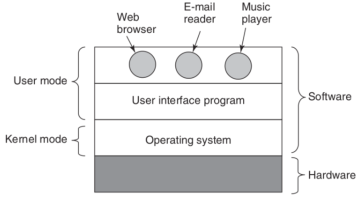
\includegraphics[width=0.85\textwidth]{FIG/1-1.pdf}
		\caption{操作系统所在的位置}\label{fig:fitin}
	\end{figure}

	同时,在许多系统中,一些用户态的程序协助操作系统完成特权功能。例如,经常有一些程序允许用户们修改密码,但是这个程序不是操作系统的一部分也不运行在内核态,但是它执行明显的敏感功能,并且必须以某种方式给予保护。
	在一些系统中,这个想法被执行到了极致,一些传统的被认为是操作系统一部分的程序运行在了用户态。在这些系统中,很难去划分一个界限,运行在内核态的明显是操作系统的一部分,然而运行在内核态之外的程序也有争议地被认为是操作系统的一部分,或者至少与其紧密相关。
	
	操作系统与应用程序的差异不仅仅在于他们所处的位置,特别地,操作系统更加大型,复杂和长期存在。像Linux和Windows这样的操作系统的核心代码都在500万行以上,要理解这个数量的含义,设想一下将500万行代码打印出来,每页50行,每卷1000页,将会需要100卷来打印出整个操作系统,需要一整个书柜来存放。你可以想象一下你获得了一个维护操作系统的工作,第一天你的老板把你带到存放代码的书柜面前,告诉你:学习这些代码吧。而这仅仅是运行在内核态的代码,当必要的共享库被包括进来的时候,Windows将会有将近7000万行代码,可以装满10-20个书柜。而这还不包括基础的应用程序(如窗口浏览器和媒体播放器等)。
	
	至于为什么操作系统的寿命较长,是因为它是非常难写的,一旦写了一个,所有者当然不愿意把它扔掉再重写一个。相反,操作系统会在长时间内进行演化。Windows 95/98/ME基本上是一个操作系统,Windows NT/2000/XP/Vista/Windows 7基本上是另一个操作系统。他们对于用户非常地相似,因为微软在努力使得Windows NT/2000/XP/Vista/Windows 7系统和Windows 98的系统非常相似。无论如何,微软要舍弃Windows 98是有非常好的理由的,我们将在第十一章中详细解释。除了Windows,我们在本书中用到的主要例子是UNIX以及它的变种和克隆版。UNIX当然也演化了很多年,如System V,Solaris和FreeBSD都是从该版本中演化出来的,尽管Linux像依照UNIX模式仿制而成,并且与UNIX高度兼容,但是其具有全新的代码基础。本书将采用来自UNIX的示例,并且在第十章中详细讨论Linux。
	
	在本章中,我们将简要触及操作系统的几个关键方面,包括它们是什么,它们的历史,有哪些分类,一些基本概念和它们的结构等。在后续的章节中,我们将详细介绍这些重要的内容。

\section{什么是操作系统}

	很难去给操作系统下一个明确的定义,操作系统是一个运行在内核态的软件,尽管这种说法并不完全符合事实。部分原因是操作系统扮演着两个完全不相关的功能,提供非应用程序编程人员一个清晰的资源集抽象而不是一堆混乱的硬件,并同时管理好这些硬件资源。取决于谁在谈论这个问题,你可能只会听到其中一个功能或另一个功能,让我们同时谈论这两个功能。
	
\subsection{操作系统作为一台扩展的机器}

	大多数计算机在机器语言级别的架构(指令级、内存组织、IO和总线结构)是原始的和难以编程的,特别是输入/输出。为了更细致地考察这一点,我们以在大多数计算机上使用的现代SATA硬盘位为例,曾有一本书描述早期版本的硬盘接口,一个程序员为了使用硬盘而应该了解的东西,超过了450页。自比2007年起,这个接口被修改了很多次,并且比那时候复杂了许多。很明显,没有任何一个理智的程序员想要在硬件层面和硬盘打交道,相反,他们使用一个叫做磁盘驱动的软件和硬盘打交道,这类软件提供了读写硬盘的接口,而不用去深入细节。操作系统包含了许多类似的控制IO设备的接口和驱动程序。但是即使是在这个层面,对于大多数应用程序而言还是太底层了。因为这个原因,所有的操作系统还提供另外一层使用磁盘的抽象:文件。使用这个抽象,程序可以创建、写和读文件,而不用去和底层硬件实际是如何工作的繁琐细节打交道了。
	抽象是管理这种复杂性的一种关键。良好的抽象可以将一个近乎不可能完成的任务转换为两个可以掌控的任务。第一步是定义和实现这些抽象,第二部是使用这些抽象来解决手头上的问题。一个几乎所有的计算机使用者都理解的抽象是文件,正如上文所提到的。它是一个有用的信息片段,像数字图片,保存的邮件消息,歌曲或者网页等。处理图片,邮件,歌曲和网页比处理SATA接口硬盘的细节要容易得多。操作系统的工作就是创建良好的抽象,并实现和管理它所创建的抽象对象。在本书中,我们将会讨论到许多关于抽象的内容,因为这是理解操作系统的关键。
	
	这点是如此地重要以至于它值得用不同的词语来重复描述。尽管出于对设计Macintosh机器的工程师的尊重,我们还是不得不说,硬件是丑陋的。真实的处理器、内存、磁盘和其他的设备是非常复杂的,对于那些必须使用它们来编写软件的人们而言,呈现出来的接口是困难、可怕、怪异和不一致的接口。有些时候这个是为了向后兼容更老一些的硬件,有的时候是为了节省成本。通常,硬件设计师们并没有意识到他们给软件的设计者们带来了多大的麻烦。操作系统的一个主要任务是隐藏硬件的细节,呈现给程序(和编程者)一个良好、清晰、简洁和一致的抽象。操作系统将丑陋转化为美丽,如图 \ref{fig:uglybeautiful} 所示。
	

	\begin{figure}[ht]\small
		\centering
		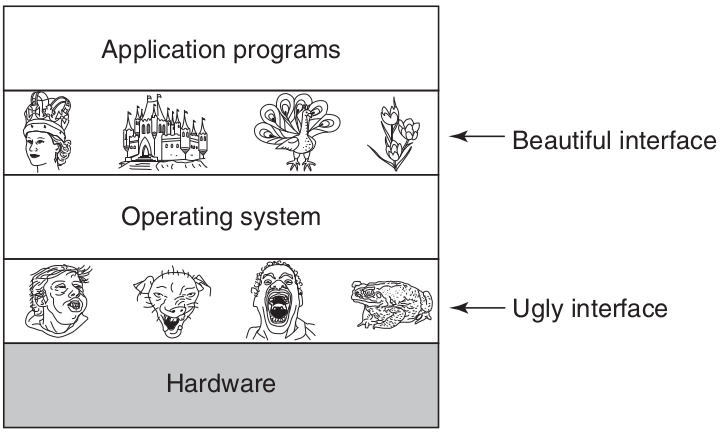
\includegraphics[width=0.75\textwidth]{FIG/1-2.png}
		\caption{操作系统将丑陋的硬件转化为美丽的抽象}\label{fig:uglybeautiful}
	\end{figure}

	值得注意的是,操作系统真正的消费者是应用程序(当然,通过应用程序的编程者),他们直接和操作系统及其抽象打交道。相比较而言,终端用户与应用接口所提供的抽象打交道,或者是命令行shell或者是图形用户界面。而用户接口的抽象可以和操作系统提供的抽象类似,但也不总是这样。为了更清晰地说明这一点,请读者考虑通常的Windows桌面和面向行的命令提示符。两者都运行在Windows操作系统上并且使用Windows提供的抽象,但是他们提供的是非常不同的用户接口。类似地,一个运行Gnome和KDE的Linux的用户和一个直接工作在X Window系统上的Linux用户看到的也是非常不一样的接口,但是两者的底层操作系统抽象是一致的。在本书中,我们将在细节层面讨论提供给应用程序的抽象,但是对于用户接口将讨论不多。尽管用户界面是一个重大且重要的主题,但是它只是与操作系统的外围相关。

\subsection{作为资源管理者的操作系统}

	把操作系统视为向应用程序提供抽象的概念是一种自顶向下的视角。按照另一种自底向上的视角,操作系统是用来管理一个复杂系统的各个部分。现代计算机包括处理器、内存、定时器、磁盘、鼠标、网络接口、打印机以及许多其他设备。在自底向上的视角,操作系统的工作是提供对需要处理器、内存和I/O设备等硬件资源的应用程序提供有序和可控的分配。现代操作系统允许在内存中同时运行多道程序,想象一下如果运行在同一台计算机上的三个程序同时想向打印机打印出它们的输出。第一个回合,我们将研究连续几代的计算机,看看它们的操作系统是什么样的,这种将操作系统的代际映射为计算机代际的做法是粗糙的,但是它确实提供了一种结构,否则就没有这种结构。接下来给出的进程主要是以时间顺序展开的,但是它又是一个颠簸的旅程。每一个发展阶段都不是等着上一个发展阶段完美地结束后才开始的,阶段与阶段之间有很多的交集,更不用说很多错误的开始和死胡同,请把这个作为一个向导,而不是一个定论。
	第一台真正的数字计算机是由英国数学家查尔斯·巴贝奇(1792–1871)设计的,尽管巴贝奇花费了他一生中大多数的时间与财富试图构建他的“分析机”,可是他从没有能够让它正常地工作,因为这个机器是纯机械式的,在当时他所在的年代,还不能制造出能够满足他所需的高精度的轮子、齿轮和轮齿。无需赘言,他的“分析机”也没有一个操作系统。
	作为一个有趣的历史旁白,巴贝奇意识到他的“分析机”可能需要软件,所以他就雇佣了一个叫阿达·洛芙莱斯的年轻女性作为程序员,她就是英国著名诗人拜伦勋爵的女儿,是世界上第一位程序员,编程语言Ada就是以她的名字命名的。
	
\section{操作系统历史}

\subsection{第一代(1945-55)真空管}

	在巴贝奇不成功的努力后,电子计算机的发展直到第二次世界大战之前取得了进步都很小,刺激了活动的爆发。John Atanasoff教授和他的研究生Clifford Berry在爱荷华州立大学建造了第一个功能式的电子计算机,它用了300个真空管。几乎与此同时,柏林的Konrad Zuse用机电继电器制造了Z3计算机。在1944年,一群科学家(包括阿兰图灵)在英格兰的伯克利公园制造和编写了Colossus机器,Howard Aiken在哈佛大学制造了Mark I,William Mauchley和他的研究生J. Presper Eckert在宾夕法尼亚大学制造了ENIAC。这些机器,一些用二极管,一些用真空管,一些是可编程的,但是都非常地原始,即使是进行最简单的计算也要耗用数秒钟的时间。
	在早年,同一小组的人们(通常是工程师们),设计、建造、编程、操作和维护每一台机器。所有的编程都是用绝对的机器语言完成的,更为糟糕的是,需要通过将上千根电缆插到插线板上连接成电路,以便控制机器的基本功能。没有程序设计语言(甚至连汇编语言也没有),操作系统更是从来就没有听说过。那时程序员一般的操作方式是,在墙上的机时表上预约一段时间,然后到机房中将他的插线板接到计算机里,接下来就是在接下来的几个小时里期盼计算机里的两万多个真空管不会被烧坏。那时,所有的问题都只是简单的数学和算术运算,如制作正弦、余弦、对数表或者是计算弹道轨迹等。
	在20世纪50年代,情形有了一定的改善,出现了穿孔卡片,这样就可以将程序写在卡片上,读入计算机而不再使用电路板,然后,其他的过程还是一样的。
	
\subsection{第二代(1955-65)晶体管和批处理系统}

	在上世纪50年代出现的晶体管的发明,极大地改变了这个状况。计算机已经变得很可靠,它们可以被制造、生产和出售给消费者,并且它们可以工作足够长的时间来完成一些有用的工作。就这样,第一次在设计者、制造者、操作者、编程者和维护者之间有了一个明确的分工。
	这些机器,现在叫做大型机,被锁在有专用空调的大机房里,有工作人员和专业操作者来运行他们。只有一些大型的公司,主要的政府机构和大学可以负担数百万美元的价格。为了运行一个任务,程序员需要首先将程序写在纸上(使用FORTRAN或者汇编语言),并把它做成有孔卡片,再将卡片盒带到输入室并把他交给操作人员,接下来就是边喝咖啡边等待输出结果的完成。
	
	当计算机完成了正在进行的任何的工作,操作者都要到打印机前撕下运算结果并把它带到输出室,以便程序员稍后收集、整理。然后,操作员将另一个卡片盒带到输入室并读入另一个任务。如果需要FORTAN的编译器,操作者需要将它从文件柜中取出并读入输入室中。大部分的机器时间在操作员在机器室中走来走去的时候被浪费掉了。

	因为设备具有这么高的成本,因此人们迅速地开始寻找降低所浪费时间的方法也就可以理解了。通常采用的解决方法是批处理系统(Batch System)。
	它背后的想法是将一堆工作收集起来放到输入室中,并用一个不太昂贵的机器例如IBM 1401将它读入磁带中,该机器非常擅长读取卡片,复制磁盘,打印输出结果,但是并不擅长数值计算。而真正擅长数值计算的机器,如IBM 7094,用来执行实际的运算。其情形如图 \ref{fig:batchsystem} 所示。
	
	\begin{figure}[ht]\small
		\centering
		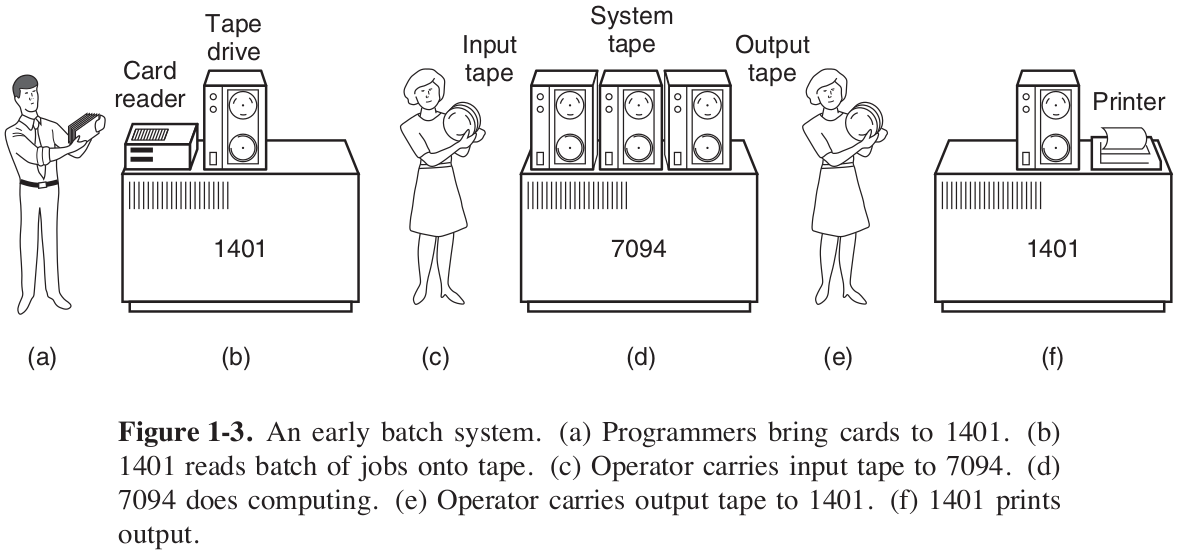
\includegraphics[width=0.75\textwidth]{FIG/1-3.png}
		\caption{一个早期的批处理系统}\label{fig:batchsystem}
	\end{figure}

	当一个完整的批处理过程结束的时候,操作员移除输入和输出的磁带,替换成下一批的输入磁带,并把上一批的输出磁带在一台1401的机器上离线打印出来(而不是连接主计算机)。
	
	一个典型的输入任务的结构如图 \ref{fig:FMS} 所示。它开始于一个\$JOB卡片,以分钟为单位设置好最大的运行时间,计费帐号以及程序员的名字。接着是一个\$FORTRAN卡片,告诉操作系统从系统磁带上加载FORTRAN的编译器,之后就是待编译的源程序,接着是一个\$LOAD卡片,直接地操作系统加载刚刚编译的目标程序。(编译程序通常被写在刮插磁带上并且需要被显式地加载)接下来是\$RUN卡片,告诉操作系统运行程序并使用随后的数据。最后,\$END卡片标志工作的结束。这个原始的控制卡片是现代shell和命令行解释器的先驱。
	
	\begin{figure}[ht]\small
		\centering
		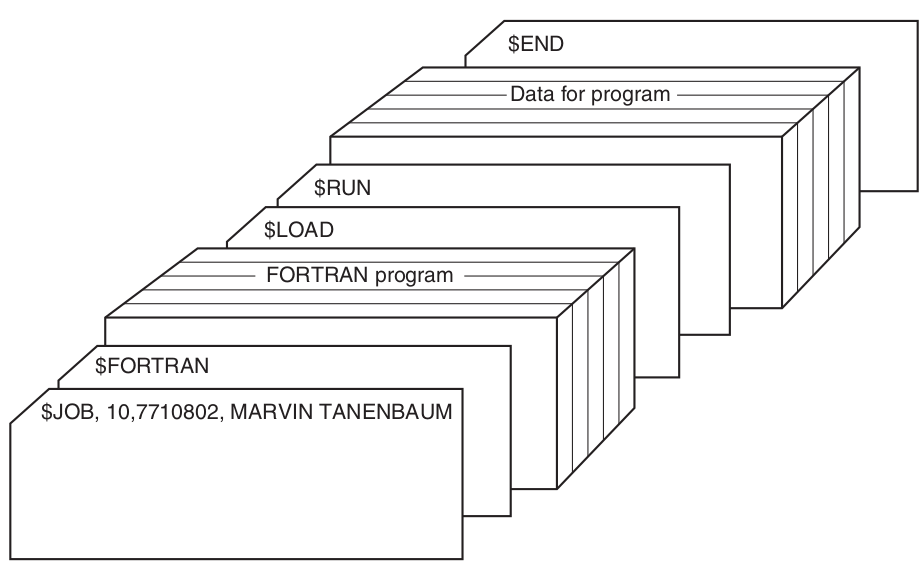
\includegraphics[width=0.75\textwidth]{FIG/1-4.png}
		\caption{一个典型的FMS作业结构}\label{fig:FMS}
	\end{figure}

	第二代大型计算机主要用于科学与工程计算,像在物理和工程中经常出现的解偏微分方程的程序,他们通常是使用FORTRAN和汇编语言编写的。典型的操作系统是FMS(Fortran Monitor System)和IBSYS,IBM的操作系统是7094。
	
\subsection{第三代(1965-1980)集成电路和多道程序设计}

	在上世纪60年代,大多数计算机生成厂商都有两条完全不同的,互不兼容的生产线。一种是是面向文字的,大规模的科学计算机,像7094,常用来在科学和工程领域进行工业级的数值计算。另一种是,面向字符的商用计算机,像1401机器,被银行和保险公司广泛地运用于磁带排序和打印上。
	
	发展和维护两个完全不一样的生产线对于生产厂商而言是一项昂贵的任务。此外,许多新的计算机消费者一开始仅仅需要一个小的机器,但是随着业务量的增长,他们需要一个更大的机器来运行他们的旧程序,但是需要运行地更快一些。
	
	IBM试图通过System/360系统来一举同时解决以上两个问题。360是一系列软件兼容的机器,从与1401机器相当的低端机器到与7094机器相当的高端机器。这些机器只是在性能和价格上(最大内存、处理器速度、允许接入的I/O设备的数量)的差别。因为他们拥有相同的架构和指令集,在一台机器上编写的程序可以在其他的任何机器上运行,至少理论上是。(但是,正像Yogi Berra说的这样,在理论上,理论和实际是一致的,但是在实际上,它们却不是。)因为360机器是被设计用来处理科学和商业计算,那么一个单系列的计算机可以满足所有客户的需求。在随后的几年里,IBM使用现代技术出产了360机器的后续机型,像370,4300,3080和3090。zSeries是这个系列的最新机型,不过它与早期的机型相比变化非常之大。
	
	IBM360机器是第一代采用小规模集成电路的主流机型,因此比采用分立晶体管的第二代的机器具有很高的性价比。360机器很快获得了成功,而且系列兼容机的想法很快被其他计算机制造厂商接受了。这些计算机的后代仍然在大型计算中心中使用,现在他们经常被用来维护大型的数据库系统(例如,航空订票系统)或者作为Web站点的服务器,这些服务器必须每秒处理上千次的请求。
	
	“单系列”想法的最大优点同时也是它的最大弱点。最初的意图是,所有的软件,包括操作系统OS/360原本都打算在所有的机器上运行。从小的能够替代1401机将卡片转换为磁带,到大的机器能够代替7094机器进行天气预报和其他繁重计算任务的计算任务。从只能带很少外部设备的机器到有很多外设的机器,从商业领域到科学领域。总之,它必须适用于所有的这些不同的用途。
	
	IBM无法写出能够同时满足这些相互矛盾的需求的软件,其结果是一个庞大而又复杂的操作系统,大概比FMS系统复杂2-3个数量级。它包括数千名程序员写的数百万行的汇编代码,同时包含数千个bug,这也导致IBM不断地发布新的版本来修正这些错误。每个新版本在修复就的bug的同时也引入了新的bug,因此bug的数量可能随和时间的变化而基本保持不变。
	
	作为OS/360的设计者之一的Fred Brooks,后来写了一本诙谐又尖锐的书籍来描述他对OS/360系统的经验。在这里不可能总结书中的内容,不过它的封面已经充分表达了它的观点,一群史前巨兽陷入了泥潭中不能自拔。Silberschatz书的封面也表达了类似的观点,操作系统像是恐龙一样。
	
	尽管OS/360有着巨大的规模和问题,OS/360和其他厂商开发的第三代操作系统实际满足了消费者大部分的需求。他们同时还使第二代操作系统中缺乏的几项关键技术得到了广泛的应用。其中一个重要的技术是多道程序设计(multi programming)。在7904机上,当当前的工作任务需要暂停来等待一个磁带或者I/O操作结束的时候,CPU仅仅是空闲等待I/O操作的完成。在CPU密集型的科学计算任务中,I/O操作是不频繁的,所以浪费的时间不是很明显。在商业数据处理的工作任务中,I/O等待的时间可能占用全部时间的80\%到90\%,所以必须采取某些措施来避免昂贵的CPU空闲这么久。
	
	所采用的方式是将内存分为几个分区,每一个分区中存放一个不同的作业,如图 所示。当一个作业在等待IO操作完成的时候,另一个作业可以继续使用CPU。如果有足够多的工作任务驻留在内存中,CPU可以保持接近100\%的使用时间。同时在内存中安全地保存数个工作任务,需要专门的硬件来保护每个工作被其他的工作所窥测和损害,360机器和其他的第三代系统都配备了这个意见。
	
	\begin{figure}[ht]\small
		\centering
		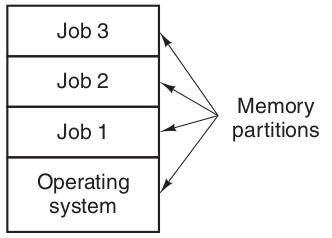
\includegraphics[width=0.65\textwidth]{FIG/1-5.png}
		\caption{一个有三个程序在内存中的多道程序系统}\label{fig:multiprogramming}
	\end{figure}

	第三代操作系统另一个主要的特征是具备了尽快将带到机房的磁带上的作业内容读取到磁盘上。因此,当一个运行中的作业停止的时候,操作系统可以从磁盘中加载一个新的作业到非空的内存区域中并运行它。这个技术叫做SPOOLing(外部设备联机并行操作),该技术也同时用于输出。因为有了SPOOLing技术,1401机器就不再需要了,而且也不需要将磁带搬来搬去了。
	
	尽管第三代操作系统非常适用于大型的科学计算和大部分商业数据的处理,它们基本还是批处理系统。许多编程者很怀念第一代机器的编程模式,那时他们可以单独占用机器好几个小时,从而可以调试自己的程序。在第三代操作系统中,从一个作业任务提交到获取输出结果通常需要好几个小时,因此一个分号的误用都有可能导致编译的失败,而可能浪费了程序员大半天的时间,程序员是非常不喜欢这种情况的。
	
	对快速响应时间的渴望对分时复用铺平了道路,一个多道程序的变化版,每一个用户都有一个联机终端。在一个分时系统中,如果有20个用户登录了系统,而其中有17个用户在思考,在交谈或者在喝咖啡,则CPU可以分配给三个需要服务的作业。因为人们在调试程序的时候经常使用较短的命令(编译一个5页的源文件)而不是较长的命令(对一个有100万件记录的文件进行排序)。计算机可以为一些用户提供快速的,交互的服务,或者在CPU空闲的时在后台同时处理的大型的批处理作业。第一代通用的分时操作系统CTSS,是在MIT基于一台修改的7904机器实现的。然而,分时复用系统没有得到及时的使用直到必要的保护硬件在第三代操作系统中出现。
	
	在CTSS系统成功之后,M.I.T.,贝尔实验室和通用电气(那时还是一个主要的计算机制造商),决定着手开发“计算机实用程序”,支持数百个同时分时用户的机器。他们的模型是电能系统,当你需要电能的时候,你只需要把用电设备插入墙上的插座即可,于是,在合理范围之内,所需要的电能随时可以提供。这个系统的设计者,被称作“MULTICS”系统,着眼于使用一个巨型的机器来为波士顿地区的每一个人提供计算能力。在当时看来,仅仅40年以后,就可以成百万台地卖掉比GE-645机器快1万倍的机器(价格远远低于1000美金),是纯粹的科幻,类似于现在的跨大西洋超音速海底列车的想法。
	
	MULTICS是一个混合的成功。它仅仅被设计在仅仅比基于Intel 386的PC机器强一点的机器上同时支持上百个用户,尽管它具有更高的I/O容量。可是这个想法并不用表面看上去这么荒唐,因为那个时候人们知道如何写小的、有效的程序,这个技能在后来逐渐消失了。MULTICS没有能普及到全世界是有很多原因的,其中一个重要的原因是它是用PL/I编程语言编写的,PL/I编译器的开发延迟了好几年,好不容易完成的编译器又很少能够正常地运行。当时,MULTICS有着很大的野心,就像19世纪查理斯巴贝奇的分析机器一样。
	
	简要地说,MULTICS向计算机文化中传播了许多原创的观念,但是要把它打造成一个严谨的产品和一个主要的商业成功则不那么容易。贝尔实验室放弃了这个计划,而通用电气也一起退出了个人电脑的业务。但是,MIT坚持了下来并让MULTICS最终得到运行。它最终被作为一个商业产品被收购了GE公司计算机业务的Honeywell公司出售,并且被超过80家的公司和大学安装使用了。尽管用户不多,但是MULTICS的用户是极度忠诚的。
	在试图让Honeywell公司更新硬件多年以后,通用汽车,福特,美国国家安全局在上世纪90年代末期才停止运行MULTICS,而这时距离MULTICS的发布已经过去了30多年。
	
	到20世纪末期,服务计算的概念已经被遗弃了,但是现在又以云计算的形式回归了,相对小的机器(包括智能手机、平板电脑)连接到遥远而又巨大的数据中心服务器在那里所有的计算都被完成,而本地计算机仅仅只是处理用户接口程序。这里的动机是多数人不愿意管理日益复杂的计算机系统,而更倾向于让运营、维护数据中心的专业团队去做这些事情。电子商务已经朝这个方向发展,许多公司都在多处理器服务器上运行邮件服务,简单的客户机连接到多处理器的服务器上,非常符合MULTICS的设计思想。
	
	尽管MULTICS没能取得商业上的成功,MULTICS对接下来的操作系统产生了及其重要的影响(特别是UNIX和它的衍生系统,如FreeBSD、Linux、iOS和Android系统)。详情请参考相关文献和书籍。还有一个活跃的网站,网址是www.multicians.org,上面有大量的关于该系统、设计者和用户的信息。
	
	第三代操作系统另一个重大的发展是小型计算机的崛起与快速发展,以1961年DEC的PDP-1机器为起点。PDP-1计算机只有4K个18位的内存,但是每台机器的售价是12万美元(仍不到7094机器的5\%),该机型非常地热销。对于一些特定的非数值型的计算任务,它和7904机器几乎一样快,并且催生了一个产业,并且很快有了其他一系列PDP机型(不像IBM家族,他们都是非兼容的),其顶峰为PDP-11。
	
	贝尔实验室的计算机科学家肯托马森,找到了一个无人在用的PDP-7小型计算机,开发了一个简化的、单用户版本的MULTICS,这个系统后来就发展成了UNIX系统,并且在学术界、政府机关和许多公司得到了广泛的使用。UNIX的历史已经在别处被多次讲述了,这段故事的一部分将在第10章中进行讲述。现在,因为源代码可以到处被得到,不同的组织会发展他们不同的版本,因而导致混乱。两个主要的版本被开发出来了,一个是AT\&T的System V系统,另一个是加州伯克利分校的FreeBSD系统,当然还有一些其他的小的变种。为了能够使编写的程序运行在任意的UNIX系统上,IEEE为UNIX开发了一套标准,该标准被称为POSIX标准,是现有大多数的UNIX支持的版本。POSIX定义了符合UNIX系统必须支持的最小系统调用接口。事实上,其他一些操作系统现在也支持POSIX接口。
	
	值得一提的是,在1987年,本书作者发布了一款UNIX的克隆版本,称为MINIX,用作教育目的。在功能上,MINIX非常类似与UNIX,包括POSIX的接口支持。从那以后,原来的版本已经演化为MINIX3了,它高度模块化,并且专注于非常高的可用性。它具有在不重启和不打扰其他运行程序的情况下,运行时检测和替换错误甚至是崩溃模块的能力,它致力于提高可用性和可靠性。有一本列出内部操作和在附录中列出源代码的书籍现在还有出售。MINIX 3系统是完全免费的,源代码可以在www.minix3.org上获得。
	
	对与MINIX系统自由产品的渴望,促使一位芬兰学生Linus Torvalds来撰写Linux。这个系统被直接受MINIX系统的启发,并且一开始就支持不同的MINIX的特征(例如,MINIX文件系统)。它被许多人在许多地方做了扩展,并且保持了许多与MINIX和UNIX类似的底层结构。对Linux的详细历史和开源运动感兴趣的读者们可能想读Glyn Moody的书,
	%在书中反复提到的是UNIX被应用到System V,MINIX,Linux和其他UNIX系统的克隆版本中去
	本书所包含的许多内容也同样适用于System V,MINIX,Linux以及UNIX的其他版本与克隆。

\subsection{第四代(1980-现在)个人计算机}

	随着大规模集成电路(LSI)的发展,在一平方厘米的硅片芯片上包含上千个晶体管,个人计算机的时代来临了。在架构方面,个人计算机(一开始称为微机)和PDP-11系列的小型计算机相比并没有很大的不同,但是在价格上却差别了很多。小型计算机的出现使得一个大学或公司的部分可以拥有自己的计算机,微处理器芯片的诞生则使得个人拥有自己的计算机称为了可能。
	1974年,Intel推出了8080CPU,第一款8位的通用CPU。它需要一个为8080设计的操作系统,一部分目的是为了对其进行测试。于是,Intel就安排了其顾问Gary Kildall来为8080CPU写操作系统。
	Kildall和他的朋友首先为新发型的Shugart Associates8英寸磁盘设计了一个控制器,并将软件连接到8080CPU,从而生产出第一台带有软盘的微型计算机。Kildall进而编写了一款基于磁盘的操作系统(CP/M (Control Program for Microcomputers))。因为Intel认为基于磁盘的个人计算机可能前途不大,当Kildall要求拥有对CP/M的所有权的时候,Intel答应了他的要求。Kildall进而创建了一个公司,Digital Research,来继续发展和销售CP/M。
	1977年,Digital Research公司重写了CP/M操作系统,使得它可以更好地运行在使用8080,Zilog Z80和其他CPU芯片的微型计算机上。并且基于CP/M编写了许多应用程序,使得CP/M系统主宰了微型计算机领域长达5年的时间。
	在20世纪80年代早期,IBM设计了IBM的PC并且寻找运行在其上面的软件。来自IBM的员工联系了Bill Gates来获得他的BASIC解释器的版权。他们还问他是否有运行在PC上的操作系统,Gates建议他们联系Digital Research公司,当时世界上操作系统的主流公司。作为有史以来最糟糕的商业决定,Kildall拒绝了和IBM的会面,而是让一名下属接待了他。更糟糕的是,他的律师甚至拒绝签署IBM关于对尚未公开的PC的保密协议。接下来,IBM公司只好回来找Gates,问他是否可以提供他们一个操作系统。
	
	当IBM回去的时候,Bill Gates想到一家当地计算机制造商,西雅图计算机产品公司,有一款合适的计算机系统,DOS(磁盘操作系统)。他与他们接洽并提出要购买这个操作系统,据说价格为75000美元,他们立即答应了。于是Gates提供给IBM一个DOS/BASIC的包,IBM接受了。IBM想要进行一些修改,所以Gate雇佣了写作DOS的人蒂姆·帕特森作为Gates的新公司微软的雇员也进行这项工作。被修改的系统被改称为微软DOS系统,并且很快地开始主导IBM的PC机市场。与Kildall试图将CP/M每次卖给一个用户相比(至少一开始是这样)相比,在这里一个关键的因素,后来也被证明是非常明智的决定的是Gates决定将他们的MS-DOS操作系统和计算机公司的的硬件绑定起来一起销售。在这所有的一切烟消云散之后,Kildall突然离开了人世,其原因至今仍没有被完全披露。
	
	IBM PC的继任者IBM PC/AT,在1983年随着Intel 80286CPU一起被开发出来。至此,MS-DOS的地位开始牢固确立,而CP/M只剩下了最后的支撑。MS-DOS后来被广泛使用于80386和80486CPU之上。
	尽管MS-DOS的初始版本非常地原始,后续的版本包含了很多高级的特征,包括许多从UNIX借鉴的特征。(微软对于UNIX是如此地娴熟,以至于在公司的早期还销售过一款叫做XENIX的微型计算机版本)
	
	早期的微型计算机的操作系统,CP/M,MS-DOS和其他的操作系统都是基于用户从键盘输入命令的方式。这种情况被斯坦福研究所的Doug Engelbart在上世纪60年代的研究所最终改变了。道格·恩格尔巴特发明了图形用户界面,有完整的窗口,图标,菜单和鼠标。这些想法被施乐PARC的研究人员采纳,并被融入到他们制造的机器中。
	
	一天,当史蒂夫乔布斯在他的车库中联合创建了苹果电脑公司,访问了PARC,看到了GUI,立即意识到了他的潜在价值,而Xerox管理层恰好没有意识到。这种战略失误的庞大比例,导致了名为《摸索未来》一书的出版。
	乔布斯随后着手设计了带有GUI的苹果计算机,这个工程导致了Lisa的诞生,但是由于价格过于昂贵导致了商业上的失败。乔布斯的第二次尝试,苹果的Macintosh电脑,取得了巨大的成功,不仅是因为它比Lisa便宜很多,而且还因为它是用户友好的。这就意味着它的用户不仅可以对计算机一无所知,而且可以完全没有任何学习的意图。在图片设计,专业数字图片和专业数字视频生产领域,Macintosh获得了广泛的应用,并且这些用户对Macintosh有着极大的热情。1999年,苹果公司采用了一种内核,它来自本是为替换BSD UNIX内核而开发的卡内基梅隆大学的Mach微核。因此,尽管有着完全不同的界面,但是Mac OS X是基于UNIX的操作系统。
	
	当微软决定构建MS-DOS的后继产品时,它受到了Macintosh电脑成功的强烈影响。它构建了一个基于GUI的桌面操作系统,最初是运行在MS-DOS之上的(它更像是一个shell界面而不是一个操作系统)。在接下来将近10年的时间里,从1985年到1995年,Windows都只是基于MS-DOS的一个桌面环境。然后,到了1995年,一个整合了许多操作系统特征的独立的Windows版本Windows95发布了。该系统仅仅将底层的MS-DOS系统用于启动和运行一些老的基于MS-DOS的程序。1998年,这个操作系统的一个稍作修改的版本Windows98发布了。但是,不管是Windows95还是Windows98,还都使用了大量的16位的Intel汇编语言。
	
	另一个Windows的操作系统,Windows NT(NT意味着New Technology),在一定程度上兼容Windows 95,但是其内部是完全重写的,它是一个完全的32位系统。Windows NT的主要设计者是David Cutler,他同时也是VAX/VMS系统的设计者,因此一些来自于VMS的系统也反映在了Window NT中。事实上,如此多的VMS的想法出现在Windows NT中,以至于VMS的所有者DEC公司,起诉了微软公司。法院对该案件的判决结果引出了一大笔需要用多位数字表达的金钱。微软公司期待NT的第一个版本将会打败MS-DOS和其他所有的Windows版本,因为Windows NT是一个巨大的超级系统,但是这个想法失败了。只有Windows NT 4.0踏上了成功之路,特别是在合作网络上。Windows NT 5.0在1999年初改名为Windows 2000。微软期待它成为Windows 98和Windows NT的替代者。
	
	不过这两个版本都不是很成功,微软稍后发布了Windows 98的另外一个版本Windows ME(千年版)。2001年,又发布了Window 2000的一个微升级版,我们称为Windows XP。这个版本运行的时间较长,并且替代了Windows的所有原始版本。
	
	版本的更替还在继续,在Windows 2000之后,微软将Windows家族分割成客户端和服务器端两条线。客户端基于XP和它的继承者,服务器端则包括Windows Server 2003和2008。第三条线,嵌入式系统也在随后出现。Windows的所有版本均已服务包的形式派生出各自的变种,这足以让系统的管理员以及操作系统书籍的作者感到温暖。
	
	2007年1月,微软终于发布了Windows XP的继承者,称为Vista。它有一个全新的界面,改善了安全性和许多新的和升级的用户程序。微软期望它可以完全地取代Windows XP,但是它并没有做到。相反,由于它对系统配置的较高要求,严格的版权条件和支持数据版权管理功能(一种使用户更难复制所保护资料的技术),使得它获得了大量的批评,负面报道不断。
	
	随着一款全新的且并不那么消耗资源的操作系统Windows 7的来临,许多人决定跳过Vista。Window 7并没有引入很多的新功能,但是它相对较小而且更为稳定。在不到3周的时间里,Windows 7就获得了比Vista在
	7个月内获得的更多的市场份额。2012年,Windows发布了Windows 7的继任者,Windows 8,一款针对触摸屏幕,拥有全新界面和感官的操作系统。微软希望这个操作系统会成为许多设备的主流操作系统:台式机,便携式电脑,笔记本电脑,手机,家庭影院电脑等主流的操作系统。然而,到目前为止,它的市场占有率的渗透远远慢于Windows 7。
	
	另一个在个人电脑操作系统市场上的有力竞争者是UNIX(以及它的不同变种)。UNIX在网络和企业服务器上很强,但是也经常出现在台式电脑,笔记本电脑,平板电脑和智能手机上。在基于X86架构的计算机上,Linux正在成为学生和越来越多的企业用户代替Windows的受欢迎的替代者。从一个侧面,贯穿本书我们都将使用术语X86来指代从1970年代开始8086相同指令集架构的现代处理器。
	
	有许多的AMD或者Intel公司生产的处理器,	在引擎盖下它们或许有一些不同,处理器是32位的或者64位的,单核或者多核的,流水线深的或者浅的,不一而足。不管怎么样的,对于编程者而言,它们看起来都是相似的,并且都可以运行35年前的代码。尽管这种不管是很重要的,我们将使用显式模型,并且使用X86-32或者X86-64来指示32位或者64位的变体。
	
	FreeBSD同样也是UNIX的一个流行变体,它来源于伯克利的BSD项目。所有的现代Macintosh的计算机都运行的是FreeBSD的修改版本(OS X)。在使用高性能RISC芯片的工作站上,UNIX也是一个标准配置。
	它的变体广泛应用于移动设备中,像运行iOS 7和Android的设备。许多UNIX用户,特别是有经验的编程人员,比起GUI更加喜欢使用命令行界面。所以,所有的UNIX系统支持一个在MIT生产的叫做X Windows的系统(也被称为X11系统)。这个系统处理基本的桌面管理,允许用户使用鼠标创建、删除、移动和改变窗口的大小。经常一个完整的GUI,像GNOM或者KDE,可以运行在X11之上,使得UNIX给人一种类似于Macintosh或者微软Windows系统的感觉,对于那些想要这样做的UNIX用户而言。
	
	开始发生在上世纪80年代中期的一个有趣的发展是,运行网络操作系统和分布式操作系统的个人计算机网络的增长。在一个网络操作系统中,用户可以感知到多台计算机的存在,并且允许从一台机器向另一台机器复制文件。每一台机器都运行自己的本地文件系统并且有自己的本地用户。
	
	网络操作系统和单处理器的操作系统有着基本的不同。它们显示的需要一个网络接口控制器和一些低级别的软件来运行它,同时,程序获得远程登录和远程文件访问权限,但是这些附属并不改变操作系统的一个本质结构。
	
	一个分布式操作系统,相比较而言,它对用户呈现的还是一个传统的单处理器系统,即使是它实际上是包含多个处理器。用户可能不会感知到他的程序在哪里运行,他的文件存放在哪里,这些都是由操作系统来自动和有效地处理的。
	
	真正的分布式操作系统不仅仅是对单处理器操作系统增添一点代码那么简单,因为真正的分布式系统和集中式系统在一些关键方面有着很大的不同。分布式系统,例如,同时允许应用程序运行在好几个处理器上,因而为了优化并行量需要更多复杂的处理器调度算法。
	
	网络中的通信延迟意味着这些算法必须运行不完全的、过时的甚至是错误的信息。而这在一个单处理器系统中却有根本的不同,因为单处理器系统中操作系统掌握着整个系统状态的全部信息。
	
\subsection{第五代(1990-现在)移动计算机}

	自从迪克特雷西侦探在1940年代的连环画中开始使用“双向无线电腕表”,人们就渴望拥有一台可以随身携带的通讯设备。第一台真正的移动电话出现在1946年,重达40公斤。如果你有一辆汽车的话,你就可以把它带到任何地方。第一台真正的手持移动电话出现在1970年代,重量约1公斤,是绝对的羽量级,它被亲切地称为“砖头”,很快每个人都想拥有一台。今天,移动电话的使用率几乎覆盖了全世界90\%的人口。我们不仅可以使用移动电话和腕表打电话,并且很快可以使用眼镜和其他可穿戴设备打电话了。更多的是,打电话本身并不是很有趣了,我们可以收发邮件、网上冲浪、和朋友聊天、玩游戏和在交通拥堵中导航,甚至不需要想它两遍(一切都是那么地习以为常)。
	
	尽管将电话和计算功能集成到一个像电话一样的设备的想法在1970年代就出现了,第一台真正的智能电话直到1990年代NOKIA发布N9000才出现,它在表现上包含了两个完全独立的设备:移动电话和个人数据助手。在1997年,爱立信公司为它的GS88"Penelope"手机创建了“智能手机”一词。
	
	现在,智能手机已经无处不在了,不同的操作系统之间的竞争也非常地激烈,而且前景比PC世界还要晦暗不明。在编写此书的时候,谷歌的Android系统占有统治地位的操作系统,苹果的iOS系统则稳居次席。但是这种情形并不一定总是这样,并且有可能在几年内又会发生变化。如果在智能手机领域有什么是清楚的话,那就是长期占用山峰的王者地位是不容易的。
	
	大部分的智能手机在头十年中运行的操作系统是Symbian OS。它是一些流行厂商如三星、爱立信、摩托罗拉,特别是诺基亚选择的操作系统。然而,其他的操作系统像RIM的Blackberry OS(在2002年的智能手机中发布)和苹果的iOS(在2007年通过iPhone发布)开始蚕食Symbian OS的市场份额。许多人推测,RIM会占据主流市场,而iOS将会是消费者设备的王者,Symbian的市场份额暴跌。在2011年,诺基亚抛弃了Symbian并且声称将把Windows作为其主要的平台。在一段时间里,苹果和RIM被视为宠儿,尽管它们还没有达到Symbian曾经的流行程度和统治地位。但是这些并没有持续很长时间,谷歌在2008年发布的基于Linux的操作系统Android很快就战胜了它的对手。
	
	对于手机的生产商,Android的优势是它是开源的并且在一个开放的许可证下可以免费获得。因此,他们可以很容易地对系统做一些小的修补并适用于自己的硬件。同时,他还有一个庞大的开发APP的开发者社区,这些APP大部分是用Java语言写的。尽管如此,过去几年的形势表明Android的这种统治地位可能也持续不了,Android的竞争者们急于抢占它的一部分市场份额。我们将在第10.8节详细地介绍Android。
	
\section{计算机硬件概览}

	操作系统是和运行在其上的硬件设备紧密相关的,它扩展了计算机的指令集并管理它的资源。为了让其工作,你必须知道很多关于硬件的知识,至少要知道硬件是如何暴露给编程人员的。因为这个原因,让我们简要地回顾一下现代个人计算机中的硬件。完了以后,我们可以开始探讨操作系统的细节以及它是如何工作的。
	
	概念上讲,一个简单的个人计算机可以被抽象为如图 \ref{fig:components} 所示的类似模型。CPU、内存和I/O设备都通过一个系统总线连接,并通过它与其他部件通信。现代的个人计算机有一个更加复杂的结构,拥有多条总线,我们将在后面陆续讨论到。对于现在的时间点来说,现在的模型是足够了的。在接下来的章节中,我们将简要地介绍这些组件并且探讨一些关乎操作系统设计者的硬件的属性。毋须多言,将有一个非常紧凑的总结,许多书都是关于计算机硬件和计算机组织的,两本最著名的是Tanenbaum和Austin(2012)以及Patterson和Hennessy(2013)编写的两本。
	
	\begin{figure}[ht]\small
		\centering
		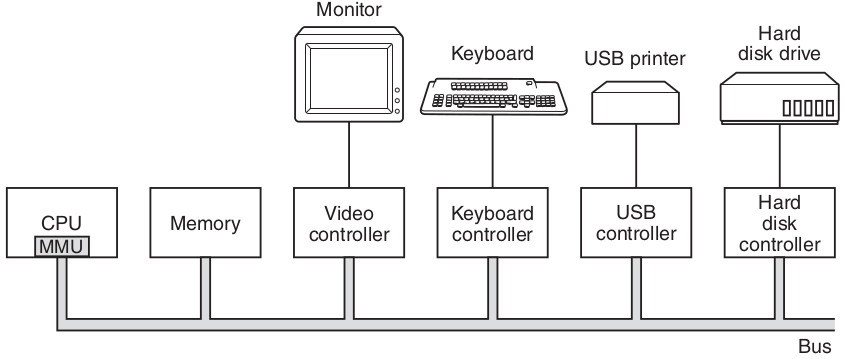
\includegraphics[width=0.65\textwidth]{FIG/1-6.png}
		\caption{一台个人计算机的主要组成部分}\label{fig:components}
	\end{figure}

\subsection{中央处理器}

	计算机的“大脑”是CPU。它从内存中获取指令并且执行它们。CPU的基本循环是从内存中获取第一个指令,解码这条指令来获取它的类型和操作数,执行它,接着再继续获取、解码和执行后续的指令,这个循环周而复始直到程序结束。通过这种方式,程序被执行。
	
	每一个CPU都有一个它可以执行的指令集,所以X86的处理器不能执行ARM的程序,ARM的处理器不能执行X86的程序。因为访问内存获取一条指令和数据比执行一条指令要花费很长的时间,所有的CPU都在内部保留一些寄存器来保存关键变量和中间结果。所以,指令集通常包含从内存中加载一个字段到寄存器的load指令,和将一个字段从寄存器存储到内存的store指令。其他的指令将来自寄存器、内存或者同时来自两者的两个操作数整合起来,像添加两个字段并且将结果存放在寄存器或者内存中。
	
	除了一些通用寄存器来存放变量和中间结果,大多数的计算机有几个对编程人员可见的专用寄存器,其中的一个是程序计数器,其中保存了下一条指令的内存地址。当那条指令被取出后,程序计数器的指针指向下一条指令。
	
	另外一个寄存器是栈指针,指向当前在内存中栈的顶部。栈包含每一个已经进入和尚未退出的程序中的一个页面,一个程序的栈页面保存这些没有存放到寄存器中的输入参数,局部变量和中间变量。
	
	另外一个寄存器是程序状态字(Program Status Word)。这个寄存器保存被比较指令设定的条件码位,CPU的优先权,模式(用户态或内核态),还有其他的各种控制位。用户程序可以读取程序状态字的所有位,但是只能写其中的某几个字段。PSW在系统调用和I/O中间发挥着重要的作用。
	
	操作系统必须对所有的寄存器实现完全的感知。当对CPU进行分时多路复用的时候,操作系统经常会停止目前正在运行的程序去启动或重启另一个程序。每次它运行一个程序,操作系统必须保存所有的寄存器状态,这样可以在后面重新启动被暂停的程序。
	
	为了改善性能,CPU的设计者们早就抛弃了同时取指、解码、执行一条指令的简单模型。许多现代的CPU具有同时执行一条或多条指令的功能。例如,一个CPU可以将取值、解码和执行单元分开,这样当它执行第n条指令的时候,它同时可以解码第n+1条指令和获取第n+2条指令。这样的一个组织称为流水线,在图 \ref{fig:pipeline} 中展示了一个流水线的三个阶段,更长的流水线也是常见的。在大多数流水线的设计中,当一条指令被取到流水线内的时候,它必须被执行,即使是它的前一条指令是一个条件分支。流水线给写编译器和写操作系统的人带来了巨大的麻烦,因为它将底层机器的复杂性暴露给了他们,而且他们还必须处理这些问题。

	\begin{figure}[ht]\small
		\centering
		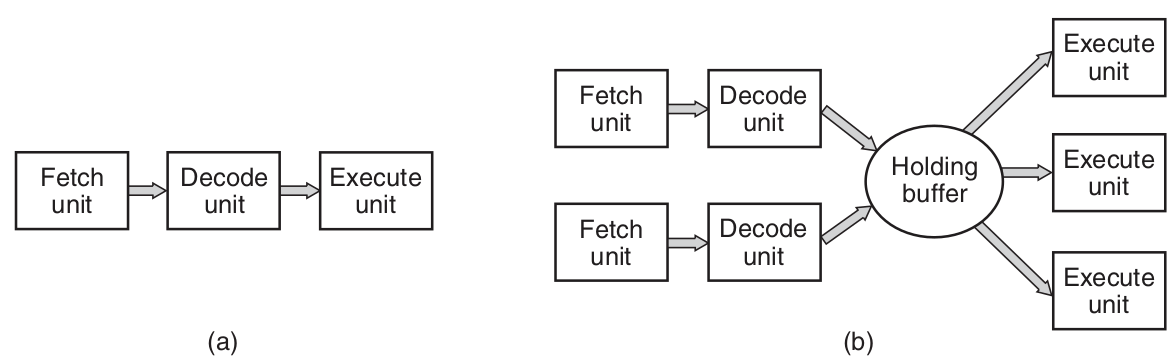
\includegraphics[width=0.75\textwidth]{FIG/1-7.png}
		\caption{一个三阶段的流水线和一个超标量CPU}\label{fig:pipeline}
	\end{figure}
	
	比一个流水线设计更为高级的是超标量CPU,如图 \ref{fig:pipeline}(b)所示。在这个设计中,会有多个执行单元,例如,一个是整数运算,一个是浮点数运算,另一个是布尔数字运算。两条或者更多的指令一次被取出,解码并被装入暂存缓冲区中直到他们被执行。当一个执行单元空闲的时候,它就会检查暂存缓冲区去看是否有它可以执行的指令,如果有的话,它将该指令从缓冲区中移除并执行它。这种设计的含义是程序指令经常是乱序执行的。在多数情况下,是由硬件来保证这种运算的结果和顺序执行指令时的结果相同,但是,仍然有部分令人烦恼的情形被强加给操作系统处理。
	
	大多数的CPU,除了一些用于嵌入式系统中的简单的CPU,大部分前面曾经提到过的两种模式:内核态和用户态。通常由PSW中的一位来控制。当运行在内核态时,CPU可以执行它的指令集中的每一条指令,并且可以访问硬件的每一个特征。在台式机和服务器机器上,操作系统通常运行在内核态,可以完全地访问硬件。在大多数的嵌入式系统中,只有一小段程序运行在内核态,操作系统剩余的部分运行在用户态。
	
	用户程序总是运行在用户态的,它只允许指令集中的一部分指令和硬件的部分特征被访问。通常情况下,所有涉及到I/O操作和内存保护的指令在用户态都是不被允许的。当然,设置PSW的控制位使进入内核态也是不被允许的。
	
	为了从操作系统获取到服务,用户程序必须通过系统调用(System Call)使得程序进入内核态并唤醒操作系统。TRAP指令完成从用户态到内核态的切换,同时启动操作系统。当这个工作完成的时候,控制权在系统调用之后的指令被返回给用户程序。我们将在本章的后续部分详细讨论系统调用的机理。暂时地,我们可以把它理解为一种可以使得操作系统从用户态进入和内核态的一种特殊程序。在排版方面,我们使用小写的Helvetica字体来在后续的文本中表示系统调用,例如:read。
	
	有必要强调的是,计算机使用陷阱而不是一条固定的指令来执行系统调用。大多数的陷阱是由硬件触发来对一些异常的情况发出警告,如除0和浮点数溢出等。在这些情况下,操作系统都得到完全的控制权并决定如何处理这些情况。有的时候,程序必须以一个错误状态终止,有的时候,则可以忽略错误(如对于下界溢出数可以设置为0)。最后,当程序预先声明要处理一些特殊情况时,可以将控制权交还给应用程序让其处理相关情况。
	
	\textbf{多线程和多核芯片}
	
	摩尔定律指出芯片上的晶体管数量每18个月会翻倍,这个定律并不是物理学上的诸如动量守恒之类的定律。而是Intel公司的联合创始人Gordon Moore的一个观察:在半导体公司的处理器工程师们可以以多快的速度缩减晶体管的数量。摩尔定律已经生效了将近30年,而且还有望至少再继续生效10年。到那个时候,每个晶体管的原子数目就会变得非常少,量子力学将会扮演主要的角色,这将限制晶体管数量的进一步缩小。
	
	大量地使用晶体管导致了一个问题,如果处理它们呢?我们看到了一个方法:带有多个功能单元的超标量体系结构。但是随着晶体管的增加,更多的晶体管也是有可能的。一个显然可以做的事情是在CPU芯片上放置更大的Cache,人们肯定会这么做,然后,原先获得的有用效果将最终消失。
	
	一个明显的步骤是不仅只复制功能单元,同时还复制一些控制逻辑。Intel奔腾4处理器中发布了这个属性,称为多线程或超线程,X86处理器以及一些其他的处理器使用了这个属性,如SPARC,Power5,Intel Xeon以及Intel Core系列的。近似地说,多线程是使得CPU保持两种不同的线程状态,并且能在纳秒级的时间内这两个状态之间进行切换。(线程是一种轻量级的进程,或者说是一个运行程序,我们将在第二章进行详细描述。)例如,如果一个进程需要从内存中读取一个字(需要花费多个时钟周期),则一个多线程的CPU就可以切换到另外一个进程,多线程并不提供真正的并行性。在某一个时刻只能有一个进程进行,只不过是线程切换的时间降到了纳秒级别。
	
	多线程对于操作系统而言是有意义的,因为每一个线程对于操作系统而言都像是一个独立的CPU。考虑一下实际有两个CPU的系统,每个系统有两个线程,操作系统将把它视为4个线程。
	
	除了多线程,许多的CPU芯片拥有四个、八个甚至更多的处理器和核心。图 \ref{fig:quadcores} 所示的多核芯片有效地搭载了四个子芯片,每一个子芯片都有自己独立的CPU(关于cahce后面再讨论)。有一些处理器,像Intel Xeon Phi和Tilera TilePro,已经可以在一个芯片上支持60多个核心了。为了充分利用这些多核芯片最终需要一个面向多处理器的操作系统。
	
	顺便说一句,就绝对数量而言,没有什么可以和现代GPU(图形处理器)相比,GPU是一种带有成千上万个微核的处理器,它们擅长处理大量的并发的简单计算,比如在图像应用中渲染多边形,它们不太擅长串行的工作,而且很难编程。尽管GPU对操作系统来说是有用的(加密或者处理网络拥塞),但是并不意味着操作系统本身可以运行在GPU上。
	
	\begin{figure}[ht]\small
		\centering
		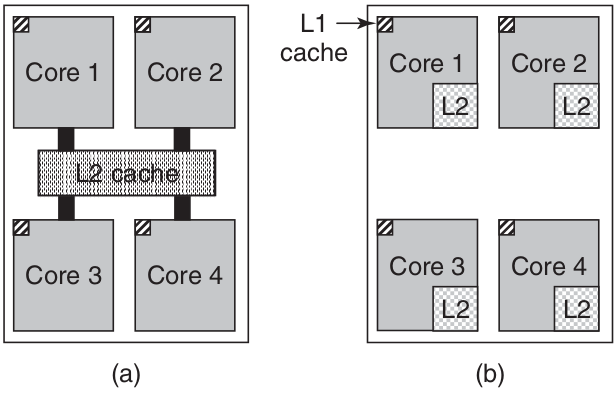
\includegraphics[width=0.75\textwidth]{FIG/1-8.png}
		\caption{一个四核的芯片共享一个L2缓存,一个四核的芯片每核带有独立的L2缓存}\label{fig:quadcores}
	\end{figure}
	
\subsection{内存}

	对于任何计算机而言第二重要的部件是内存。理想情况下,内存应该非常快(甚至比执行一条指令还快,这样CPU就不会被内存掣肘了),非常大而且非常便宜。现有的技术还不能满足以上这些目标,因此采取了另一个方法。内存系统是分层构造的,如图 \ref{fig:memoryhierarchy} 所示。上面的层次拥有比下面层次更快的速度,更小的容量和每字节更贵的价格,其差别往往是十亿数量级甚至更多。
	
	顶层是由在CPU内部的寄存器组成的,他们和CPU相同的材料组成,因此和CPU的速度一样地快。因而,CPU访问它们就不会有什么延迟,他们,它们的典型的存储容量配置是,对于32位的CPU是32 $\times$ 32位,对于64位的CPU是64 $\times$ 64位,都是小于1KB的。程序必须以软件的形式管理这些寄存器(决定把什么东西放进来)。接下来就是缓存内存,几乎是被硬件控制的。主内存被分割为缓存线,典型的是64字节,在缓存线0中的地址是0到63,在缓存线1中的地址是64到127,以此类推。最经常用到的缓存线会被存放到一个高速缓存区,其在CPU的内部或者离CPU非常近的地方。当程序需要读取一个内存字的时候,缓存硬件将会检查所需要的缓存线是否在缓存中。如果在,则称为缓存命中,请求直接在缓存区中得到满足,而不需要通过总线向主内存中发送内存请求。缓存命中通常会占用两个时钟周期,缓存没有命中则必须要到主存中请求数据,将会有巨大的时间代价。缓存的大小通常是受限制的,因为它的成本很高。有一些机器会有两层甚至三层的缓存,每一层都会比上一层空间更大,速度更慢。
	
	\begin{figure}[ht]\small
		\centering
		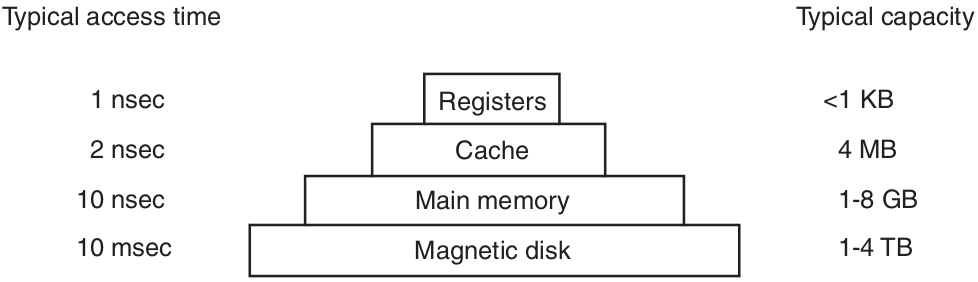
\includegraphics[width=0.75\textwidth]{FIG/1-9.png}
		\caption{一个典型的存储器层级,其中的数据均为粗略值}\label{fig:memoryhierarchy}
	\end{figure}

	缓存在计算机科学的许多领域中发挥着重要的作用,而并不仅仅是RAM的缓存。只要一种资源可以被分成许多的片,其中的一些比另外的一些使用地更加频繁,缓存都经常被用来改善性能。操作系统总是无时无刻不在使用缓存。例如,大多数的操作系统将经常使用的文件存放在主存中以避免经常重复从磁盘中读取这些文件。相似地,将类似「/home/ast/projects/minix3/src/kernel/clock.c」的长路经名转化为文件的磁盘地址可以被缓存下来,以避免重复地查找。最后,当一个网页的地址被转换为网络地址(IP地址),结果就可以被缓存起来供日后使用,还有很多其他应用实例。在任何缓存系统中,一个问题都是很快将会面临到的,包括:
	1. 什么时候向缓存中放入一个新的项目。 
	2. 新的项目放到哪一个缓存行中。
	3. 当需要一个空槽的时候,将哪一个项目移除缓存行。
	4. 将一个刚刚从缓存中移除的项目放到更大内存的什么位置。
	
	并不是每一个问题都会和每一个缓存情形相关。对于在CPU缓存中的主内存缓存行,通常在每次缓存未命中的时候都会进入一个新的缓存行。被使用的缓存线通常是通过被引用内存的高位来计算的。例如,对于64字节的4096缓存行以及32位地址,从第6位到第17位用来标识缓存行,第0位到第5位是在缓存行内部的。在这种情况下,要移除的缓存行可能和新的数据项一样,但是在其他系统中可能不是这样。
	最后,当一个缓存行被写到主内存中的时候(如果它在被缓存后有被修改过),被重写到内存中的地址则是由具体问题中的地址决定的。
	
	缓存是一个如此好的方法以至于现代的CPU都有两个缓存。第一层的缓存或者称为L1 Cache总是在CPU内部,总是解码指令到CPU的执行引擎中。大部分芯片对经常使用的数据字是有一个二级的L1 Cache,大部分的L1 Cache的大小是16KB。除此之外,还有一个经常使用的二级缓存,我们称为L2 Cache,在最近使用的内存字上通常有几MB的内容。L1缓存和L2缓存的区别之处是他们的时间。访问L1缓存是立即无延时的,访问L2级缓存则要延迟1-2个时钟周期。
	
	在一个多核的芯片中,设计者必须自己决定在那里放置缓存。在图 \ref{fig:quadcores} 中, 一个L2缓存是被所有的核心共享的。这个方法应用在Intel的多核芯片中。对比之下,图 \ref{fig:quadcores} 中显示的,每一个核心都有自己的L2缓存,AMD采用了这种方法。每一个策略都有自己的优点和缺点。例如,Intel共享L2级缓存需要一个更为复杂的缓存控制器,AMD采用的方法使得维持L2缓存的一致性更加地困难。
	
	在图 \ref{fig:memoryhierarchy} 中所示的层级结构中,接下来的一级是主存,这是内存系统的主力。主存通常又称为随机访问内存。过去又称为磁芯存储器,因为在20世纪50到60年代,使用小的可磁化的铁磁体来制造主存。它们已经绝迹了很多年,但是名字保留下来了。现在,内存的容量通常是几百MB到几个GB,而且还在快速地增长。所有的CPU的请求,如果缓存中不能得到满足的话,则将会访问内存。
	
	除了主内存外,许多电脑还有少量的非易失性随机访问内存。和RAM不一样的是,非易失性即使是在电源切断的情况下也不会丧失内容。ROM(只读存储器)是在工厂中加工好的,以后就不能再做更改,它速度快而且价格便宜。在一些计算机上,用于启动计算机的引导记载模块就存放在ROM中。而且,还有一些I/O卡采用ROM处理底层设备控制。
	
	EEPROM(Electrically Erasable PROM,电可擦除可编程ROM)和闪存(flash Memory)也是非易失性的,但是和ROM想反,它是可以重复擦写的。但是,擦写它们比写RAM要多花费几个数量级的时间,所以它们和ROM的使用方法一样,而其与众不同的特点是它们可以通过字段重写的方式纠正程序中的错误。
	
	闪存也便携式电子设备中也被广泛地应用。闪存被用于数码相机中的胶卷和便携式音乐播放器中的磁盘,这仅仅是闪存用途中的两项。闪存的速度介于磁盘和RAM之间,但是和磁盘不同的是,如果它被擦写多次的话,它会被写穿。
	
	另外一种类型的内存是CMOS,它是易失性的。许多计算机使用CMOS来保存现在的时间和日期。CMOS内存和增长时间的时钟电路是由一块小电池驱动的,因此,即使是计算机在没有上电运行的情况下,时间也可以被正确地被更新。CMOS内存同时还可以配置参数,如从哪一块磁盘中启动它们。CMOS被使用是因为它耗电很少,即使是使用出厂配置的电池也可以支持好几年的时间。但是,当电池被耗尽的时候,计算机开始呈现出阿兹海默氏症,开始遗忘持续数年的事情,如该从哪个磁盘启动等。
	
	\subsection{磁盘}
	
	在层次图中的下一个层级是磁盘。磁盘存储与内存存储相比,每一位要便宜两个数量级。同时,容量也要大两个数量级。唯一的问题是,它的随机访问数据的速度比内存要慢三个数量级。原因是,磁盘是一个机械设备,其结构如图 \ref{fig:disk} 所示。
	
	\begin{figure}[ht]\small
		\centering
		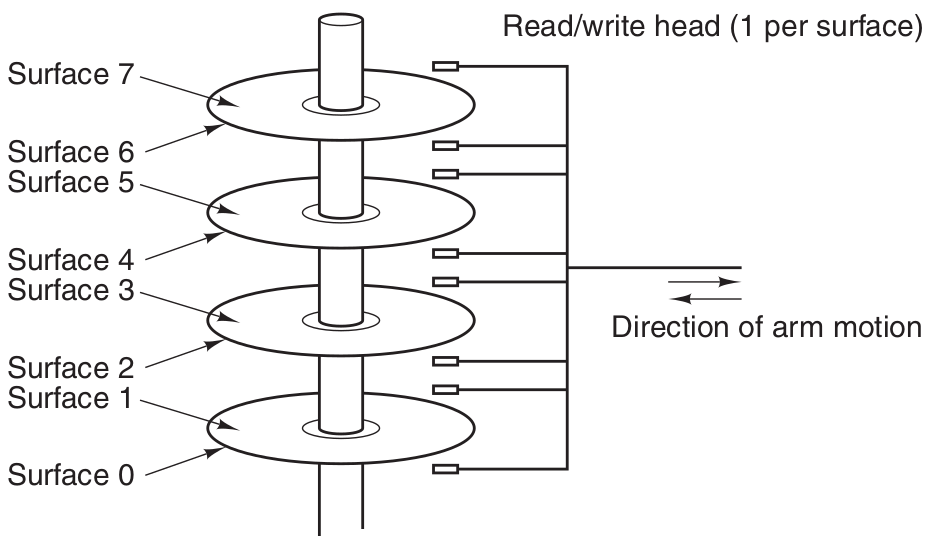
\includegraphics[width=0.75\textwidth]{FIG/1-10.png}
		\caption{一个磁盘驱动器的结构}\label{fig:disk}
	\end{figure}

	一个磁盘是由一个或多个每秒钟旋转5400转,7200转或者10800转的金属盘片组成的。一个机械臂从角落旋转到碟片上,类似于播放塑料唱片的老式33转/分留声机上的拾音器臂。
	
	信息被写道磁盘一系列的同心圆上,对于任意给定的磁盘位置,每一个磁头都可以读取一段环形区域,称为磁道(track)。把一个给定臂位置的所有磁道合并起来,组成一个柱面(cylinder)。
	
	每个磁道被分为若干个扇区,每一个扇区的典型大小是512字节。在现代磁盘中,外部的柱面比内部的柱面包含更多的扇区。将机械臂从一个柱面移动到另一个相邻的柱面大约需要1毫秒的时间,移动到一个随机的柱面大约需要5到10毫秒的时间,具体的时间取决于具体的磁盘驱动器。当扇区移动到相应的磁头下时,则开始读写,低速磁盘的速度为50MB/s,高速磁盘的速度为160MB/s。
	
	有时,你将会听到有人谈论实际上不是磁盘的磁盘,比如固态硬盘(SSD)。固态硬盘并没有可以移动的部分,也不包括像磁盘一样的盘片,它们是把数据存放到闪存中的。与磁盘的唯一相似之处是它们也存储了即使是关闭电源也仍然会保存的大量的数据。
	
	许多计算机支持一种称为虚拟内存(Virtual Memory)的机制,我们将在第三章中使用一定的篇幅介绍它。这种方法使得通过将它们放到磁盘上并且使用内存将最近经常使用到的部分缓存起来的方法来运行比主内存大的应用程序成为了可能。该方案需要动态地重新映射内存地址,将程序生成的地址转换为RAM中字所在的物理地址,这种映射是由CPU的一部分MMU部件完成的。
	
	缓存和MMU的出现会对性能产生很大的影响。在一个多道程序系统中,从一个程序切换到另一个程序称为上下文切换,这个过程需要刷新缓存中所有的被修改块和改变MMU中的映射寄存器。这两个操作的代价都很昂贵,程序员们非常努力地去避免他们。我们稍后将看到他们的战术的一些含义。
	
	\subsection{I/O设备}

	CPU和内存并不仅仅是操作系统所必须管理的资源。I/O设备也和操作系统有着很频繁的交互。就像图 \ref{fig:components} 所示的那样。I/O设备通常包含两个部分:控制器以及设备本身。控制器是一个或者一组物理性的控制设备的芯片。它从操作系统接收命令,例如,从设备中读取数据以及把它们取出。
	
	在大多数情况下,对于设备实际的控制是复杂的和充满细节的,因此控制器的工作是向操作系统提供一个更加简单的接口(事实上,仍然很复杂)。例如,一个磁盘控制器可能会收到一个从磁盘2读取11206扇区的命令。控制器必须将这个线性的扇区数转化为一个具体的柱面、扇区和磁头。这种转化可能会因为下面的情况而变得复杂:外部的柱面比内部的柱面拥有更多的扇区,一些坏的扇区必须被映射到其他的柱面上去。接着控制器必须决定悬臂放在哪一个柱面上,并且给它移入或者移出必须的柱面数的一个命令。它必须等到合适的扇区在磁头下旋转,然后开始读取和存储从驱动器上下来的位,去掉前导码并计算校验和。最后,它们必须将输入的比特组合成单词并把它们存放到内存中。为了完成这些工作,控制器经常包含一些小型的计算机来编程完成它们的工作。
	
	另外一部分是设备本身。设备拥有非常简单的接口,即是因为它们不能做太多的事情同时也是因为要将它们标准化。后者是十分重要的,这样所有的SATA磁盘控制器都可以处理SATA的磁盘。例如,SATA代表串行的ATA,而且ATA则是代表高级技术附件。如果你对AT代表什么表示好奇,它是IBM公司的"第二代个人电脑先进技术",它是1984年基于当时非常强大的6MHZ 80286处理器制造的。从中我们可以看出,计算机有着不断地用新的前缀和后缀来扩展首字母缩写词的习惯。我们还能看出,像“高级”这样的形容词应该谨慎使用,不然30年以后会显得非常可笑。
	
	SATA目前是许多计算机上的标准磁盘类型。因为真正的设备接口隐藏在控制器背后,所有的操作系统可见的是控制器的接口,这个接口可能和设备接口有着很大的区别。
	
	因为控制器的每一个类型都是不同的,每一个都需要不同的软件来进行控制。和控制器交互的软件,给控制器命令并且接收反应,称为一个设备控制器。每一个控制器厂商必须提供一个它所支持的操作系统的驱动。因此,一个扫描仪可能有OS X,Windows 7,Windows 8和Linux等不同的驱动。
	
	为了可以被使用,驱动程序必须被放到操作系统内部,这样他可以运行在内核态。驱动也可以运行在内核外部,像当前的类似Windows和Linux的操作系统也会提供一些类似的支持。绝大多数的驱动程序仍然运行在内核边界以下,只有很少的操作系统MINIX3,则在用户态运行所有的程序。运行在用户态的驱动程序必须被允许以一种受控的方式访问硬件,这种方式是不直接的。
	
	驱动程序被放入内核中可以有三种方式。第一种方式是将新的驱动程序重新连接到系统上并重启计算机,许多旧的UNIX系统是这样工作的。 第二种方法是在操作系统文件中输入一个条目,告诉它需要驱动程序,然后重新启动系统。在启动的时候,操作系统发现它所需要的驱动程序并加载它们,Windows就是通过这种方式工作的。第三种方法是让操作系统在运行时接受新的驱动程序,并且在不需要重新的情况下动态地安装他们。这种方式过去很少见,但是现在已经很普遍了。热插拔的设备,像USB和IEEE 1394设备,也同样需要动态地加载驱动。
	
	每一个控制器都有一小组与之交互的寄存器。例如,一个mini的磁盘控制器应该有识别磁盘地址、内存地址、扇区数、方向的寄存器。为了激活控制器,驱动程序从操作系统中获取一条命令,然后将其转换成适当的值写入设备寄存器。所有设备寄存器的集合构成了I/O端口空间,我们将在第5章中讨论这个主题。 

	在一些计算机中,设备寄存器被映射到操作系统的地址空间中去了,所以它们可以像普通的内存字一样进行读和写。在这些计算机上,无需特殊的I/O指令,用户程序可通过不将这些内存地址放在其可及范围内而远离硬件(通过使用基寄存器和限位寄存器)。 
	
	在其他的计算机上,设备寄存器都被放到一个特殊的I/O端口空间,每一个寄存器有一个端口地址。在这些机器中,提供在内核态使用的专门的IN和OUT指令,供设备驱动程序读写这些寄存器使用。
	前一种方法消除了对特殊指令的需要,但是很占用一些空间,后一种方法不使用地址空间,但是需要一些特殊的指令。两个系统目前都被广泛地使用着。
	
	实际输入和输出的方式有三种。在最简单的方式中,一个用户程序发起一个系统调用,内核将他们翻译成一个驱动设备程序的过程调用。然后,驱动程序启动I/O,并在一个紧密的循环中不断地轮询设备,看它是否完成了(通常有一些位表示设备仍在忙)。然后操作系统将控制权返回给调用者,这种方法被称为忙等待,它的缺点是占用了CPU的轮寻设备直到它完成。当I/O操作完成的时候,驱动程序将数据放置到它们需要的地方并返回。
	接着操作系统将控制权返回给调用者。这个方法被称为忙等待,其缺点是要占据CPU,CPU一直轮询设备直到对应的I/O操作完成。
	
	第二种方法是让驱动程序启动设备,并在完成的时候发出一个中断。设备驱动程序在这个时刻返回。操作系统紧接着阻止调用者并寻找其他工作来做。当控制器检测到传输结束时,它生成一个中断信号来完成。
	
	中断对于操作系统而言非常地重要,因此让我们多探讨一下它。图 给出了一个三步处理I/O的过程。在步骤1中,驱动程序告诉控制器
	接着控制器将启动该设备。当控制器已经结束要它传输的字节数的读或者写,在步骤2中,它使用某些总线线路向中断控制器芯片发送信号。
	如果中断控制器准备好接受中断(如果它正忙于处理一个高优先级的中断,则可能不是这样),则在步骤3中,它断言CPU芯片上的一个pin告诉它。
	在步骤4中,将设备的编号放在总线上,这样CPU可以读取它并知道哪个设备刚刚完成(许多设备可能同时运行)。 
	
	\begin{figure}[ht]\small
	 	\centering
	 	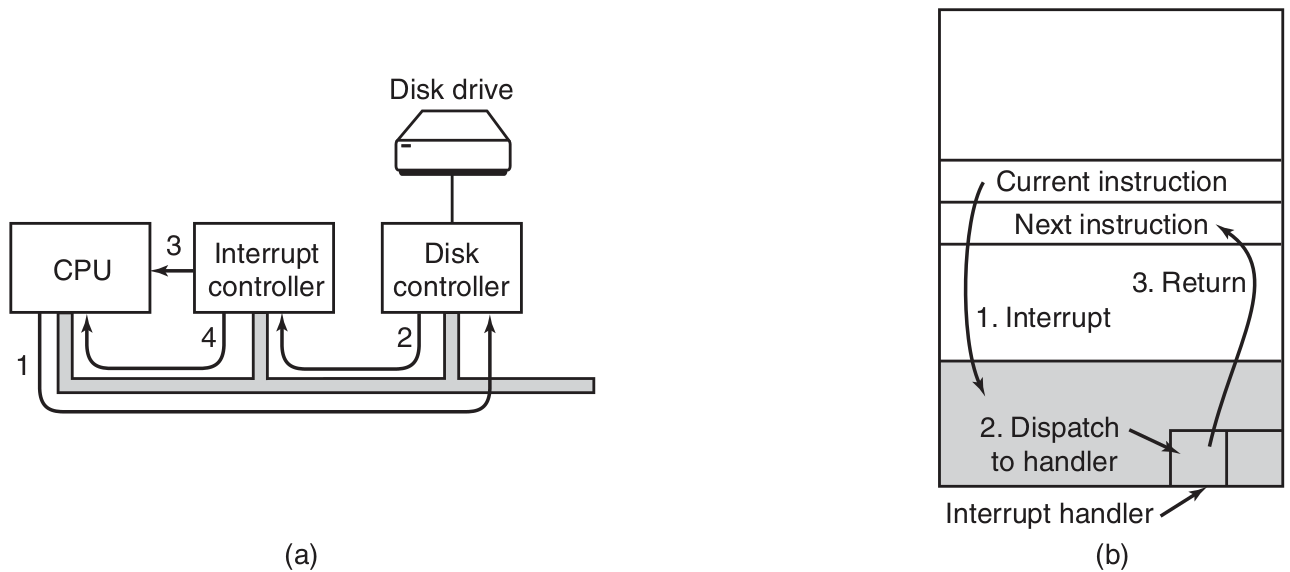
\includegraphics[width=0.75\textwidth]{FIG/1-11.png}
	 	\caption{a. 开启一个I/O设备并获得一个中断,b. 中断处理包括接受中断、运行中断处理程序并返回到用户程序。}\label{fig:interrupt}
	\end{figure}

	当CPU决定处理中断的时候,程序计数器和程序状态字通常会被压入到现在的堆栈中并且CPU被切换到内核模式。设备号可用作内存部分的索引来查找此设备的中断处理程序的地址。这部分的内存被称为中断向量。当中断处理程序(中断设备的部分处理程序)启动后,它移除堆栈程序计数器和PSW并保存他们,接着查询设备获得它的状态。当处理程序全部完成时,它返回到先前运行的用户程序,返回到尚未执行的第一条指令,步骤如图\ref{} 所示。
	
	第三种进行I/O的方法将采用特殊的硬件:一个DMA(Direct Memory Access)的芯片,它可以在不引起CPU干预的情况下控制内存和控制器之间的比特流。CPU安装这个DMA芯片,告诉它传输多少个字节,关联到的设备和内存地址,传输方向等,并且让他离开。当DMA芯片完成后,它将导致一个中断,按上述方法处理。DMA和I/O硬件将在第五章中详细讨论到。因此,CPU有一种方法可以禁用中断,然后在以后重新启用它们。当中断被禁用时,任何完成的设备都会继续断言它们的中断信号,但是直到中断被再次启用,CPU才被中断。如果多个设备在中断被禁用的时候完成,中断控制器决定先让哪一个设备先通过,经常是基于分配给每个设备的静态优先权决定的。拥有最高优先权的设备胜出并且第一个被服务到,其他的设备则必须等待。
	
	\subsection{总线}
	
	图 \ref{fig:components} 所示的组织结构在小型计算机以及最初的IBM PC上被使用了好多年。然而,随着处理器和内存变得越来越快,单个总线处理处理所有流量的能力达到了极限,必须要采取一些措施了。结果,额外的总线被增加了,同时对I/O设备和CPU对内存的速度都更快。这种演化的结果是,一个大型的X86系统看上去像现在图 \ref{fig:x86} 的样子。

	\begin{figure}[ht]\small
		\centering
		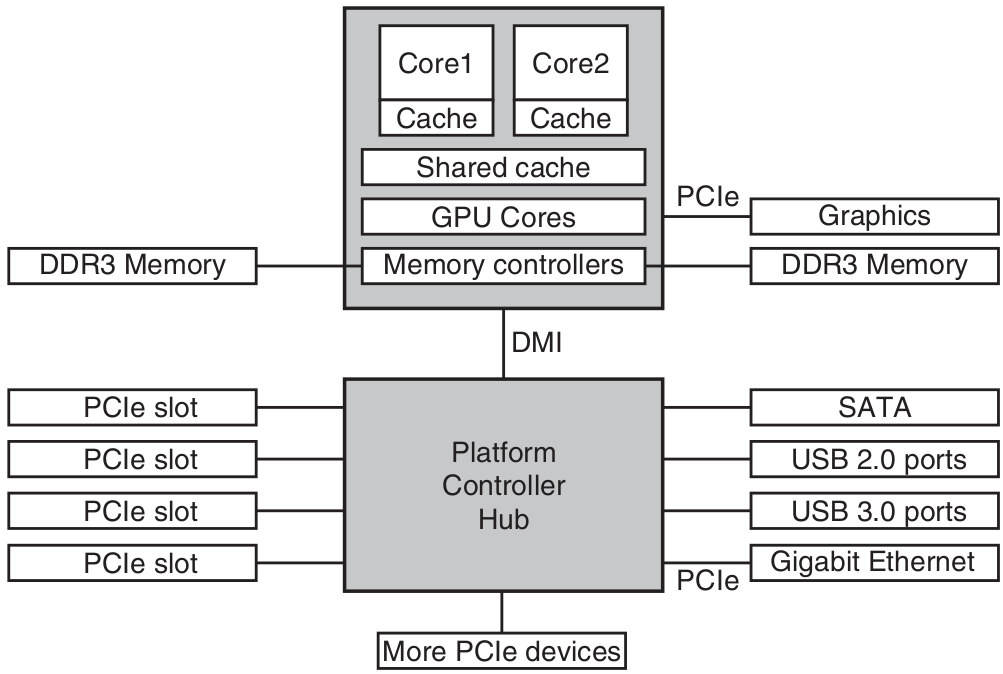
\includegraphics[width=0.75\textwidth]{FIG/1-12.png}
		\caption{一个大型X86系统的架构}\label{fig:x86}
	\end{figure}

	这个系统拥有很多的总线(像cache,memory,PCIe,PCI,USB,SATA和DMI),每一个都有不同的传输速率和功能。操作系统必须对它们进行配置和管理,主要的总线是PCIe(Peripheral Component Interconnect Express)总线。
	
	PCIe总线是Intel发明的作为更旧的PCI总线的一个后继者。PCI总线则是为了取代原来的ISA总线。每秒钟可以传输数十Gb的数据,PCIe比其前代的总线要快很多。它们在本质上也有很多的不同。直到发明PCIe总线的2004年,大多数的总线是并行和共享的,一个共享的总线架构意味着多个设备使用一条线来传输数据。因此,当多个设备都需要传输数据时,你需要一个仲裁者来决定谁可以使用总线。PCIe则恰好相反,它使用分离的,端到端的连接。例如,在通常的PCI总线上,一个32位的数字是通过32个并行的线传输的。和这个不同的是,PCIe使用串行总线架构并且通过一条被称为数据通路的链路传递集合了所有位的一条消息,这非常像网络包。这就简单了很多,因为你就不需要保证32位的数据在几乎相同的时间到达目的地。通过多个数据通路并行起来,并行性仍可以有效利用。例如,我们可以使用32个数据通路并行传输32条消息。随着像网卡和图形适配器等外部设备的速度快速地增加,PCIe的标准每3-5年就会更新一次。例如,PCIe 2.0规格的16个数据通道提供每秒64Gb/s的速度,升级到PCIe 3.0后速度会提升一倍,升级到PCIe 4.0后速度又会提升一倍。
	同时,我们还有很多符合老的PCI标准的旧设备。就像我们在图 \ref{fig:x86} 看到的一样,这些设备被连接到一个独立的集成处理器上。未来,当我们认为PCI不仅仅是“陈旧”,而且是“古老”的时候,很可能所有的设备将连接到另一个集成中心,这些中心再连接到主集成中心,从而形成一个总线树。
	在这种配置下,CPU通过一个快速的DDR3总线与内存进行交互,通过PCIe连接到外部图形设备,通过DMI(直接媒体接口)总线通过集线器连接到所有其他设备。集线器再连接到其他所有的设备,使用统一串行总线连接其他的USB设备,SATA总线连接磁盘和DVD设备,通过PCIe传输以太网络帧。我们已经提到了使用传统PCI总线的PCI设备。不仅如此,每一个核都有自己独享的一个缓存和一个更大的共享的缓存,每一个缓存都会引入一个总线。
	USB总线被发明用来将所有的低速的外部设备与计算机连接,像键盘和鼠标。然而,以5Gb/s运行的设备被认为很慢,这对于伴随第一代以8-Mbps的ISA总线为主要总线的IBM PC机长大的人们来说似乎并不自然。USB使用一个有4到11根线的连接器,有一些线是向USB设备提供电源的或者是地线。USB是一种集中式的总线,其根设备每1ms轮询一次所有的I/O设备看是否有信息收发。USB1.0可以处理总计12Mb/s的负载,USB2.0可以提速到480Mb/s,USB3.0则可以达到不小于5Gbps的速率。任何的USB设备都可以连接到计算机并且不需要重启计算机就可以立即工作,而不像之前的其他设备一样需要重启,这让一批沮丧的用户感到非常惊讶。
	SCIS(Small Computer System Interface)总线是专门为快速磁盘,扫描仪以及其他需要相当带宽的设备所设计的高性能总线。现在,我们经常可以在服务器和工作站中发现它们的身影,它们的速度可以达到640MB/s。
	要想在图 \ref{fig:x86} 所示的环境中工作,操作系统必须知道有哪些外部设备连接到了计算机并且对它们进行配置。这种需求导致了Intel和微软设计了一种即插即用的计算机系统,基于第一次在苹果的Macintosh上实现的一个类似概念。在即插即用之前,每一个外部设备有一个固定的中断请求级别和用于其I/O寄存器的固定地址。例如,键盘的中断请求级别是1,并使用0x60到0x64的I/O地址。软盘控制器的中断等级是6并使用0x3F0到0x3F7的地址,打印机的中断等级是7并使用0x378到0x37A的I/O地址,等等。
	到目前为止,一切正常。但是,当用户买了一块声卡和一块调制解调器,并且都使用中断4的时候,就会产生冲突而不能在一起工作,这个时候问题就产生了。解决方案是像每一个I/O卡上添加DIP开关和调节器,并且指导用户在系统中设定并选择一个不与其他设备冲突的中断等级和I/O设备地址。那些热衷于复杂PC硬件的十几岁的青少年可以不出差错地进行这项工作,而其他人则不能避免出错,这就导致了混乱。即插即用所做的工作是让系统自动地收集I/O设备的信息,集中地分配中断等级和I/O地址,并告诉每一块卡它的号码。这个工作和计算机启动的过程密切相关,所以接下来我们要探讨一下这个过程,这可不是一件轻松的工作。
	
	\subsection{启动电脑}
	
	简单地说,启动过程类似以下过程。每台计算机都有一个双亲板(在政治因素影响到计算机产业之前又叫母板),在双亲板上是一个叫做BIOS的系统程序。BIOS包含低级的I/O软件,包括读取键盘、写屏幕、做磁盘I/O以及一些其他事情的程序。现在,它被保存在一块非易失的Flash RAM中,但是可以在发现bug的时候通过操作系统来修改它。当计算机启动的时候,BIOS就开始工作了。它首先检查计算机中配备了多少内存,并检查像键盘以及一些其他的一些基本的I/O设备是否能够正常地反应。它通过扫描PCIe和PCI总线来开始检查所有与之连接的设备。如果当前的设备和上次系统启动时不一样,则被当作新设备配置。BIOS系统接着通过尝试存储在CMOS内存中的设备列表来决定启动设备。用户可以通过输入一个BIOS的配置程序而在重启之后立即改变这个列表。通常情况下会尝试从CD-ROM或者是USB设备进行启动,如果有一个是可行的话。如果失败了,BIOS则会从硬盘启动。启动设备的第一个扇区会被载入内存并被执行,这个扇区包含一段能够正常检测位于启动扇区尾部的分区表,来决定哪一个设备是活动的,接着从那个分区中读取二级启动加载器,这个加载器从活动分区中读取操作系统并启动它。接着,操作系统将需要BIOS来获取配置信息。对于每一个设备,它检查是否有设备驱动器。如果没有,它将让用户插入一个包含驱动器的CD-ROM(由设备制造厂商提供),或者从网上下载。当它具有所有的设备驱动时,操作系统将它们加载进内核。接着它将初始化表格,创建任何需要的后台线程,启动登录程序或者GUI界面。
	
	\section{操作系统大观园}
	
	操作系统已经存在了半个多世纪。在这段时间里,各种变种都被开发了出来,但是并不是所有的操作系统都很出名。在本节中,我们将讨论它们中的九个。在本书的后面,我们还将回顾一下几种不同的系统类型。
	
	\subsection{大型机操作系统}
	
	操作系统的高端是用于大型机的操作系统,它们是有房间大小的计算机仍然可以在大型公司的数据中心中看到。这些计算机不同于个人计算机在于它们的I/O容量。一个拥有1000块磁盘和数百万GB数据的大型机器是不罕见的,但是如果一台个人计算机拥有这个配置则会让朋友们很羡慕。大型机也在一些高端的网络服务器,大型电子商务网站的服务器,以及B2B业务中有一定的卷土重来。大型机的操作系统主要面向一次性处理很多工作的场景,他们多数都需要巨大的I/O能力。它们通常提供三种典型的服务:批处理、事务处理和分时。一个批处理系统是一个没有和现有用户交互的循环作业的过程。保险公司的索赔处理和连锁店的销售报告通常采用批处理的方式进行。事务处理系统处理大量的小的请求,例如,银行的支票处理和航班预订。每一个工作都很小,但是系统必须每秒种处理成百上千个这样的请求。分时系统允许多个远程系统同时在计算机上作业,如查询一个大型的数据库。这些功能是密切相关的,大型机操作系统通常完成所有这些功能。一个大机操作系统的例子是OS/390,是OS/360系统的后继版本。但是,大型机操作系统逐渐被诸如Linux的这类UNIX的变体所代替。
	
	\subsection{服务器操作系统}
	
	下一个层次是服务器操作系统。它们在服务器上运行,服务器可以是大型的个人机、工作站甚至是大型机。它们通过网络服务多个用户,并且允许用户共享硬件和软件资源。服务器可以提供打印服务,文件服务,Web服务等。Internet提供者运行很多的服务器机器来为消费者服务,网站使用服务器来存储它们的网页并处理来到的请求。典型的服务器操作系统有Solaris,FreeBSD,Linux和Windows Server 201x。
	
	\subsection{多处理器操作系统}
	
	目前获得大量联合计算能力的主要方式是将多个CPU连接到一个系统中。取决于他们是如何连接的以及共享了什么,这些系统被称为并行计算机,多计算机以及多处理器。他们需要专门的操作系统,但是经常是服务器操作系统的变种,配有通信、连接和一致性等专门功能。
	随着个人计算机多核芯片的出现,即使是传统的台式机或者笔记本都开始需要处理小规模的多处理器,而且核心数随着时间的增加而不断增加。幸运的是,由于先年的研究,已经具备了多处理器操作系统很多的知识,因此在多核系统中使用这些知识不是难事,难的是应用程序能够充分地利用这些计算能力。许多流行的操作系统,像Windows和Linux,都是运行在多核上的。
	
	\subsection{个人计算机操作系统}
	
	接下来的类别是个人计算机操作系统。现代的个人操作系统都支持多道程序,经常在启动的时候就有几十个程序开始运行了。它们的工作是对单个用户提供良好的支持。它们被广泛地应用于字节处理、电子表格、游戏及访问因特网等。通常的例子是Linux、FreeBSD、Windows 7、Windows 8和Apple的OS-X。个人计算机的操作系统是如此广为人知,因而不需要怎么介绍。事实上,许多人们甚至都感觉不到其他操作系统的存在。

	\subsection{手持计算机操作系统}
	
	接下来是越来越小的系统,我们来到平板电脑,智能手机以及一些其他的个人电脑。一个手持电脑,以往叫做PDA(个人数字助手),是一个可以在你手中操作的小型计算机。智能手机和平板电脑就是最好的例子。像我们已经看到的这样,现在的市场是由Google的Android和苹果的iOS占据了,但是它们也有很多的竞争者。大部分的这些设备有多核的CPU、GPS、照相机、其他的传感器、大量的内存以及复杂的操作系统。不仅如此,它们都有第三方的应用你可以摇一摇地下载它。	
	
	\subsection{嵌入式操作系统}
	
	嵌入式系统运行的计算机控制那些不被认为是计算机的设备,这些设备不接受用户安装的软件。典型的例子是微波炉、电视、汽车、DVD编码器、传统的电话以及MP3播放器。区别嵌入式系统和手持设备的一个主要特征是,嵌入式系统上不会运行不受信任的软件。你不能为你的微波炉安装一个新的应用程序,因为所有的程序都存放在ROM中。这就意味着操作系统不需要对应用程序进行保护,这就可以带来设计上的简化。系统像嵌入式的Linux、QNX和VxWorks都在这个领域比较流行。
	
	\subsection{传感器-节点操作系统}
	
	小型传感器网络被部署用于很多的目的。这些节点是小型的计算机,他们通过一个基站使用无线网络进行通信。传感器网络被用来保护建筑的外围,保卫国防边境线,检测森林火灾,测量温度和预报降水量,收集战场的敌人移动信息等。传感器是一种内置有无线电的电池驱动的小型计算机。它们的电能很有限,并且需要长时间在野外工作,而且通常是在环境恶劣的条件下。网络必须足够健壮以容忍单个节点的失败。随着电池的逐渐耗尽,这种节点会开始增加。每一个传感器电脑都是一个真实的计算机,有CPU、RAM、ROM以及一个或多个环境传感器。它运行一个小的,真实的操作系统,通常是一个事件驱动的,响应外部事件或者基于一个内部时钟进行周期性地测量。它的操作系统要求小和简单,因为节点的内存很小,电池寿命是一个重要的问题。同时,对于嵌入式系统,所有的程序都会被事先加载,用户不会突然启动他们从网上下载的应用程序,这样就使设计变得非常简单。TinyOS是一个广为人知的用于传感器的操作系统。
	
	\subsection{实时操作系统}
	
	另外一种类型的操作系统是实时操作系统,这些系统的特征是将时间作为关键参数。例如,在工业控制系统中,实时计算机需要收集生产过程相关的数据,并控制在工厂中的机器。通常,系统还必须满足严格的最终时限。例如,如果一辆汽车正在装配线上移动,必须在限定的时间内进行规定的操作。例如,如果焊接机器人焊接地过早或者过晚,都会损害汽车。如果动作需要在一个特定的时间(或者特定的时间段)出现,我们就需要硬实时系统(Hard Real-time System)。其中许多在工业过程控制、航空电子、军事等领域都有,以及类似的应用领域。这些系统必须提供绝对的保证,保证在某个特定的时间内会发生某个动作。
	
	一个软实时系统,是一个偶尔错过最后期限的系统,不可取,可接受,且不会造成任何永久性损坏。数字音频和多媒体系统属于这一个类别,智能手机属于软实时系统。有时候,操作系统仅仅是和应用程序相连接的一个库,各个部分必须紧密耦合而且部分与部分之间没有保护,这一类的实时系统是eCos。
	
	掌上,嵌入式系统以及实时系统的分类在一定程度上不少是互相重叠的。几乎所有的系统都具有软实时系统方面的特征。嵌入式系统和实时系统只运行系统设计者放入的软件,用户不能添加他们自己的软件,这样令保护变得更加简单。手持系统和嵌入式系统是专门为消费者设计的,而实时系统更多的是工业应用。不管如何,他们在一定程度上有相通之处。
	
	\subsection{智能卡操作系统}
	
	最小的操作系统运行在智能卡上,它们是一个信用卡大小的带CPU的芯片。它有非常严格的处理能耗和存储空间的限制。其中,有些是由插入读卡器的触点供电,但是非接触式的卡片是感应供电的,这大大限制了它们可以做的事。其中有些智能卡只能处理一个功能,像电子支付,而其他的卡片可以处理多个功能,它们有专用的操作系统。
	一些智能卡是面向Java的,这意味着在智能卡上的ROM有一个JVM的解释器。Java的小程序被下载到卡片上,并且被卡片上的JVM解释器执行。这些卡可以同时处理多个应用程序,从而导致多道程序并且需要去调度他们。当两个或更多的小程序运行的时候,资源的管理和保护也将会变成一个问题,这些问题都应该由卡片上的操作系统来处理。
	
	\section{操作系统概念}
	
	大多数的操作系统提供基本的概念和抽象,像进程、地址空间、文件等,它们是需要理解的核心内容。在接下来的章节中,我们将简单地考察这些基本概念中的一部分,在本书后面的章节,我们还将对其进行详细的讨论。为了解释这些概念,我们会时不时地使用例子,这些例子主要来源于UNIX。相似的例子同样会存在于其他的系统,我们后续会学习他们中间的一部分。
	
	\subsection{进程}
	
	所有的操作系统一个关键的概念是进程。进程就是一个在正执行的程序。伴随每一个进程的是它的地址空间,是一个从0到某一个最大值的内存位置的列表,可以供进程读和写。地址空间包含可执行的程序,程序的数据以及它的堆栈。同时,伴随每一个进程还有一组资源,通常包括寄存器(程序计数器和栈指针),打开文件的列表,突出的警报,相关进程的列表,以及运行程序所需要的其他信息。一个进程就是为了运行一个程序所包含的所有信息的容器。
	
	我们将在第二章中详细讨论进程的概念。不过,对进程建立起直观观念的一个最便利的方法是分析一个多道程序设计系统。用户可能打开了一个视频编辑程序并发出命令要把它转化为某种格式的一小时视频文件(这个过程可能要花费几个小时),接着他就去上网去了。于此同时,一个周期性的检查到来邮件的后台线程也开始运行了。这样,我们就至少有三个活动的线程:视频编辑器、网络浏览器以及邮件接收器。周期性地,操作系统决定停止运行一个进程而开始运行另外一个进程,那大概是因为在过去的一、两秒中,进程已经使用完了分配给它的时间片。
	
	当一个进程暂时被挂起,它在稍后必须将以停止前的状态被重启。这就意味着关于进程的所有信息在进程挂起的时候必须被显式地保存在某个地方。例如,进程可能会同时打开好几个用于读取的文件,同时还有每个文件当前位置的指针(字节数或者下一个将被读取的记录)。当一个进程被暂时挂起的时候,所有的这些指针必须被保存,这样在执行read系统调用重启进程的时候能够读取到正确的数据。在许多操作系统中,关于每一个进程的所有信息,除了它自己的地址空间的内容,都被保存到一个叫做进程表的操作系统表中,是一个结构的数组,每一个元素代表当前存在的一个进程。
	
	所以,一个挂起的进程包括它的地址空间,通常称为核心镜像(为了纪念以前用到的磁芯存储器),以及它的进程表项,包含了它的寄存器的内容,还有一些稍后重启进程时所必须的一些其他选项。
	
	与进程管理相关的关键的进程管理系统调用是那些创建和终止进程的系统调用。我们来考虑一个典型的例子,有一个叫做命令解释器或者shell的进程从终端读取命令。用户仅仅键入了一个要求编译一段程序的命令,shell必须创建一个运行编译器的新的进程。当这个进程完成编译的时候,它再执行一个系统调用终止自己。
	
	如果一个进程可以创建一个或多个其他进程(称为子进程),这些进程可以创建自己的子进程,我们很快就可以建立起类似图 \ref{fig:processtree} 所示的进程树。
	
	\begin{figure}[ht]\small
		\centering
		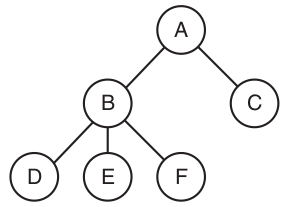
\includegraphics[width=0.75\textwidth]{FIG/1-13.png}
		\caption{一个进程树,进程A创建了两个子进程B和C,进程B创建了三个子进程,D,E和F。}\label{fig:processtree}
	\end{figure}

	相关的进程合作完成一个工作,经常需要和其他进程进行通信并同步它们的行为。这种通信称为进程间通信,我们将在第二章中详细描述。
	其他的进程系统调用可以要求更多的内存(释放没有被使用的内存),等待一个子进程结束,用一个程序覆盖另一个程序。
	
	有时,需要将信息传递给一个正在运行的进程,而该进程并不在等待此信息。例如,一个进程通过计算机网络向另一个远程进程发送消息,通过这种方式和另一台计算机上的进程进行通信。为了防止发送的消息或者它的回复丢失,发送者可能会要求它的操作系统在指定的若干秒后发一个通知,这样如果它还没有收到通知的话就可以重新传送。设置好这个定时器后,程序就可以做其他的工作了。
	
	当指定的若干秒过去后,操作系统向进程发送一个警报信号。这个信号将会导致进程挂起,不管这个进程现在正在做什么,保存它的寄存器在堆栈上,并且开始运行一个特定的信号处理程序。例如,重新传输可能丢失的进程。当信号处理结束的时候,正在运行的进程将会重新从信号之前的状态执行。信号是硬件中断的软件模拟,它可以因为各种原因而产生,除了定时器到期之外。许多陷阱是硬件检测出来的,如执行一个非法的指令或者使用一个非法的地址,也被转换成该信号并转交给这个进程。
	
	每一个使用系统的用户都会被系统管理者分配一个用户ID(UID)。每一个进程都有启动它的用户的UID,子进程和父进程拥有相同的UID。用户可以是组的成员,每个组都有一个组的ID(Group IDentification)。

	有一个UID,称为超级用户(UNIX)或者管理员(Windows),拥有特殊的权力,并且可以违背一些保护规则。在一些大型的安装中,仅仅只有系统管理者只要可以成为超级用户的密码,但是,许多的普通用户(特别是学生),投入了相当多的努力在寻找系统的漏洞上面,从而使他们不用管理员密码也可以称为超级用户。
	
	我们将在第二章讲述进程以及进程间通信。
	
	\subsection{地址空间}
	
	每一台计算机都有一些装载其正在运行程序的主内存。在一个非常简单的操作系统中,在某个时刻只有一个程序在内存中。为了运行第二个程序,第一个程序必须被移除,而把第二个程序放置到内存中。
	
	更多的复杂的操作系统允许多个程序同时驻留在内存中。为了防止他们互相干扰,需要一些保护机制。虽然这个机制是硬件形式的,但是它是被操作系统控制的。
	
	上述管理涉及对计算机主存的管理和保护。一个不同的,但是同等重要的与内存相关的主题是进程地址空间的管理。通常,每一个进程都有一套它可以使用的地址,通常是从0到一个最大值。在最简单的情形下,一个进程地址空间的最大值比主存的大小要小。这样,一个进程就可以填充它的地址空间并且有足够存放它的内存空间。
	
	然而,许多计算机的地址空间是32位或者64位的,地址空间大小分别是2$^{32}$到2$^{64}$字节。如果一个进程有比计算机主存更大的地址空间以及进程想全部使用这些内存的时候该怎么办呢?在早期的计算机中,这样的进程就没那么幸运了。现在,一个被称为虚拟内存的技术存在了,像前面提到的那样,操作系统将地址空间的一部分存放到内存中,一部分放到磁盘中,并且根据需要在它们之间来回穿梭。本质上说,操作系统建立了一个地址空间的抽象,作为进程可以引用的地址集。地址空间从机器的物理内存中被分离出来,并且不是比内存大就是比内存小。对地址空间和内存的管理形成操作系统一个重要的组成部分,我们将在第3章中谈论这个主题。
	
	\subsection{文件}
	
	被所有的操作系统支持的另一个重要的概念是文件系统。像前面提到的一样,操作系统的一个主要功能是隐藏磁盘和其他I/O设备的怪异性,并且呈现给编程者一个友好的、干净的、独立于设备的抽象模型。很明显,创建、删除、读取、写文件都需要系统调用。在读取一个文件之前,必须将它在磁盘上定位并打开,读取完毕之后则需要关闭它,这些都是系统调用做的事情。
	
	为了提供一个放置文件的场所,大多数的PC操作系统都有目录的概念用于将文件组合在一起。一个学生,例如,可能会有一个他正在上的课的目录,一个电子邮件的目录,一个存放万维网主页的目录。系统调用就需要创建和删除目录。系统调用还提供将一个文件放入目录和从一个目录中删除一个文件。目录项可以是文件也可以是其他的目录。这个模型也产生了层次结构-文件系统,像图 所示的那样。
	
	\begin{figure}[ht]\small
		\centering
		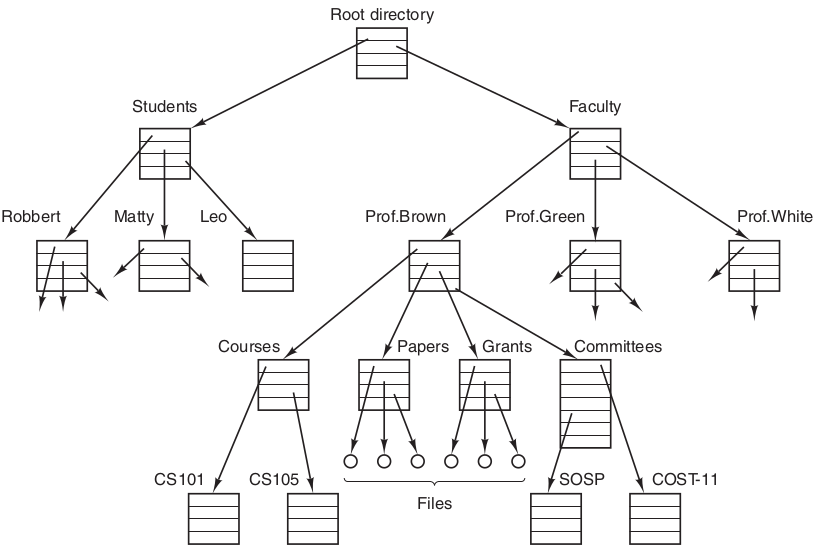
\includegraphics[width=0.75\textwidth]{FIG/1-14.png}
		\caption{一个文件系统的层次结构}\label{fig:fshierarcy}
	\end{figure}
	
	进程和文件层次都是按照树的结构来组织的,但是又有很大地不同。进程树通常不会很深(深过3层就不太正常了),然而文件层次却经常有4级,5级甚至更深。进程的层次通常是短暂存在的,通常最多只有几分钟,而目录层次却可以存在数年之久。进程和文件的所有者和保护机制也有很大不同。典型地,仅仅是一个父进程可以控制和访问一个子进程,但是对于文件和目录而言却需要允许所有者之外的其他很多用户来访问。
	
	目录层次结构中的每个文件都可以通过指定其路径来指定目录层次结构顶部的名称,根目录。这个绝对的路径名包含目录的列表,必须从根目录开始访问来获取这个文件,用斜线分离每一个组件。如图 \ref{fig:fshierarcy} 所示,文件CS101的路径是/Faculty/Prof.Brown/Courses/CS101。最前面的斜线说明该路径是绝对路径,是从根目录开始的绝对路径。顺便提及,由于历史原因,在Windows中,使用反斜线($\backslash$ )来代替正斜线作为分隔符。所以上述的文件路径在Windows下应该是$\backslash$Faculty$\backslash$ Prof.Brown$\backslash$ Courses$\backslash$ CS101。在本书中,我们通常采用UNIX的传统来代表路径。

	在每一个时刻,每一个进程都有一个工作目录,在其中查找不以斜杠开头的路径名。例如,图 \ref{fig:fshierarcy} 中,如果$\backslash$Faculty$\backslash$ Prof.Brown是当前的工作目录,使用路径Courses/CS101将生成与上面给出的绝对路径名相同的文件。进程可以通过发出指定新工作目录的系统调用来更改其工作目录。在一个文件被读和写之前,它必须先被打开,在此时将会检查权限。如果访问被允许了,系统返回一个称为文件描述符的小整数,用于后续操作。如果禁止访问,则返回错误代码。另外在UNIX中的一个重要的概念是挂载文件系统。大部分桌面台式机会有一个或者多个光驱可以插入CR-ROMs,DVDs和镭射光盘。它们也通常有USB接口,可以用来插入USB内存棒(实际上是固态硬盘),还有一些计算机有软盘和外置硬盘。为了提供一个处理这些可移动设备的优雅方法,UNIX允许这些在光盘上的文件系统可以被添加到主目录树上。考虑图 \ref{fig:mounting}(a) 的情形。
	
	\begin{figure}[ht]\small
		\centering
		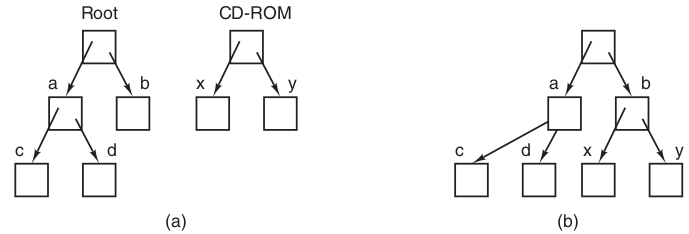
\includegraphics[width=0.75\textwidth]{FIG/1-15.png}
		\caption{(a)在挂载之前,CD-ROM上的文件是不可访问的,(b)挂载之后,它们称为文件目录的一部分。}\label{fig:mounting}
	\end{figure}

	在mount系统调用之前,在硬盘上的根文件系统,以及在CD-ROM上的二级文件系统,是独立的和不相关的。但是,无法使用CD-ROM上的文件系统,因为无法在其上指定路径名。UNIX不允许以设备名称或者设备号为开头作为前缀,这正是操作系统应该消除的对设备的依赖。
	相反,\texttt{mount}系统调用允许CD-ROM上的文件系统在程序想要的任何地方添加到根文件系统。图 \ref{fig:mounting}(b) 中,CD-ROM已经被挂载到目录b中,因此允许访问文件/b/x和/b/y。如果目录b
	包含有任何不能访问的文件而CD-ROM被挂载上了,/b指代的是CD-ROM的根目录。(无法访问这些文件并不像最初看起来那么严重:文件系统几乎总是安装在空目录上。)如果一个系统包括多个硬盘,它们也都可以被映射到一个目录树上。
	在UNIX中,另外一个重要的概念是特殊文件(Special File)。提供特殊文件是为了让I/O设备看起来像文件一样。这样,它们就可以使用同样的系统调用进行读和写,就像读和写文件一样。有两种特殊文件存在:	块特殊文件和字符特殊文件。块特殊文件用于对由随机寻址块(如磁盘)组成的设备进行建模。通过打开一个块特殊文件并且读取它们,例如,块4,程序可以直接访问到块特殊文件的块4,而不需要关心包含它的文件系统的结构。相似地,字符特殊文件用来模拟打印机、调制解调器、以及其他可以接收或输出字节流的设备。通常而言,特殊文件保存在/dev目录下。例如,/dev/lp可能是打印机(曾经称为行式打印机)。
	
	我们在概述中讨论的最后一个特征是同时和进程与文件相关:管道。管道是一种可以用来连接两个进程的伪文件,像图 \ref{fig:pipe} 所示的那样。如果进程A和B想通过管道进行对话,则它们必须事先安装好管道。当进程A想向进程B发送数据的时候,它把数据写在管道上,仿佛管道是一个输出文件。事实上,管道的实现也非常像是一个文件。进程B可以从管道中读取数据就好像读取一个文件一样。因此,UNIX中的进程间通信就非常类似于普通文件的读和写。更强大的是,进程发现它正在写入的输出文件不是一个真正的文件而是一个管道的唯一的方法是使用一个特殊的系统调用。文件系统非常重要,我们将在第四章、第十章和第十一章中详细讨论。

	\begin{figure}[ht]\small
		\centering
		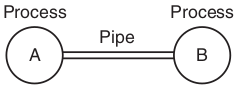
\includegraphics[width=0.75\textwidth]{FIG/1-16.png}
		\caption{连接两个进程的管道}\label{fig:pipe}
	\end{figure}

	\subsection{输入/输出}
	
	所有的计算机都有需要输入和产生输出的物理设备。毕竟,如果用户不能告诉它要做什么以及在做完之后不能得到工作的结果的话,那么计算机又有什么用呢。有许多种输入输出设备的存在,包括键盘、显示器、打印机等等。这取决于操作系统如何管理这些设备。所以,每一个操作系统都有管理其I/O设备的I/O子系统。一些I/O软件是设备独立的,即这些I/O软件部分可以同样应用于许多或者所有的I/O设备上。其他的部分,像设备驱动器,是专门为特定的I/O设备设计的。在第五章中,我们将讨论IO软件。
	
	\subsection{保护}
	
	计算机中包含大量的用户想要保护和设置为隐私的信息。这些信息包括邮件、商业计划、退税等诸多内容。管理系统的安全性完全取决于操作系统,例如,仅对授权用户访问。作为一个简单的例子,考虑一下安全是怎样工作的,请参考UNIX。UNIX中的通过分配给每一个文件9位的二进制保护码来保护文件。保护码包括三个三位的字段,一个用于所有者,一个用于与所有者同组的其他人员,另一个用于其他用户。每一个字段中有一个用于读访问,一个用于写访问,一个用于执行访问。这三个位就是所谓的rwx位。例如,保护码\texttt{rwxr-x--x}意味着所有者可以读、写和执行,同组内的其他成员可以读和执行该文件(但是不能写),而其他用户则只能执行该文件(不能读和写)。对于一个目录,x意味着检索权限,横线表示相应的权限是缺失的,没有的该当权限。除了文件保护之外,还有许多其他的安全问题。保护系统不受不合法的用户,包括人类和非人类(如病毒)的入侵,则是其中之一,我们将在第9章中讨论不同的安全问题。
	
	\subsection{Shell}
	
	操作系统就是一堆执行系统调用的代码。编辑器、编译器、汇编程序、连接程序、功能程序以及命令解释行等尽管它们非常重要,但是它们不是操作系统的一部分。冒着将事物弄得稍微有些复杂的危险,我们在本节中简单地介绍一下UNIX的命令行解释器,Shell。尽管它不是操作系统的一部分,但是它体现了操作系统许多重要的特性,并且很好地说明了系统调用的具体用法。Shell同时也是终端用户和操作系统之间的接口,除非用户正在使用图形用户界面。Shell有很多种,包括sh,csh,ksh和bash。所有的它们都支持下方描述的功能,这些功能可以追溯到早期的shell(即sh)。
	当任何一个用户登录的时候,一个shell程序就启动了。Shell程序有标准输入和标准输出的终端。它首先显示提示符(prompt),一个像美元符号的标识,告诉用户shell现在正在等待接收命令。如果这时候用户键入一个\texttt{Date}命令,shell就会创建一个子进程并且运行date程序。在子进程运行的时候,shell等待它终止。当子进程结束的时候,shell重新输出提示符,并且试图读取下一行。用户还可以将标准的输出重新定位到一个文件,例如:date > file。同样,标准的输入也可以重定向,像sort < file1 > file2,将会启动sort程序,从file1中读取输入,将结果输出到file2中。通过管道,可以将一个程序的输出变成另外一个程序的输入。像cat file1 file2 file3 | sort > /dev/lp,它将file1,file2,file3进行连接,并且将输出发送给sort程序,按照字符顺序对所有的行进行排序。sort程序的输出结果重新定位到文件/dev/lp上,通常是一个打印机。如果用户在命令后加上和号,shell不会等待它完成。相反,它只是立即给出提示符。结果,cat file1 file2 file3 | sort > /dev/lp \& 将会启动sort作为后台程序继续执行,这样将允许用户继续工作而sort程序也可以继续进行。shell还有一些其他很有趣的特征,我们在这里就不一一讨论了。有许多UNIX的书籍详细地讨论了shell(像Kernighan and Pike, 1984; Quigley, 2004; Robbins,2005)。今天,大部分的个人计算机都使用GUI,GUI实际上只是运行在操作系统之上的一个程序,像一个shell。在Linux系统中,这个事实更加明显,因为用户可以在两个GUI程序之间选择一个:Gnome和KDE,或者两个都不选(只是用一个X11的终端窗口)。在Windows中,也可以通过修改注册表中的一些值将标准的Windows桌面(Windows Explorer)改成另外的一个程序,尽管很少有人这么做。
	
	\subsection{胚胎重演律}
	
	在达尔文的《 物种起源 》一书出版以后,德国动物学家恩斯特·海克尔(Ernst Haeckel)说:“个体发育概括了系统发育。” 他这样说是意味着胚胎(个体发育)的发展重复着种群(系统发育)的演化。换句话说,在受孕以后,一个人类的胚胎在变成一个人体之前,经历了鱼,猪等发展阶段。现代的生物学家认为这是一种总体的简化,但是还是包含了内在的真相。在计算机工业也发生了类似的相似性,每一个新的物种(大型机、小型计算机、个人电脑、手持电脑、嵌入式电脑、智能卡)等,都经历了像他的祖先一样的发展历程,不管是硬件方面还是软件方面。我们经常忘记在计算机领域所发生的事情以及其他的很多领域都是技术驱动的。古罗马缺少汽车的原因并不是他们有多么地喜欢走路。而是因为他们不知道如何去建造汽车。个人计算机的存在不是因为数以百万计的人们压抑了数世纪之久的对计算机的渴望,而是因为现在可以很廉价地制造它们了。我们已经忘记了技术对我们的系统的视角影响有多大,这一点值得我们时不时地进行反思。特别的是,技术的改变常常会导致这个想法过时了,很快就消失了。然而,另外一个技术上的变化又可以让他重新复苏。这一点是绝对真实的,当需要对系统不同部分的相对性能而作出改变的时候。例如,当cpu比内存快很多的时候,缓存就变得非常重要来加速"较慢"的内存。如果有一天新的内存技术使得内存比CPU快很多的时候,缓存就会消失了。而如果一个新的CPU技术又比内存快很多的时候,缓存就会再次出现。在生物学中,灭绝是永恒的,但是在计算机技术而言,这些在短短数年之内就有可能发生。因为这种无常性,我们将在本书内经常提到一些"过时"的概念,一些对现有的技术不是最佳的想法。然而,技术上的变化又会使得一些"过时的概念"重新回到人们的视野。因为这个原因,弄清楚技术为什么会过时以及环境中的什么变化中会使得它再次复活就显得非常重要。
	为了更加明晰这一点,让我们考虑一个简单的例子。早期的计算机拥有无法改变的指令集,这些指令直接被硬件执行而且不能被更改。接着就产生了微程序(最初在IBM360机器上大规模引用的),一个底层的解释器用软件的形式解释"硬件指令"。硬连线执行就变得过时了,因为其不够灵活。接下来又发明了RISC计算机,这样微程序又过时了,因为硬件直接执行起来更快。现在我们看到解释执行正在以被发送到网络上在到达的时候解释执行的Java Applet小程序的形式复兴了。执行速度不总是最关键的因为网络延迟如此之大以至于他们往往占据着主导地位。因此,天平已经在直接执行和解释执行之间摇摆了好几个周期,而且未来还有可能会再次摆动。
	
	\textbf{大型内存}
	
	让我们来回顾一下硬件的发展历程以及它是如何影响软件的发展的。第一代的大型机拥有很有限的内存,一个完全配置的IBM 7090或者7094机器,从1959年末到1964年占据了山峰之上王者地位的机器,仅仅只有
	128KB的内存。它主要使用汇编语言编程,它的操作系统主要是使用汇编语言编写的以节约宝贵的内存资源。随着时间的推移,像FORTRAN和COBOL等语言的编译器变得足够好了,以至于汇编语言死亡了。但是,当第一代的商业小型机(PDP-1)发布的时候,它只有4096 18位字节的内存,汇编语言惊奇地杀了回来。最后,小型计算机需要更多的内存,高层次语言又变得流行起来了。
	
	当小型计算机在1980年代问世时,第一代计算机拥有4KB的内存,汇编语言又起死回生了。嵌入式计算机最初也使用和微型计算机一样的CPU芯片(8080s,Z80s和后来的8086s),最初也是在编译器中编程。现在,他们的继承者个人计算机,拥有更多的内存并且使用C,C++,Java和一些其他的高级编程语言进行编程。智能卡也正经历一个类似的发展过程,尽管超过了一定的规模,智能卡通常会有一个Java解释器并且解释性地执行Java程序,而不是让Java被编译成智能卡的机器语言。
	
	\textbf{受保护的硬件}
	
	早期的大型机器,像IBM的7090/7094机器一样,没有受保护的硬件,所以他们只是在一个时间运行一个程序。一个有bug的程序很可能会毁掉操作系统,并且使得整个机器崩溃。随着IBM360机器的问世,提供了保护硬件的原型。这些机器可以同时在内存中保存多个程序,并且让他们轮流执行(多道程序),单道程序就被认为是过时了。至少是到了第一个小型计算机出现时- 还没有保护硬件-这样多道程序就不可能的。尽管PDP-1和PDP-8没有保护硬件,而最终PDP-11有了,这个特征最终导致了多道程序和UNIX的诞生。当第一代微型计算机建造的时候,它们使用Intel的8080CPU芯片,其没有硬件保护,所以我们就回到了单程序编程,在内存中一次运行一个程序。直到Intel 80286硬件芯片,多道程序设计才成为了可能。直到今天,许多嵌入式系统还没有硬件保护而仅仅只是运行一个程序。
	现在我们来看一下操作系统。第一代大型机最初没有硬件保护也不支持多道程序编程,所以他们运行简单的操作系统,一次只能处理一个手动加载的程序。后来,他们获得了硬件和操作系统的支持,可以同时处理多个程序,这样他们一次就只可以手动加载一个程序。接着,他们就要求硬件和操作系统一次性支持和处理多个程序,然后是完全的分时能力。
	
	当小型机器第一次出现的时候,他们也没有保护的硬件,尽管那时多道程序设计在大型机领域已经很成熟了。逐渐地,他们要求硬件保护以及一次性运行两个或多个程序的能力。第一代的微型计算机的出现也可以在一次只运行一个程序,但是后来也要求运行多道程序。手持计算机和智能卡遵循同样的发展道路。
	
	在所有的情形下,软件的发展都是由技术决定的。第一代的微型计算机,大部分有4KB的内存和没有硬件保护。高级语言和多道程序对于这么小的一个系统而言就显得太多了。随着微型计算机演化为现代个人计算机,拥有了必要的硬件,接着开始要求软件开始处理一些高级的特征。这种发展很可能会持续数年。其他领域也可能有这种转世轮回,但在计算机行业似乎转得更快。
	
	\textbf{磁盘}
	
	早期的大型机器主要是基于磁带的。他们将会从磁带中读取程序,编译程序,运行程序并将结果写回到另一个磁带上。那时没有磁盘也没有文件系统的概念。这一切开始改变当IBM在1956年发布了它的第一款硬盘-RAMAC以后。它占据了差不多4平方米的地板面积可以存储500万7位的字符,这足够存储一张中等分辨率的图片。但是年度租金就高达35000美元,比存储占据同样空间数量的胶卷还要贵。不过磁盘的价格最终还是下降了,
	并开始出现了原始的文件系统。这些新开发的典型产品是CDC6600,它于1964年推出,多年来一直是世界上速度最快的计算机。用户可以创建所谓的“永久文件”,方法是给文件命名,并希望没有其他用户也认为“数据”是一个合适的文件名,这是一个单级目录。最终,大型机开发了复杂的分层文件系统,可能最终形成了MULTICS文件系统。
	随着小型计算机开始被使用,它们最终也有了硬盘。PDP-11在它1970年代被发布的时候,搭载的标准硬盘是RK05硬盘,大小为2.5MB,大约为IBM RAMAC硬盘的一半,不过其直径大约为40厘米,高度为
	5厘米。但是一开始也都是一个单层的目录。当微型机器开始出现的时候,CP/M是主流的操作系统,但是也只是在磁盘上支持一个目录。
	
	\textbf{虚拟内存}
	
	虚拟内存机制使得计算机可以运行比实际物理内存大的程序,通过在磁盘与内存之间快速地移动信息块的方式。它经历了一个类似的发展过程,一开始出现在大型机上,后来出现在小型机和微型机上。虚拟内存还允许程序在运行的时候使用动态链接库,而不是做内置编译。MULTICS是第一个这样做的系统。最终,这一思想传播开来并广泛应用于大部分的UNIX和Windows系统中。
	在这些发展中,我们会看到,在一个背景下被发明的东西,在另外一个背景下可能会过时(如汇编语言编程,单道编程,单层目录等),但是在下一个十年后可能又会重新出现。出于这个原因,在本书中,我们有时会看到一些想法和算法,这些想法和算法可能在今天的千兆个人电脑上过时,但很快就会在嵌入式计算机和智能卡上出现。 
	
	\section{系统调用}
	
	我们可以看到,操作系统有两个主要的功能,提供应用程序的抽象和管理计算机的资源。在大多数情况下,应用程序和操作系统之间的交互主要处理前者,例如,创建,写入,读取和删除文件。对于用户而言,资源管理部分主要是透明和自动完成的。所以,用户程序和操作系统之间的接口主要就是处理这些抽象。为了想真正了解操作系统干什么的,我们必须非常仔细地分析这个接口。接口中可用的系统调用因操作系统而异(尽管底层的概念是非常相似的)。我们需要在做出一个选择:(1) 模糊的一般性("操作系统有读取文件的系统调用")和(2) 一些特别的系统("UNIX有一个带有三个参数的系统调用:一个是识别文件,一个是告诉数据放到那里,另一个是读取多少个字节,另一个告诉读取多少个字节。") 我们选择采用后一种方法。尽管这个讨论特指POSIX(国际标准9945-1),以及UNIX,System V,BSD,Linux和MINIX3等,但是多数操作系统都有实现相同功能的系统调用,尽管他们实现的细节有很大不同。由于引发系统调用的机器是非常依赖于机器的,而且必须要以汇编代码表达,所以通过提供过程库使得C程序中可以实现系统调用,当然也包括其他的语言。
	
	记住下列事项是非常有益的。任何一个单CPU的计算机一次都只能执行一条指令。如果一个进程在用户态运行一个用户程序而需要一个系统服务,向从一个文件中读取数据,它需要执行一个trap指令向操作系统转移控制权。然后操作系统通过调查参数来判断进程想要什么。然后它执行系统调用并把控制权返回给系统调用后的指令。在某种程度上,执行系统调用就像是执行一个过程调用,区别仅仅在于系统调用进入内核而过程调用不进入内核。
	为了更加弄清楚系统调用的机制,我们来快速地看一下read系统调用。像前面提到的那样,它有三个参数:第一个参数指定文件,第二个参数指向缓冲区,第三个参数确定要读取的字节数。和所有的系统调用一样,它的调用由C程序通过调用一个同名的库过程read来完成。一个由C程序进行的调用,形式如下:count = read(fd, buffer, nbytes);
	系统调用(和库过程)以数字的形式返回实际读取的字节数,这个值通常和nbytes一样,但是也有可能会小一些,例如,在读取文件的时候遇到了文件的末尾。
	如果系统调用因为无效的参数或者磁盘错误不能被执行,counts的值将被设置为-1,错误号码将会放到一个全局变量中,errno。程序应该检查系统调用的结果,以了解是否出现了错误。
	系统调用是通过好几个步骤来执行的,为了将概念弄得更清楚一些,让我们看一下上面讲到的read系统调用。在准备调用实际启动系统调用的read库过程之前,调用程序首先将参数压栈,如图 \ref{fig:read11steps} 所示。
	
	\begin{figure}[ht]\small
		\centering
		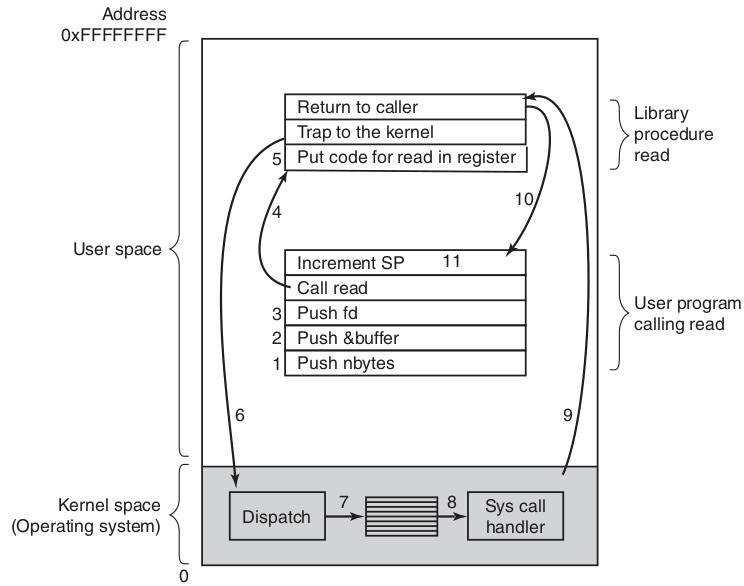
\includegraphics[width=0.75\textwidth]{FIG/1-17.png}
		\caption{调用read系统调用的11个步骤}\label{fig:read11steps}
	\end{figure}
	
	C和C++的编译器由于历史原因将参数以逆序的形式压栈(必须把第一个参数赋给printf(格式字符串),放在堆栈的顶部),第一个和第三个参数是通过值调用的,而第二个参数则是通过引用传递的,意味着缓冲区的地址(由\&指明)传递出去了,而不是缓冲区本身。接下来是真正地调用库过程(步骤4)。此指令是用于调用所有过程的正常过程调用指令。库过程,通常是用汇编语言写的,通常是将系统调用号放到操作系统所期望的一个地方,比如,寄存器中(步骤5)。接着它执行一个TRAP指令,从用户态切换到内核态,并从内核的一个固定地址开始执行(步骤6)。TRAP指令实际上和过程调用指令非常地相似,因为它后面的指令来源于一个遥远的位置,返回地址保存在堆栈上以备以后使用。不管如何,TRAP指令在两点上和过程调用指令不同。首先,是一个副作用,它将切换到内核态。而过程调用指令不改变这种模式。其次,不像给定过程所在的相对和绝对地址那样,TRAP指令不能跳到任意的地址上。根据机器的体系结构,或者跳转到单个固定地址上或者指令中有一个8位长的字段,它给定了内存中一张表格的索引,这张表格中含有跳转地址。
	跟随在TRAP指令后面的内核代码开始检查系统调用编号,并把它分配到正确的系统调用处理器,通常是通过一张由系统调用编号所引用的,指向系统调用处理器的指针表来完成(步骤7)。此时,系统调用处理器开始工作(步骤8)。一旦系统调用处理器完成了其工作,控制可以在TRAP指令之后的指令处返回给用户空间库过程(步骤9)。然后,此过程返回到中的用户程序通常的方法是调用return(步骤10)。为了完成这项工作,用户程序必须清理堆栈,就像它之后做的那样任何过程调用(步骤11)。假设堆栈是往下增长的,它通常情况下确实也是这样的,编译后的代码将堆栈指针的增量精确到足以删除在调用读取之前推送的参数。
	程序现在可以做它任何想做的事情了。
	在上面的9步中,我们提到:"控制可能会返回给用户空间库过程",这是有原因的。例如,如果它试图从键盘读入数据而没有得到任何的输入,那么调用者就必须被阻塞。在这种情况下,操作系统将会看一下有没有其他的进程可以运行。稍后,如果进程获取了想要的输入,进程将会获得操作系统的注意,并开始执行步骤9-11。
	在接下来的章节中,我们将会探讨经常会使用的POSIX系统调用,或者更具体地说,考察这些系统调用的库过程。POSIX大约有100个过程调用,图 列出了其中最重要的一些,为了方便我们把它们分为四类。接下来我们将简要地介绍一下每一个过程调用,以及它们是做什么的。在很大程度上,这些系统调用提供的服务决定了操作系统必须做什么事情,由于个人计算机上的资源管理功能是比较简单的(至少与多用户的大型机相比是这样)。所包含的服务包括创建和终止进程,创建,删除,读取,写入文件,目录管理以及完成输入/输出。值得指出的是,POSIX过程调用和系统调用并不是一对一的。POSIX标准指定了一个符合规范的系统必须提供的许多过程,但是它没有指定它们是系统调用、库调用还是其他什么。如果一个过程可以不执行系统调用而被执行(即可以不陷入内核态),它通常会因为性能原因在用户态执行。而然,大部分的POSIX过程将触发系统调用,经常是一个过程映射到一个系统调用上去。在一些情况下,特别是当几个过程之间只是很细小的区别时,通常是几个过程共同执行一个系统调用。
	
	\subsection{进程管理系统调用}
	
	\begin{figure}[ht]\small
		\centering
		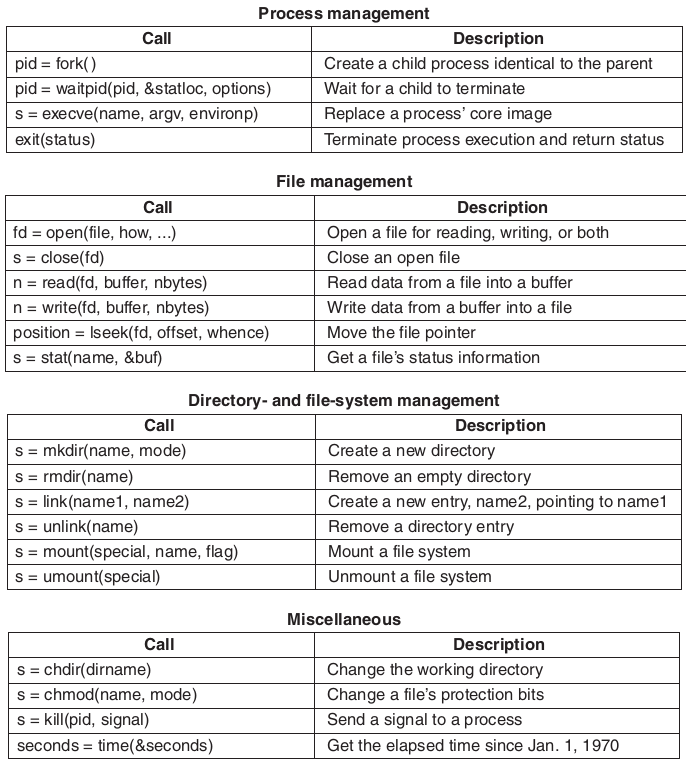
\includegraphics[width=0.75\textwidth]{FIG/1-18.png}
		\caption{一些主要的POSIX系统调用}\label{fig:systemcalls}
	\end{figure}
	
	在图 \ref{fig:systemcalls} 中的系统调用处理进程管理。Fork是一个可以开始讨论的好地方,Fork是POSIX中唯一一个创建新进程的方法。它创建了一个原始进程的精确副本,包括所有的文件描述符,寄存器等一切事物。在Fork之后,原始进程和副本进程各自走自己的路。所有的变量在fork的时候拥有相同的值,但是在父进程的数据完全被复制给子进程后,他们各自的后续变化将不再影响另一个(程序文本,是不可更改的,在父进程与子进程中共享)。Fork系统调用返回一个值,在子进程中是0,在父进程中是PID(Parent IDentifier),使用返回的PID,可以分别出哪一个是父进程,哪一个是子进程。
	在大多数情况下,在fork之后,子进程需要执行和父进程不同的代码,考虑一下shell的情况。它从终端处读取一条指令,派生子进程,等待子进程执行命令,当子进程结束的时候读取下一个指令。为了等待子进程结束,父进程执行一个\texttt{waitpid}系统调用,该系统调用只是等待子进程结束。\texttt{Waitpid}可以等待一个特殊的子进程,或者是任意一个旧的子进程,通过把第一个参数设置为-1。当\texttt{Waitpid}完成后,被第二个参数指向的地址,statloc,将被设置为子进程的退出状态(正常,异常退出和退出值)。通过第三个参数也可以有不同的选项,例如,如果没有子进程退出的话则立即返回。
	现在考虑shell是如何使用fork的,当一个命令被键入的时候,shell调用fork执行一个新的进程,这个子进程必须执行用户指令。通过使用execve系统调用来实现这一点,这将导致整个核心镜像被其第一个参数命名的文件所替换。(事实上,系统调用本身是exec,但是有几个库过程通过不同的参数和不同的名字。我们将在这里处理这些系统调用。) 图 \ref{fig:simpleshell} 是一个高度简化的shell阐述了fork,waitpid和execve是如何工作的。
	
	\begin{figure}[ht]\small
		\centering
		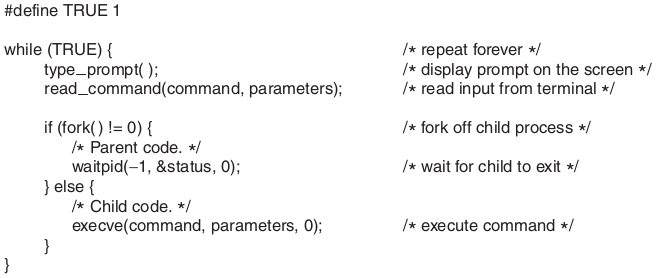
\includegraphics[width=0.75\textwidth]{FIG/1-19.png}
		\caption{一个精简的shell。贯穿全书,TRUE总是被定义为1。}\label{fig:simpleshell}
	\end{figure}

	在大多数的通常情况下,execve有三个参数:被执行文件的文件名,参数数组指针,环境数组指针,这些将会被很快地描述到。各种库过程,包括execl,execv,execle,execve,允许略掉参数或者以各种不同的方式指定。在本书中,我们在所有涉及的地方使用exec描述系统调用。让我们考虑一下向这样的命令:\texttt{cp file1 file2},是用来将file1复制到file2。在shell创建进程之后,该子进程定位和执行文件cp,并将源文件名和目标文件名传递给它。cp主程序(以及多数其他C程序的主程序)包括以下的声明:main(argc,argv,envp)。其中argc是命令行上的项目数的计数,包括程序名。对于上面的示例,argc是3。第二个参数argv是指向数组的指针。该数组的元素i是指向命令行上第i个字符串的指针。在我们的示例中,argv[0]将指向字符串“cp”,argv[1]将指向字符串“file1”,argv[2]将指向字符串“file2”。 
	%main函数的第三个参数,envp,是一个环境指针,是一个字符串数组,
	这些是程序可以获取环境变量的库过程,通常用于自定义用户希望如何执行某些任务(例如,要使用的默认打印机)。在图 \ref{fig:simpleshell} 中,没有环境变量被传递给子进程,因此exevc的第三个参数为0。
	如果exec显得过于复杂,不要绝望;它是最复杂的系统调用。其他的任何系统调用都更加简单。作为一个简单例子的系统调用,例如exit,完成执行时应该使用哪些进程。它有一个参数,退出状态(0到255),它通过\texttt{waitpid}系统调用中的\texttt{statloc}返回给父级。
	UNIX中的进程将内存分为三个段:文本段(程序代码),数据段(变量)和栈段。数据段向上增长,栈段向下增长,像图 \ref{fig:threesegments} 所示的那样。在它们之间是一段没有被使用的地址空间,堆栈会根据需要自动增长到间隙中,但数据段的扩展是通过使用系统调用brk显式完成的,brk指定数据段要结束的新地址。
	 
	\begin{figure}[ht]\small
		\centering
		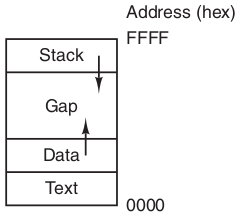
\includegraphics[width=0.75\textwidth]{FIG/1-20.png}
		\caption{一个进程有三个段:文本,数据和栈。}\label{fig:threesegments}
	\end{figure}
	
	数据段的扩展是显示通过一个系统调用brk实现的,它确定了数据段结束的新的地址。然而这个系统调用是没有被POSIX标准定义的,因为程序员被鼓励使用\texttt{malloc}库过程来动态分配内存,而\texttt{malloc}的底层实现则不是一个适合标准化的主题,因为几乎没有程序员直接使用它。我们甚至会注意到brk是不在系统调用之中的。
	
	\subsection{文件管理的系统调用}
	
	许多系统调用与文件系统相关。在本节中我们将看一下操作单个文件的系统调用。我们将在下一下涉及到目录或整个文件系统。为了读取和写一个文件,文件首先要先被打开。这个调用确定被打开的文件名,这个调用通过指定一个绝对的路径名和一个相对的工作目录名来指定要打开的文件名称,如代码O\_RDONLY,O\_WRONLY或者O\_RDWR意味着只读,只写和读写均可以。为了创建一个新的文件,会使用O\_CREAT参数。返回的文件描述符可以读或者写,接着,可以通过\texttt{close}系统调用关闭文件,它可以使文件描述符在后续的open中被再次使用。最经常被使用到的系统调用无疑是read和write。我们先看read系统调用,write系统调用拥有相同的参数。
	
	尽管大部分的程序是按照顺序访问文件的,但是一些应用程序需要能够随机访问文件的一部分。与每一个文件相关联的是一个指向文件当前位置的指针。当顺序地读或者写的时候,它经常会指向下一个被读/被写的字节。lseek系统调用改变了指针的位置,这样后续的read和write系统调用就可以在文件的任何位置停止。
	
	\texttt{lseek}有三个参数:第一个是文件描述符,第二个是一个文件位置,第三个是说明该文件位置是相对于文件起始位置,当前位置还是文件的末尾。lseek的返回值是改变指针后在文件中的绝对位置。
	
	对于每一个文件,UNIX跟踪文件模式(常规文件,特殊文件,目录等),大小,最后修改时间和一些其他的信息。程序可以通过调用stat系统调用看到这些信息。第一个参数指定了要被检查的文件,第二个参数指向一个指针,该指针指向存放这些信息的结构。对于一个打开的文件而言,fstat系统调用起到相同的作用。
	
	\subsection{目录管理的系统调用}
	
	在本节中,我们将讨论与目录和整个文件系统有关的系统调用,而不是上节中与某个文件有关的系统调用。mkdir和rmdir分别用于创建和删除目录,分别创建和移除空的目录。下一个调用是link,它的作用是允许一个文件以两个或多个名称出现,经常在不同的目录中。一个典型的应用是允许处在同一个编程小组的成员使用一个共同的文件,使得这个文件出现在他们每一个人的文件夹中,可能名字不同。共享一个文件并不等于给每一个成员一个私人副本,共享文件意味着任何成员所做的修改立即为其他成员所见--只有一个文件存在。而在复制了一个文件的多个副本之后,对其中一个副本所做的修改并不影响到其他的副本。
	
	为了看link是如何工作的,考虑一下图 \ref{fig:link} 所示的情形。这里有两个用户,ast和jim。每一个用户的目录下都有一些文件的。若ast现在执行一个包含系统调用的程序:link("/usr/jim/memo", "/usr/ast/note"),这个是将memo目录下的jim文件进入ast目录下的note文件。因此,/usr/jim/memo和/usr/ast/note指代的相同的文件。
	
	\begin{figure}[ht]\small
		\centering
		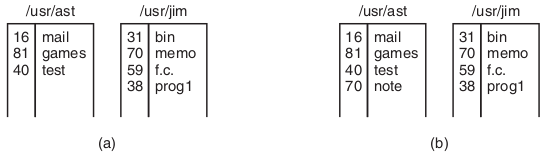
\includegraphics[width=0.75\textwidth]{FIG/1-21.png}
		\caption{a). 将/usr/jim/memo链接到ast目录之前的两个目录; b).链接后的两个目录}\label{fig:link}
	\end{figure}
	
	另外,用户目录是否保存在/usr、/user、/home或其他地方,这只是由本地系统管理员决定的。了解link是如何工作的可能会让它更清楚它的作用。UNIX中的每个文件都有一个唯一的编号,即标识它的i-节点号。这个i-节点号是i节点表的索引,每个文件一个,告诉谁拥有该文件,它的磁盘块在哪里等等。目录就是一个包含了对集合的文件。在第一个UNIX的版本中,每一个目录项是16字节,2字节的i节点号,14字节的文件名。现在,一个更复杂的结构用来支持更长的文件名。但是从概念上说,目录仍然是一个包含了若干文件的集合的文件。link所做的工作只是利用某个文件的i节点号,创建一个新的目录项。在图 \ref{fig:link}(b) 中,两个目录项拥有相同的i节点号,因为指向同一个文件。如果其中的任何一个稍后被删除了,如使用unlink系统调用,剩下的一个还在。如果两个都被移除了,UNIX看到尚且存在的文件没有目录项(i节点中的一个域记录着指向该文件的目录项),就会把该文件从磁盘中移去。
	就像我们之前提及的那样,\texttt{mount}允许将两个文件系统合并成一个文件系统。一个通常的情况是拥有根文件系统,包括经常使用命令的二进制(可执行)版本和其他一些经常使用的文件。在一个硬盘(子)分区上,用户文件在另一个(子)分区上。此外,然后用户可以插入一个包含要读取的文件的U盘。通过执行mount系统调用,USB文件系统可以被挂载到根文件系统上,像图  所示。
	一个典型的C语句完成mount操作的是:mount("/dev/sdb0", "/mnt", 0)。
	其中,第一个参数是USB设备的块特殊文件名,第二个参数是被挂载到目录树上的位置,第三个参数是告诉根文件系统被挂载的文件系统是读写的还是只读的。
	
	\begin{figure}[ht]\small
		\centering
		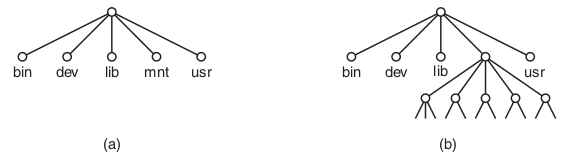
\includegraphics[width=0.75\textwidth]{FIG/1-22.png}
		\caption{a). 挂载前的目录树; b).挂载后的目录树}\label{fig:mount}
	\end{figure}

	在mount系统调用之后,一个在设备0上的文件可以使用从根目录或者工作目录的路径进行访问,而不用管文件在哪个设备上。事实上,还可以在这个树上挂载第二个,第三个,第四个设备。mount调用可以将可移动媒体集成到单个集成的文件层次结构,不必担心文件在哪个设备上。尽管这个例子讲述的是CD-ROM,但是可以用同样的方法挂载硬盘或硬盘的一部分,不管是外部的硬盘还是USB盘一样。当不再需要一个文件系统的时候,可以执行\texttt{umount}系统调用卸载文件系统。
	
	\subsection{各种系统调用}
	
	同样也存在着其他的系统调用。我们在这里只看他们其中的四个。\texttt{chdir}系统调用改变当前的工作目录,经过系统调用之后:
	chdir("/usr/ast/test"),将会打开一个xyz文件,/usr/ast/test/xyz,工作目录的概念消除了总是需要键入较长的路径名的需要。
	
	在UNIX中每一个文件都有一个用于保护的模式。这个模式包括针对所有者,组,其他拥有者的读-写-执行标志位。chmod系统调用可以改变文件的模式。例如,如果想改变某一个文件除了所有者之外为只读的,可以执行系统调用:chmod("file", 0644)。
	
	\texttt{kill}系统调用是用户和用户进程发送信号的方式。如果一个进程准备好了接收某一个信号,当它到达的时候,将会运行信号处理器。如果该进程没有准备好,那么信号的到来将会杀掉此进程(此调用名称的由来)。
	
	POSIX定义了一些处理时间的系统调用,如\texttt{time}系统调用,是以秒为单位返回当前时间,0对应着从1970年1月1日0时(从此时开始,没有结束)。在一台32位的计算机中,time的最大值是2$^{32}$-1秒(假设使用无符号整数)。这个值比136年稍大一些。因此在2106年,32位的UNIX系统就会变得发狂,与2000年对世界计算机造成严重破坏的Y2K问题是类似的。如果你现在有的是32位的UNIX系统,最好2106年之前换成64位的。
	
	\subsection{Windows Win32 API}
	
	到目前为止我们主要讨论UNIX,是时候讨论一下Windows了。Windows和UNIX的一个基本区别是他们的编程模型不同。UNIX系统包括各种处理事情的代码,使用系统调用执行特定的服务。与此相比,Windows通常是基于事件驱动的。主程序等待某一个事件的发生,然后调用一个程序去处理它。典型的事件有键盘被敲击,鼠标移动,鼠标按键按下或者插入了一个USB驱动。处理器将被调用来处理这些事件,更新屏幕和更新终端程序状态。所有的这些,都将会造成和UNIX不太一样的编程风格,但是由于本书的主题是讨论操作系统的功能和结构,我们将不会在关注这些编程模型的不同。
	
	当然,Windows也有系统调用。在UNIX中,系统调用和系统调用所使用的库过程几乎是一一对应的关系。换句话说,对于每一个系统调用,几乎都有一个触发它的库过程,像图 \ref{fig:read11steps} 所示中的那样。此外,POSIX有大约在100个过程调用。
	
	对于Windows,情况就大不相同了。首先,库调用和实际的系统调用是高度解偶的。微软定义了一组称为Win 32 API的过程调用供编程者使用获得操作系统的服务。这些接口支持所有的Windows 95以来的Windows操作系统版本。通过将API接口和实际的系统调用解偶,微软保持了在不改变现有程序的情况下随时改变系统调用的能力(甚至在每一个发行版本中进行改变)。
	
	是什么构成了Windows系统还是模糊不清的,因为最近版本的Windows有许多之前的版本所不包含的系统调用。在本节中,Win32意味着被所有版本的Windows支持的版本。Win32在Windows操作系统之间提供兼容性。
	
	Win 32 API的数量非常巨大,有上千个。此外,尽管它们中的许多触发系统调用,还是有大量的API完全是在用户态执行的。结果是在Windows无法分别哪个是系统调用(由内核执行),哪个是简单的用户空间库调用。事实上,在一个Windows版本中的系统调用可能在另一个版本中完全在用户态执行,反之亦然。当我们在本书中讨论Windows系统调用的时候,我们使用Win32过程,因为微软保障了随着时间的流逝,Win32过程将保持稳定。但是,值得记住的是并不是所有的它们都是系统调用(陷入到内核态)。
	
    Win 32 API有大量的系统调用,用来管理视窗,地理图标,文本,字体,滚动条,对话框,菜单以及GUI的其他特征。为了使得图形子系统运行在内核中(确实出现在某些版本的Windows中但不是所有的版本),需要系统调用,否则只有库调用。那么我们应该不应该在本书中讨论系统调用呢?由于它们和操作系统的功能并不相关,我们决定不讨论它们,尽管它们也是运行在内核中。对Win 32 API感兴趣的读者应该参考一些书籍中的相关内容(e.g., Hart, 1997; Rector and Newcomer, 1997; and Simon, 1997)。
    
   	尽管在这里介绍所有的Win32 API超出了问题的范围,所以我们只是将和UNIX系统调用功能大致相同的系统调用列出来在图 \ref{fig:win32APIs} 中。
   	
   	\begin{figure}[ht]\small
   		\centering
   		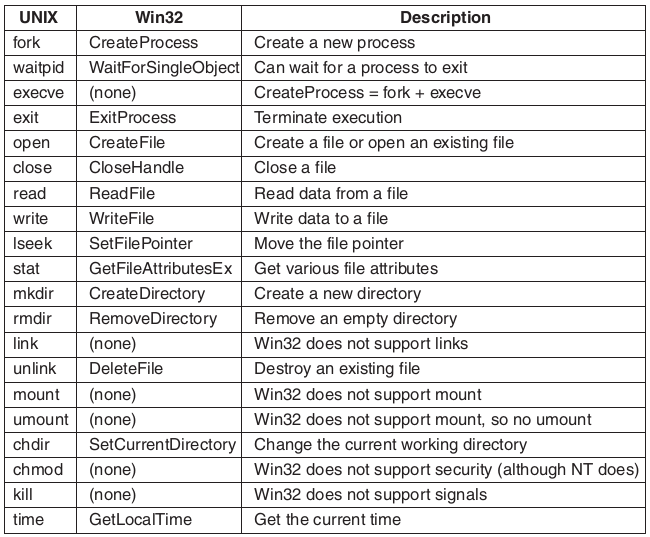
\includegraphics[width=0.75\textwidth]{FIG/1-23.png}
   		\caption{与UNIX大致对应的Win32 API} \label{fig:win32APIs}
   	\end{figure}
   
   现在让我们来简要看看图 \ref{fig:win32APIs} 中的内容。CreateProcess用于创建一个新的进程,它做的是UNIX中Fork加上execve的工作。它有许多的参数来指定新创建进程的性质。Windows不像UNIX那样具有进程层次结构,因为它不像UNIX一样具有父进程和子进程的概念。在一个进程创建后,创建者和被创建者是平等的。WaitForSingleObject被用来等待一个事件,可以等待许多可能的事件。如果有参数指定这个进程,调用者等待特定进程退出,通过调用ExitProcess完成。
   接下来操作文件的6个系统调用和UNIX的对应调用在功能上是类似的,尽管它们在参数和细节上有很多的不同。和UNIX中一样,文件可以被打开,关闭,读和写。SetFilePointer和GetFileAttributesEx调用用于设置文件位置和获取文件属性。
   Windows中有目录,它们使用创建目录CreateDirectory和删除目录RemoveDirectory API系统调用。也有对当前目录的标记,通过SetCurrentDirectory系统调用实现。使用GetLocalTime来获取当前的时间。
   
   Win32的接口不包括文件链接,挂载文件系统,安全,信号,所以对应与UNIX的这些调用就不存在了。当然,Win32也有大量的UNIX中没有的调用,特别是管理GUI的系统调用。Windows Vista有了一个精心设计的安全系统同时支持文件链接。Windows 7和8增加了更多的特征和系统调用。
   也许有必要对Win32做一下最后的说明,Win32并不是一个完全统一和一致的接口,最主要的原因是现有的32位Windows系统需要向后兼容16位的Windows 3.x系统。
   
   \section{操作系统结构}
   
   我们已经看到了操作系统从外面看是一种什么样的结构,现在是时候从里面看一下它的结构了。为了对各种可能的方式有所了解,我们将考察已经尝试过的6种不同的结构设计,这样并没有涵盖各种结构方式,但是至少给出了在实践中已经试验过的一些设计思想。我们将讨论的6种结构是:单体结构,分层结构,微内核,客户端-服务器模式,虚拟机和外核等。
   
   \subsection{单体系统}
   
   到目前为止最通常的组织形式,在单核系统方法中,整个操作系统在内核态以单一程序的形式运行。操作系统被写成是一堆过程调用的集合,互相链接起来称为一个大的可执行的二进制程序。当使用这个技术的时候,系统中的每一个过程可以自由地调用其他的过程,如果后者能够提供前者需要的y有用的计算的话。可以调用任何你想要的过程是非常高效的,但是有上千个可以互相调用,没有限制的过程也会导致一个系统笨拙且难以理解。
   同时,任何一个模块的崩溃都将会使整个操作系统陷入瘫痪。
   
   当使用这种方法来构建一个真正的操作系统目标程序的时候,首先编译所有的单个过程(或者是包含过程的文件),然后使用系统链接器将他们绑定成一个大的单个可执行文件。在信息隐藏方面,基本上没有-每一个过程都会其他的过程可见(相反,结构中有模块和包,大部分的信息都隐藏在包里面,而且只能通过正式设计的入口点实现模块的外部调用)。
   
   即使是在单体系统中,也是有一些结构存在的。操作系统所提供服务(系统调用)的参数被要求放在一个特定的位置(栈中)然后执行一个trap指令这个指令将机器从用户态切换到核心态,并且将控制权转交给操作系统,就像图 \ref{fig:read11steps} 中的第6步那样。
   操作系统接着就取出参数决定执行哪一个系统调用,接着它查询一个索引表将表中第k个槽位中存放着指向系统调用k过程的指针(图 \ref{fig:read11steps} 中的第7步)。
   
   对于这种类型的操作系统的结构,有着如下结构上的建议:
   1) 需要一个主程序来调用所要求的服务过程;
   2) 需要一套服务过程,用来执行系统调用;
   3) 需要一套实用过程,用来辅助服务过程。
   在这个模型中,每一个系统调用都有一个服务过程为其工作并执行它。要有一组实用程序来完成服务过程所需要用到的功能,如从用户程序中取出数据等。可以将过程分成一个三层的模型,如图 \ref{fig:monolithic} 所示。
   
   \begin{figure}[ht]\small
	   \centering
	   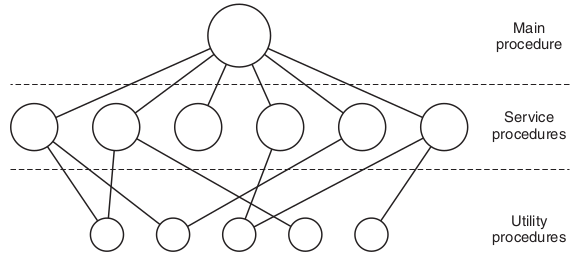
\includegraphics[width=0.75\textwidth]{FIG/1-24.png}
	   \caption{简单的单体系统结构模型} \label{fig:monolithic}
   \end{figure}
   	
   除了在计算机启动的时候加载核心操作系统之外,许多操作系统支持可加载的扩展模块,像I/O设备驱动和文件系统,这些组件是按需加载的。在UNIX中它们被称为共享库(shared library),在Windows中它们被称为动态链接库(Dynamic Link Library,DDL)。它们的文件扩展名为ddl,在\texttt{C:$\backslash$Windows$\backslash$system32}目录下有1000多个系统调用。
   
   \subsection{分层系统}
   
   把图 \ref{fig:monolithic} 中的结构进一步通用化,就形成了一个层次式结构的操作系统,它的上层软件都是基于下一层软件的基础之上构建的。E. W. Dijkstra (1968)和他的学生在荷兰的Eindhoven技术学院所开发的THE系统是第一个按照此结构构建的操作系统。THE系统是为一种荷兰的计算机Electrologica X8设计的一种简单的批处理系统,其内存只有32K个字,每个字有27位(那时二进制位是非常昂贵的)。
   
   如图 \ref{fig:layered} 所示,这个系统分为6层。第0层进行处理器分配,在中断发生或计时器过期时在进程之间切换。在第0层之上,系统由一些连续的进程组成,每一个进程都可以被编程而不用担心多个进程运行在一个处理器上的事实。也就是说,第0层提供了基本的CPU多道程序设计功能。
	
   \begin{figure}[ht]\small
		\centering
		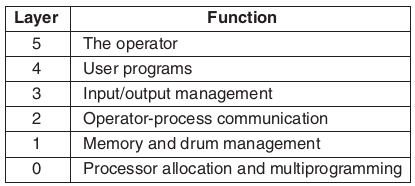
\includegraphics[width=0.75\textwidth]{FIG/1-25.png}
		\caption{THE操作系统的结构} \label{fig:layered}
   \end{figure}

	第一层是内存管理。它在主存中为进程分配内存,当内存用完时在一个512字节的磁鼓上保留进程的一部分页面。在第一层之上,不需要担心进程是在内存中还是在磁鼓上运行,第一层的软件保证一旦需要某一个页面,该页面必定已在内存中,并在页面不需要的时候将其移出。第2层处理进程和操作员控制台(即用户)之间的通信。第3层负责管理I/O设备,并对进出它们的信息流进行缓冲。第4层是用户程序层,他们不需要担心进程,内存,控制台或者I/O管理。系统操作员进程位于第5层中。在MULTICS中采用了更进一步的通用层次化概念,与分层不同的是,MULTICS被描述为一组同心圆,内部的圆比外部的圆拥有更高的优先权限(他们实际上是一样的)。当一个外环的过程调用内环的过程的时候,它必须执行一条等价于TRAP的指令,在执行该指令前,要进行严格的参数合法性检查。在MULTICS中,虽然整个操作系统是每个用户进程地址空间的一部分,但硬件使得能够指定单个过程(实际上是内存段)以防读、写或执行。尽管THE的分层方案只是一个设计上的辅助,因为在MULTICS中所有的部分都链接成一个可执行的程序,环机制在运行时非常常见并且由硬件强制执行。环形机制的好处是它可以轻易地扩展成用户子程序。例如,一个教授可以在第n环中设计给学生的考试程序并打分,而学生程序运行在第n+1环,这样的话他们就不可以改变他们的分数。
	
	\subsection{微内核}
	
	在分层的方法中,设计者有一个选择在哪里甚至内核态与用户态的边界。传统地说,所有的层次是运行在内核中的,但是它不是必须的。事实上,一个强有力的理由是尽可能少地使用内核模式,因为内核中的一个错误可以使得程序立即崩溃。相反的是,可以将用户进程设置为较小的权限,这样某个错误的后果也将不是致命的。不同的研究者已经研究了每1000行代码中bug的数量(e.g., Basilli and Perricone, 1984; and Ostrand and Weyuker, 2002)。Bug的密度取决于模块大小,模块的使用年限,对于商用工业系统而言,一个大约的数字是每1000行代码中有2-10个bug。
	这就意味着一个有着500万行代码的单体操作系统中,大约会有10000-50000个内核错误。当然,并不是所有的错误都是致命的。比如给出了不正确的故障错误信息等错误,实际上是很少发生的。不管怎么样,计算机是充满着大量的错误的,所以计算机的制造商设置了复位按钮(通常是在面板的前面)。而电视机,立体音箱和汽车的制造商却不这么做,尽管这些装置中也包含着大量的软件。
	微内核设计的一个基本想法是通过将操作系统分割成为小的,良好定义的模块来实现高可用性,只有其中的一个模块-微内核-运行在内核态,其余的模块由于功能相对弱一些,则作为普通用户程序运行。特别地,通过运行每一个设备驱动和文件系统作为一个独立的用户进程,如果一个bug出现,会导致这个组件失败,但是不会导致整个系统的崩溃。因此,音频驱动器中的一个bug将会导致声音断续或停止,但是不会使得电脑崩溃。相反,在单体系统中,所有的设备驱动都是在内核态中的,一个有bug的音频驱动程序很容易地引发对无效地址的引用,从而造成恼人的系统立即停机。
	许多微内核系统已经被实现和应用了数十年(Haertig et al., 1997; Heiser et al., 2006; Herder et al., 2006; Hildebrand, 1992; Kirsch et	al., 2005; Liedtke, 1993, 1995, 1996; Pike et al., 1992; and Zuberi et al., 1999)。除了基于Mach微内核的OS X之外,通常的桌面操作系统并不使用微内核。然而,它们在实时系统,工业系统,航空系统和军事应用中用地却非常广泛,这些领域都是关键任务,有很高的可靠性要求。知名的微内核有Integrity,K42,L4,PikeOS,QNX,Symbian,和
	MINIX 3。我们在这里简要地介绍一下MINIX 3,该操作系统把模块化的思想推向了极致,它将大部分的操作系统分解成许多独立的用户态进程。
	MINIX 3是一个POSIX兼容的,完全开源的操作系统,并且可以在www.minix3.org获得免费的开源源代码(Giuffrida et al., 2012; Giuffrida et al., 2013; Herder et al., 2006; Herder et al., 2009; and Hruby et al., 2013)。
	MINIX3微内核大约只有12000行C代码和1400行用于底层功能实现的汇编代码,如获取中断,切换进程等。C代码管理和调度进程,处理进程间通信(通过在进程间进行消息传递),提供大约40个内核调用,它们使得操作系统的其他部分可以完成其工作。这些调用完成诸如连接中断句柄,在地址空间中移动数据以及为新创建的进程安装新的内存镜像等功能。MINIX3的进程结构如图 \ref{fig:minix3} 所示,其内核调用句柄用\texttt{Sys}表示。时钟设备驱动也在内核中,因为这个驱动和调度器交互密切。所有的其他设备驱动都做为单独的用户进程进行。
	
    \begin{figure}[ht]\small
		\centering
		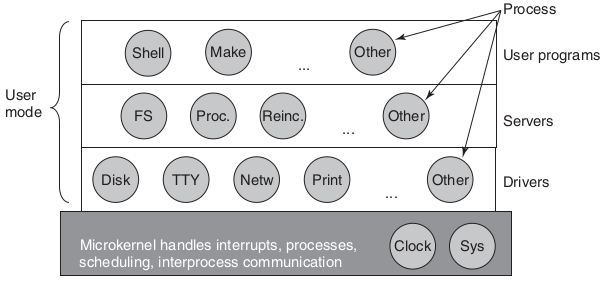
\includegraphics[width=0.75\textwidth]{FIG/1-26.png}
		\caption{MINIX3操作系统的结构} \label{fig:minix3}
	\end{figure}
	
	在内核的外部,系统的构造有三层进程,他们都在用户态运行。最底层包括设备驱动,因为它们运行在用户态,他们没有对I/O端口空间的物理地址,不能够直接执行I/O指令。相反地,为了编程一个I/O设备,驱动器构建一个结构,告诉向哪个I/O接口中设置什么值,并进行一个内核调用告诉内核去写。这种方法意味着内核可以检查驱动程序是否正在从它被授权使用的I/O中写入(或读取)。因此(与单片设计不同的是),一个有缺陷的音频驱动程序不会意外地写磁盘。在驱动层之上是另一个包含服务的用户模式层,它承担了操作系统大部分的工作。一个或多个文件服务器管理文件系统,进程管理器创建,销毁和管理进程。用户程序通过向服务器发送短消息请求POSIX系统调用来获得操作系统服务。例如,需要进行读取的进程向其中一个文件服务器发送一条消息,告诉它要读取什么。一个有趣的服务器是再生服务器(reincarnation server)。它的工作是检查其他的服务器和驱动是否在正确地工作。在这个过程中,如果发现一个有错误的,它将会被自动地被替换,而无须任何用户的参与。这种方式使得系统具有自修复能力,并且获得了较高的可靠性。系统有很多的方法来限制进程的权限。像前面提到的,驱动程序只能触及授权的I/O端口,对内核调用的访问也是按照单个进程控制的。这是考虑到进程具有向其他多个进程发送消息的能力。进程还可以授予其他进程有限的权限内核访问它们的地址空间。
	例如,一个文件系统可以给磁盘驱动器有限的许可,让内核在文件系统地址空间的固定位置进行对盘块的读入工作。总体来说,所有的这些限制都是为了让每一个驱动程序和服务器只拥有完成其工作的权限,这就大大限制了故障部件可能造成的危害。
	一个与小内核相关联的思想是内核中机制与策略相分离的原则。为了更清晰地明白这一点,让我们考虑一下进程调度。一个相对简单的调度算法是给每一个进程赋予一个数字优先权,内核运行拥有最高权限的进程。在这里,机制(在内核中)就是找到最高优先权的进程并运行之。而策略,给每一个进程分配优先级,则可以在用户态进行。在这种方式下,策略和机制可以分离,进而可以使得内核更小。
	
	\subsection{客户端-服务器模式}
	
	一个微内核思想的略微变体是将进程分为两类,一类是提供服务的进程,称为服务器,一类是使用这些服务的进程,称为客户端。这个模式就是所谓的服务器-客户端模式。通常最底层是一个微内核,但是不是必须的,其本质是存在服务器进程和客户端进程。客户端进程和服务器进程之间的通信主要通过消息传递。为了获取一个服务,一个客户端进程构建一个它想要什么的消息并把它发给合适的服务。服务接着进行具体的工作并将结果返回。如果客户端和服务器正好是运行在同一台机器上,可以进行一定的优化,但是概念上说,这里讨论的还是消息传递。
	这个思想一个显然的普遍模式是,客户端和服务器运行在不同的计算机上,他们通过局域网或者广域网连接,像图 \ref{fig:client-server} 所示的那样。
	
    \begin{figure}[ht]\small
		\centering
		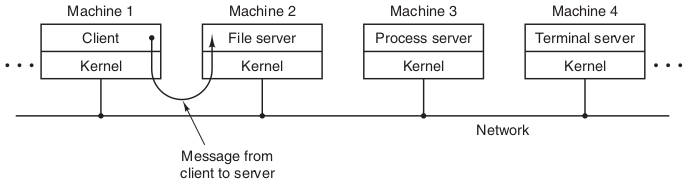
\includegraphics[width=0.75\textwidth]{FIG/1-27.png}
		\caption{一个位于网络上的客户端-服务器模式} \label{fig:client-server}
	\end{figure}

	因为客户端是通过发送消息和服务器进行通信的,所以客户端其实并不需要知道消息是否在它所在的本地机器进行处理或者是通过网络发送给一个远程的机器。对于客户端而言,这两种请求是一样的:都是发送请求并得到回应。所以,客户端-服务器模式是一种可以应用在单个机器或者一组网络机器的抽象。许多系统,包括用户家里的PC,都成为客户端,在别处运行的大型机器为服务器。事实上,许多Web就是以这个方式运行的。一台PC像一台服务器发送一个网页的请求,服务器返回网页请求。这是一个网络中客户端-服务器模式的典型应用方式。

	\subsection{虚拟机}
	
	OS/360系统最初是一个严格的批处理系统。许多360的用户希望能够在终端上交互工作,所以不同的组,包括IBM内部和外部的,决定为360写一个分时复用系统。后来推出了正式的IBM分时系统TSS/360,但是它非常庞大,运行缓慢,在花费了近5000万美元的研发费用之后还是被弃用了。但是在麻省剑桥的IBM科学研究中心的小组,开发了另一个完全不同的系统,该系统最终被IBM接受为产品。它的直接后代,称为z/VM,目前被IBM广泛地应用于大型机上,例如,zSeries在大型企业数据中心中被大量使用,例如,作为电子商务服务器,每秒处理数百或数千个事务,并使用大小达数百万GB的数据库。
	
	\textbf{VM370}
	
	这个系统,一开始叫做CP/CMS,后来重新命名为VM/370。它是源于一个机敏的观察,即分时系统应该提供这些功能:(1)多道程序 (2) 一个比裸设备带有更方便接口的扩展机器。VM/370的实质是分离这两个功能。系统的核心,被称为虚拟机监视器(VMM),运行在裸设备之上并且进行多道程序设计,向上层提供不是一个而是若干台虚拟机,像图 \ref{fig:vm370} 所示的一样。
	
    \begin{figure}[ht]\small
		\centering
		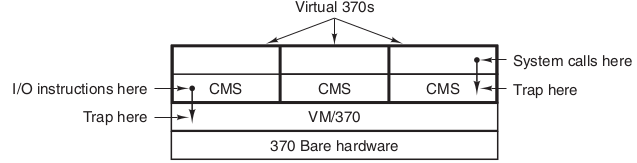
\includegraphics[width=0.75\textwidth]{FIG/1-28.png}
		\caption{配有CMS的VM370结构} \label{fig:vm370}
	\end{figure}

	然而,和其他操作系统不同的是,这些虚拟机并不是具有文件以及其他特征的扩展的机器,与之相反,它们是裸机硬件的完美复制品,包括内核态/用户态,I/O,中断以及一些其他硬件所具备的所有其他功能。因为每一个虚拟机和真实的硬件是类似的,每一个都可以运行直接在裸露机器上运行的任何操作系统。不同的虚拟机可以运行不同的操作系统,而且往往就是如此。在原始的IBM VM/370系统上,一些运行OS/360系统或者其他大型批处理和事务处理操作系统,其他运行单用户,交互式系统供分时用户使用,这个系统称为会话监控系统(Conversational Monitor System),后者在程序员中很流行。当一个CMS程序执行系统调用的时候,系统调用陷入到虚拟机自己的操作系统中,而不是VM/370系统上。好像它运行在一个真实的机器上而不是虚拟机上。CMS接着发出普通的硬件I/O指令读取它的虚拟磁盘或者它需要的任何其他东西来执行系统调用。这些I/O指令被VM/370陷入,然后,作为对实际硬件模拟的一部分,VM/370完成指令。通过完全分离多道程序功能和提供机器两者的完全分离,每个部分都变得更加地简单,更加地灵活和易于维护。虚拟机的现代化身z/VM通常是运行多个完整的操作系统而不是运行简化成像CMS那样的单用户系统。例如,zSeries有能力和IBM的操作系统一起,运行一个或多个Linux操作系统。
	
	\section{虚拟机的再次发现}
	
	IBM拥有虚拟机产品已经有40年了,一些其他的公司,包括Oracle,HP公司,在它们的高端服务器产品中增加了虚拟机的支持,而在PC上,虚拟机的思想直到最近以前一直被忽视了。但是在过去的一些年中,新的需求,新的软件,新的技术使得虚拟机又成为一个热点。首先是需求。许多公司将他们的邮件服务器,Web服务器,FTP服务器以及一些其他的服务器放在不同的计算机上,有时候使用不同的操作系统。他们把虚拟机看作是将这些服务放在同一台机器上而不用担心其中的一个服务崩溃影响到其他的服务。虚拟化在Web托管世界里也很流行。没有虚拟化,Web托管客户端只能在共享托管(这只是给他们一个在Web服务器上的登录账户,而对服务器的软件没有控制权)和直接托管(给它们自己的机器,这个方法非常地灵活,但是对于小型和中型的网站而言,成本效益比不高)之间进行选择。当Web托管公司提供租用的虚拟机时,一台物理机器就可以运行好多台虚拟机,而每一台虚拟机都可以看做是一个独立的机器。租用虚拟机的客户可以运行他们想要运行的任何操作系统和软件,但是只需要支付独占一台机器几分之一的费用(因为一台物理机器可以同时支持多台虚拟机)。虚拟化的另一个作用是给那些想在一台机器上运行一个或多个操作系统的终端用户使用,像Windows和Linux,因为他们最喜欢的程序包有的运行在这个操作系统上有的运行在那个操作系统上。这种情形就像图 \ref{fig:hypervisor} (a)所示的那样,在这里
	术语"虚拟机监视器"已经被重新命名为第一类虚拟机管理程序(type 1 hypervisor),这个名称现在更常用因为"Virtual  Machine Monitor"已经超出了人们可以承受的最大按键次数。但是请注意,许多作者可以互换使用这些术语。
	
    \begin{figure}[ht]\small
		\centering
		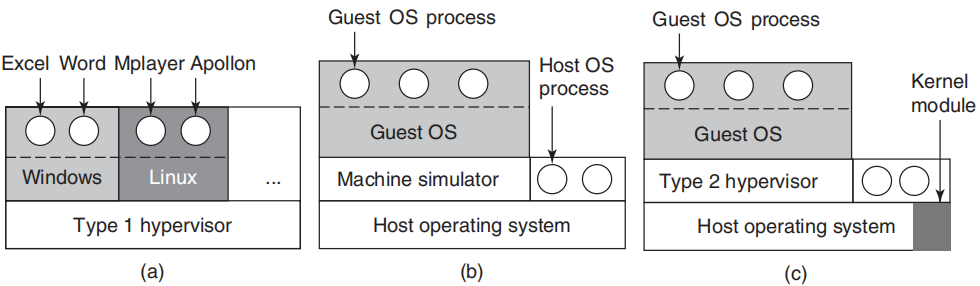
\includegraphics[width=0.75\textwidth]{FIG/1-29.png}
		\caption{a).第一类虚拟机管理程序 b).理论上的第二类虚拟机管理程序 c).实际上的第二类虚拟机管理程序} \label{fig:hypervisor}
	\end{figure}
	
	尽管没有人怀疑虚拟机的吸引力,但是问题是如何实现。为了能在一台计算机上运行虚拟机,它的CPU必须可以虚拟化。简而言之,问题就在这里。当一个运行在虚拟机上的操作系统执行一个优先权指令的时候,像修改PSW和执行I/O。必须将硬件陷阱设置到虚拟机监视器上,这样才能在软件中模拟指令。在一些CPU上(特别是Pentinum和它的后继者及克隆版中)试图在用户态执行特权指令时,会被忽略掉。这种属性使得在这个硬件上无法使用虚拟机,这也解释了PC世界对虚拟机不感兴趣的原因所在。但是也有一些Pentinum的解释器,比如Bochs,但是这种解释器会带来1-2个数量级上的性能损失,在一些要求高的工作场合失去了实际的应用价值。然而,这种情况在上世纪90年代末和本世纪初期因为一些学术研究工程的开展而改变,特别是斯坦福的Disco,剑桥大学的Xen,这些研究论文导致了一些商业产品的诞生(VMWare Work Station和Xen)和对虚拟机研究兴趣的重新滋生。除了VMWare和Xen,现在流行的虚拟机还有KVM(为Linux内核而建的),Virtual Box(由Oracle开发)和Hyper-V(由Microsoft开发)。
	这些早期的研究工程通过在线翻译代码块改善了类似Bochs之类的解释器的性能,并把它们保存在内部的Cache中,并在它们执行的时候重新使用它们。这在一定程度上改善了性能,也导致了我们称为机器模拟器的诞生,像图 \ref{fig:hypervisor}(b) 所示的那样。尽管这项被称为二进制翻译的技术对改善性能起到了一定的作用,其结果也足够优秀在学术会议上发表论文,但是这在十分重视性能的商业环境中还是远远不够的。
	下一个改善性能的步骤是加入一个添加分担重担的内核模块,像图 \ref{fig:hypervisor}(c) 所示的那样。在现实中,所有的商用的虚拟机,像VMWare Work Station,使用混合策略(当然也有许多其他的改进)。它们被称为类型2虚拟机,所以我们将在本书中沿用此称谓,甚至我们更倾向于称它类型1.7虚拟机来反映其并不完全是用户态程序的事实。在第7章中,我们将具体地描述VMWare Work Station是如何工作的,以及各部分的作用。
	实际上,类型1虚拟机和类型2虚拟机的真正区别是,类型2使用一个宿主操作系统以及它的文件系统来创建进程,存储文件等。而类型1虚拟机没有类似的底层支持,必须自己做这些功能。当类型2的虚拟机启动后,它读取客户操作系统所安装的CD-ROM(或者CD-ROM镜像文件),并将客户操作系统安装在一个虚拟磁盘上,它只是宿主操作系统的文件系统中一个巨大的文件。类型1虚拟机不能做这个是因为它没有宿主操作系统来存储文件
	。它们必须在一个原始的磁盘分区上自己做存储管理。当客户机操作系统被启动后,它做的事情和在真实的硬件上做的事情是一样的,典型的动作是启动一些后台进程进而启动GUI图形用户界面。对于用户,客户机操作系统表现地像它做裸金属设备上表现得一样,尽管实际是已经不是那么回事了。处理控制指令的另外一个方法是修改操作系统并移除它们,这个方法不是真正的虚拟化,而是半虚拟化。我们将在第7章中详细讨论虚拟化。
	
	\textbf{Java虚拟机}
	
	虚拟机使用的另外一个领域,但是又有所不同的是用于Java程序。当SUN公司发明了Java编程语言,它也发明了一个叫做Java虚拟机(Java Virtual Machine)的虚拟机(一种计算机体系结构)。Java编译器为JVM产生代码,这些代码接着被Java解释器的软件执行。这个方法的好处是JVM的代码可以通过网络传递到任何一台有Java解释器的机器上并在那里执行。如果编译器产生了SPARC或者X86的二进制程序,他们就不能随便被传播到哪里并运行了(当然,SUN公司也生产了一个产生SPARC二进制程序的编译器和一个分布式的SPARC解释器,但是JVM是一个简单很多的解释器架构)。使用JVM的另外一个好处是,如果解释器被正确地实现(当然这可不是一件小事),还要对JVM程序进行安全性检查,并在一个受保护的环境中执行,这样程序就不能盗取数据和做其他有害的操作了。
	
	\subsection{外核}
	
	和虚拟机克隆真实的机器不同,另一个策略是对其进行分区,换句话说,给每一个用户一个资源的子集。这个一个虚拟机可能会获得第0到1023个磁盘块,第二个虚拟机获取第1024到2047个磁盘块,以此类推。
	在底层,运行在内核态的,是一个被称为外核的应用程序。它的工作是为每一个虚拟机分配资源,并检查使用这些资源的企图,以确保没有别的虚拟机想要用其他虚拟机的资源。每一个用户级的虚拟机都可以运行它自己的操作系统,如VM/360和虚拟的奔腾8086,除非每一个已经被严格限制了只能使用为他分配的,他自己的资源。外核机制的另外一个好处是它节省了一层映射层。在其他的设计中,每一个虚拟机只考虑它自己的磁盘,数据块从0到一个最大值,所以虚拟机监控器必须维持一个重新映射磁盘地址的表格。而外核方案,就不需要这样。外核仅仅只需要记录哪一个虚拟机被分配到哪一个资源上了。这个方法仍然有可以分离多道程序(在外核中)和用户操作系统代码(在用户态)的好处,但是代价更小,外核所做仅仅是保证各个虚拟机不发生冲突。
	
	\section{依靠C语言的世界}
	
	操作系统通常是一个由很多编程者共同开发和很多模块的大型C(或者C++)程序。开发操作系统的环境和写Java小程序的环境是非常不同的。这个小节试图给有时候编写Java和Python程序的编程者介绍一下编写操作系统的环境。
	
	\subsection{C语言}

	这不是一个C语言的说明文档,而是介绍C语言和类似Python,特别是Java语言的一些关键不同之处。Java是基于C语言的,所以这两者有非常多的相似之处。为了方便起见,我们聚焦于Java。Java,Python和C都是命令式语言,有数据类型,变量和控制语句,例如,C语言中原始的数据类型是整型(包括长整型和短整型),字符型和浮点数。复合的数据结构可以使用数组,结构体和联合体。C语言中的控制语言和Java中的也非常类似,包括if,switch,for,while语句等。两种语言的函数和参数形式基本相同。C语言有的但是Java和Python没有的特征是显式指针。指针是指向变量(包括地址)或者数据结构的变量。考虑一下下面的语句:
	char c1, c2, * p;
	c1 = ’c’;
	p = \&c1;
	c2 = * p;
	以上语句声明了c1,c2两个字符变量,和一个指向字符变量的指针,第一个赋值语句将字符'c'的ASCII码存放在变量c1中,第二条语句将c1的地址赋值给指针变量p,第三条语句是将指向指针p的变量内容赋值给变量c2,所以这些语句执行以后,c2也包含了'c'的ASCII码。理论上,指针是类型化的,因此不应该将浮点数的地址分配给字符指针,但是实际的编译器接受这样的赋值,尽管有时候会发出警告。指针是一种非常强大的结构,但是如果使用不当,会是很多错误发生的根源。
	C语言没有的一些特征,包括内联字符串,线程,包,类,对象,类型安全和垃圾回收。最后一个是操作系统的"淋浴器塞子"。C语言中的存储都是编程人员静态或者显式分配和回收的,通常使用库函数\texttt{malloc}和\texttt{free}。正是由于后面的特性,由程序员完全操作内存-通过显式的指针,使得C语言对编写操作系统而言非常具有吸引力。操作系统在一定程度上是实时的系统,即使通用的操作系统也是这样。当中断发生的时候,操作系统通常只有若干微秒去处理发生的情况,否则就会有关键信息丢失,而且在任意时刻启动垃圾回收功能是不可接受的。
	
	\subsection{头文件}
	
	一个操作系统工程通常包括一定数量的目录,每一个都包含许多的c文件,这些文件存有系统某些部分的源代码,还有一些.h的头文件,包含被一个或多个源文件使用的声明和定义。头文件还可以包含一些简单的宏定义,像:\#define BUFFER\_SIZE 4096。
	允许编程者定义声明一些常量,所以当在代码中使用BUFFER\_SIZE变量的时候,它在编译的时候会被替换成数字4096。好的C语言编程习惯是对除了0,-1和1之外的变量进行命名,有时候甚至对0,-1和1进行命名。宏还可以带参数,例如: \#define max(a, b) (a > b ? a : b),允许编程者写i = max(j, k+1)和i = (j > k+1 ? j : k+1)来在i中存储j和k+1之间较大的一个。头文件还可以包含条件编译:
	\\\indent \#ifdef X86 
	\\\indent\indent  intel\_int\_ack(); 
	\\\indent \#endif
	\par 将会编译函数intel\_int\_ack()如果X86宏被定义的话,如果没有被定义的话则不编译。条件编译经常用来分离体系架构相关的代码,这样只有系统在X86体系结构上编译时才可以插入特定的代码,而其他的一些代码只有在SPARC架构下编译的时候才会被编译,等等。一个C文件,可以在头部使用\#include指令包含0个头文件和更多的头文件。也有很多和普通的c文件一样的头文件被存放在特定的目录下。
	
	\subsection{大型编程项目}
	
	为了构建操作系统,每一个c文件都被编译器编译成一个.o文件。后缀名为.o的目标文件包含着目标机器的二进制指令。它们稍后将会直接被CPU执行,在C语言的世界里,没有像Java和Python一样的字节码。C编译器的第一道是C预处理器。它读取每一个.c文件,每次遇到\#include指令的时候,它就将相应的头文件取来,并进行处理,扩展宏,处理条件编译(以及其他的事务),并且把结果传递给编译器的下一道,好像它们原先就包含这些头文件似的。因为操作系统非常地庞大(通常500万行代码是很正常的),当每次改变一个文件就需要对所有的东西进行重新编译是不可以接受的。另外一方面,改变一个被上千个其他文件包含的关键的头文件则确实需要重新编译这些文件。跟踪哪一个文件依赖于哪一个头文件在没有帮助的情况下是完全不可行的。幸运的是,计算机非常善于处理事物的分类。在UNIX系统中,有一个称为make的程序(还有一些其他的变种,如gmake,pmake等)来读取Makefile,告诉哪些文件依赖于哪些其他的文件。make要做的事情是检查为了构建操作系统二进制程序需要哪些目标文件,并且检查这些所依赖的文件(源代码和目标文件)是否在上一次被编译后被修改后,如果是,目标文件将需要被重新编译。当make程序需要决定重新编译哪一个c文件的时候,它就会触发c编译器来重新编译它们,进而将需要重新编译的文件降低到最少。在一些大型的工程中,创建makefile是一件非常容易出错的事情,但是现在已经有工具可以自动地做这件事了。当所有的.o文件都准备好了以后,它们被传递到一个叫做连接器的程序,来将它们组合成一个单个的可执行二进制文件。此时还包括调用的任何库函数,解析函数间引用,并根据需要重新定位主机地址。当连接器结束的时候,结果是一个可执行的程序,在UNIX系统中通常称为a.out程序。图 \ref{fig:compile} 给出了一个程序进程的不同组成部分,包括3个C程序和2个头文件。尽管我们在这里是讨论操作系统的开发,这些也都可以应用于任何一个大型的程序。
		
	\begin{figure}[ht]\small
		\centering
		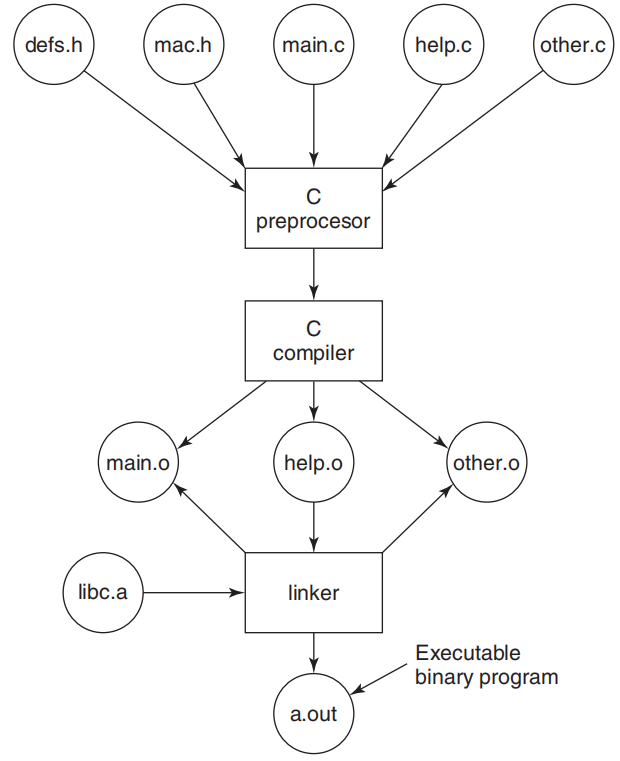
\includegraphics[width=0.75\textwidth]{FIG/1-30.png}
		\caption{编译一个C程序和头文件使得其可以运行的过程} \label{fig:compile}
	\end{figure}
	
	\subsection{运行时模型}
	
	当操作系统的二进制文件被链接的时候,计算机可以重启而且新的操作系统可以启动了。一旦运行,它可以动态地加载没有被静态地加载进来的操作系统部分,像设备驱动和文件系统。在运行时操作系统可以包括多个片段,像代码段,数据段和栈。代码段通常是不可改变的,在执行中不被改变。数据段从一定的大小开始,并用一些值进行初始化,但是它可以根据需要进行改变。栈一开始是空的,但是随着函数的调用和返回,栈开始增长和收缩。通常代码段被放置在接近内存的底部,数据段紧跟着在其之上,并且可以向上增长。栈段在高的虚拟地址,并且可以向下增长,但是不同的系统工作起来也不相同。在所有的情况下,操作系统的代码都是被硬件直接执行的,没有解释器和实时编译,这一点和Java很不相同。
	
	\section{操作系统的研究}
	
	计算机科学是一个高速发展的领域,很难预言它将会朝什么方向发展。在大学和工业界研究性质的实验室里的研究者们不断地想出新的想法,这些想法有一些变得不知所踪,而有一些则成为未来产品的基石,并且对工业界和用户产生了重要的影响。事后告诉哪些会怎样哪些会怎样总是比实时地告诉更加容易一些。而且分离小麦和麸糠是特别困难的因为它通常要花费20-30年才能将一个想法变为现实并且产生影响。例如,当美国总统埃森豪威尔在1958年设立国防部高级研究计划署的时候,他试图通过五角大楼的国防预算来试图阻止陆军对海军和空军的削弱,他不是试图发明互联网。但是APRA做的其中一件事情是资助一些大学研究研究在当时看来很荒诞的概念-包交换,这导致了第一个实验性包交换网络的诞生-ARPANET。它在1969年启用了。不久,APRA资助的其他网络和ARPANET也连接到了一起,于是因特网诞生了。于是因特网被学术研究者很高兴地用来收发邮件长达20年之久。在1990年代早期,蒂姆·伯纳斯·李在日内瓦的CERN的研究中心实验室发明了万维网,马克·安德森在伊利诺伊大学为其写了一个图形化的浏览器。突然之间,互联网上充满了年轻人的聊天,埃森豪威尔总统可能在他的坟墓里翻身了。操作系统的研究同样会导致实际的系统发生很大的变化。正如我们之前提到的那样,第一代的商用计算机系统都是批处理系统,直到M.I.T在1960年代发明了通用的分时系统。计算机在道格·恩格尔巴特发明鼠标之前都是基于文本的,在1960年代末期,斯坦福的研究机构发明了图形用户界面。在本节以及本书中可比较的其他章节中,我们将简要地回顾一下过去的5到10年之间操作系统领域的一些研究,这是为了让读者了解可能会发生什么。这个介绍当然不是综合性的,主要是基于在操作系统领域的顶级研究会议上发表的论文,因为这些论文能够发表肯定是经历了非常严谨的同行评审。要注意到在计算机领域-和其他的研究领域有所不同的是-大部分的好的研究成果是发表在会议上的,而不是期刊上的。大部分在研究章节被引用的论文都是发表在ACM,IEEE和USENIX上的,并且通过网络向它的用户(包括学生用户)开放。要获得这些组织机构和它们的图书馆更多的信息,可以通过以下网站:	
	\\\indent ACM http://www.acm.org

	IEEE Computer Society http://www.computer.org

	USENIX http://www.usenix.org
	事实上,所有的操作系统研究者们意识到当前的操作系统是庞大的,复杂的,不可靠的,不安全的,充满了错误,并且某一个操作系统比其他操作系统有着更多的错误(在这里略去名字以免承担责任)。结果,就出现了大量的研究工作来探讨如果构建一个更好的操作系统。近年来的研究工作有以下一些:关于错误和调试(Renzelmann et al., 2012; Zhou et
al., 2012),故障恢复(Correia et al., 2012; Ma et al., 2013; Ongaro et al.,2011; Yeh Cheng, 2012),电源管理(Pathak et al., 2012; Petrucci Loques, 2012; Shen et al., 2013),文件和存储系统(Elnably, Wang, 2012; Nightingale et al., 2012; Zhang et al., 2013a),高性能I/O(De Bruijn et al., 2011; Li et al., 2013a; Rizzo, 2012),超线程和多线程(Liu et al., 2011),动态更新(Giuffrida et al., 2013),GPU管理(Rossbach et al., 2011),内存管理(Jantz et al., 2013;
Jeong et al., 2013),多核操作系统(Baumann et al., 2009; Kapritsos, 2012; Lachaize et al., 2012; Wentzlaff et al., 2012),操作系统正确性(Elphinstone et al., 2007; Yang et al., 2006; Klein et al., 2009),操作系统可靠性(Hruby et al., 2012; Ryzhyk et al., 2009, 2011 Zheng et al., 2012),隐私与安全(Dunn et al., 2012; Giuffrida et al., 2012; Li et al.,
2013b; Lorch et al., 2013; Ortolani Crispo, 2012; Slowinska et al., 2012; Ur et al., 2012),用户和性能监控(Harter et. al, 2012; Ravindranath et al., 2012)和虚拟化(Agesen et al., 2012; Ben-Yehuda et al.,
2010; Colp et al., 2011; Dai et al., 2013; Tarasov et al., 2013; Williams et al.,2012)以及一些其他的许多主题。
	
	\section{本书剩余部分的结构}
	
	我们已经介绍了操作系统并且对操作系统形成了一个总体的概览。现在是时候开始深入到细节了。像已经提到的那样,从编程者的角度看,操作系统的主要目的是提供一些关键的抽象,其中最重要的是进程和线程,地址空间和文件。接下来的三章会集中讨论这些关键部分。
	
	第二章是关于进程和线程,讨论它们的属性以及它们之间是如何通信的,也给出了几个进程间通信是如何工作和如何避免陷阱的详细例子。
	第三章我们将详细学习地址空间和它的附属物:内存管理。将会讨论到虚拟内存这个重要的主题,以及一些紧密相关的概念,分页和分段等。
	第四章我们将讨论对所有都很重要的主题:文件系统。在相当的程度上,大部分情况下用户看到的是文件系统。我们将同时关注文件系统的接口和文件系统的实现。
	第五章是输入/输出系统。设备独立性和设备依赖性的概念将会被关注。一些重要的设备,包括磁盘,键盘,显示器等,将会被作为例子使用到。
	第六章是关于死锁。我们将在本章简要地展示什么是死锁,还有一些其他的更多内容,比如如何避免和预防死锁等。
	到了这里,我们将完成一个单CPU操作系统基本原则的学习。但是还有更多的内容需要讨论,特别是一些高级的主题。在第7章中,我们将讨论虚拟化。我们将同时讨论虚拟化的原则以及一些现有的虚拟化解决方案的例子。因为虚拟化在云计算中使用地很多,我们还将关注现有的云。另外一个高级主题是多处理器系统,包括多核,并行计算机和分布式系统。这些主题将在第8章中覆盖到。
	操作系统中一个非常重要的主题是安全,将在第9章中讨论。在该章将被讨论到的主题是:威胁(病毒和蠕虫),保护机制和安全模型。
	接下来我们将学习一些实际的操作系统按列,包括UNIX,Linux,Android(第10章)和Windows 8(第11章)。我们将在第12章介绍一些操作系统设计方面的智慧与思想。
	
	\section{公制单位}
	
	为了避免任何的混乱,值得我们在本书中显式地声明,为了计算机科学的通用性,使用公制单位代替传统的英制单位(the furlong-stone-fortnight system)使用。图 \ref{fig:metric-prefixes} 给出了主要公制前缀。前缀主要是缩写成它的首字母。凡是单位大于1的首字母都大写。这样,1TB的数据库占据$10^{2}$字节的存储,100 psec(100 ps)时钟每$10^{-10}$秒滴答一次。因为\texttt{milli}和\texttt{micro}都是字母'm'开头,所以必须要对这两者作出区分。通常用'm'表示\texttt{milli},用 \textmu(希腊字母)表示\texttt{micro}。
		
	\begin{figure}[ht]\small
		\centering
		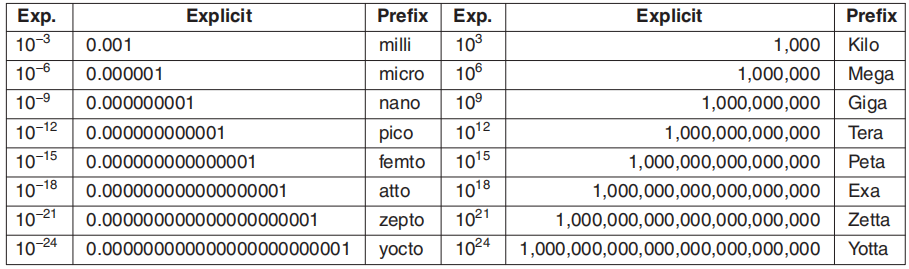
\includegraphics[width=0.85\textwidth]{FIG/1-31.png}
		\caption{主要的公制前缀}\label{fig:metric-prefixes}
	\end{figure}

	同时值得指出的是,在通常的工业实践中,测量存储容量大小的单位略微有所不同。如Kilo表示的$2^{10}$(1024)而不是1000,因为存储容量总是2的幂次方。因此1KB内存包含1024个字节,而不是1000个字节。相似地,1MB内存包含$2^{20}$(1,048,576)字节,1GB内存包含$2^{30}$(1,073,741,824)字节。但是,一条1-Kbps的通信线每秒传输1000比特,一个10-Mbps的局域网以每秒10,000,000位的速度运行,因为速度不是2的整数次幂。不幸的是,许多人会把这两个系统弄混淆,特别是磁盘的大小。为了避免混淆,我们在本书中使用KB,MB,GB表示$2^{10}$,$2^{20}$,$2^{30}$字节,而使用Kbps,Mbps和Gbps分别表示$10^{3}$,$10^{6}$和$10^{9}$bits每秒。
	
	\section{总结}
	
	操作系统可以从两个视角进行审视:资源管理者和扩展的机器。从资源管理者的角度,操作系统的工作是将系统的不同部分有效地管理起来。在扩展机器视角,操作系统的工作是提供用户比真实机器更加方便的抽象。这些包括进程,地址空间和文件。操作系统有很长的历史,从它们开始取代操作子开始,到现代的多道程序系统。亮点包括早期的批处理系统,多道程序系统和个人计算机系统。
	因为操作系统和硬件有很强的关联性,具备一些计算机硬件的知识将会有助于帮助理解它们。计算机是由处理器,内存和I/O设备组成的。这些部件通过总线连接。操作系统的基本概念就是基于进程,内存管理,文件系统,I/O管理和安全构成的。每一个部分都会在接下来的章节中依次讨论到。
	操作系统的核心是它可以处理的系统调用,这些将告诉操作系统真正如何使用。对于UNIX,我们看了四组系统调用,第一组系统调用是关于进程的创建和终止,第二组的是关于读写文件,第三组是关于目录管理,第四组则包括一些其他的系统调用。操作系统可以用多种方式进行组织,最常见的是单体系统,分层系统,微内核,客户机-服务器,虚拟机和外核。
	
	
	
	
	
	
	
	
	
	
	
	
	
	
	
	
	
	
	
	
	
	
	
	
	
	
	
	
	
	
	

	
	
	
	
	
	
	
	
	
	
	
	
	
	
	
	
	
	
	
	
	

%\setlength{\fboxrule}{0pt}\setlength{\fboxsep}{0cm}
%\noindent\shadowbox{
%\begin{tcolorbox}[arc=0mm,colback=lightblue,colframe=darkblue,title=学习目标与要求]
%\kai\textcolor{darkblue}{1.~~了解科学计算的一般过程.}\\
%\kai\textcolor{darkblue}{2.~~了解数值计算方法的研究内容和特点.}\\
%\kai\textcolor{darkblue}{3.~~理解数值计算误差的有关概念.}\\
%\kai\textcolor{darkblue}{4.~~掌握数值计算误差的控制方法.}
%\end{tcolorbox}}
%\setlength{\fboxrule}{1pt}\setlength{\fboxsep}{4pt}
%
%
%\section{Colored boxes}
%
%\begin{tcolorbox}[colback=red!5,colframe=red!75!black]
%  My box.
%\end{tcolorbox}
%
%\begin{tcolorbox}[colback=blue!5,colframe=blue!75!black,title=My title]
%  My box with my title.
%\end{tcolorbox}
%
%\begin{tcolorbox}[colback=green!5,colframe=green!75!black]
%  Upper part of my box.
%  \tcblower
%  Lower part of my box.
%\end{tcolorbox}
%
%\begin{tcolorbox}[colback=yellow!5,colframe=yellow!75!black,title=My title]
%  I can do this also with a title.
%  \tcblower
%  Lower part of my box.
%\end{tcolorbox}
%
%\begin{tcolorbox}[colback=yellow!10,colframe=red!75!black,lowerbox=invisible,
%  savelowerto=\jobname_ex.tex]
%  Now, we play hide and seek. Where is the lower part?
%  \tcblower
%  I'm invisible until you find me.
%\end{tcolorbox}
%
%\begin{tcolorbox}[colback=yellow!10,colframe=red!75!black,title=Here I am]
%  \input{\jobname_ex.tex}
%\end{tcolorbox}
%
%
%\begin{tcolorbox}[colback=blue!50,colframe=blue!25!black,coltext=yellow,
%    fontupper=\Large\bfseries,arc=6mm,boxrule=2mm,boxsep=5mm]
%  ofFunny settings.
%\end{tcolorbox}
%
%\subsection{\LaTeX-Table}
%
%\begin{table}[h]\begin{center}\color{darkblue}\caption{计算结果}\color{black}\label{tab1-2}
%{\footnotesize
%\begin{tabular}{r|r||r|r||r|r||r|r}\arrayrulecolor{darkblue}\hline\rowcolor{lightblue}
%  $n$&$I_n$&$n$&$I_n$&$n$&$I_n$&$n$&$I_n$\\\hline
%  19&0.008\ 3&14&0.011\ 2&9&0.016\ 9&4&0.034\ 3\\
%  18&0.008\ 9&13&0.012\ 0&8&0.018\ 8&3&0.043\ 1\\
%  17&0.009\ 3&12&0.013\ 0&7&0.021\ 2&2&0.058\ 0\\
%  16&0.009\ 9&11&0.014\ 1&6&0.024\ 3&1&0.088\ 4\\
%  15&0.010\ 5&10&0.015\ 4&5&0.028\ 5&0&0.182\ 3\\\hline
% \end{tabular}}\end{center}\end{table}
%
%
%\section{\LaTeX-Examples}
%
%\begin{tcblisting}{colback=red!5,colframe=red!75!black}
%This is a \LaTeX\ example:
%$\displaystyle\sum\limits_{i=1}^n i = \frac{n(n+1)}{2}$.
%\end{tcblisting}
%
%
%\section{Theorems}
%
%\begin{defi}{Summation of Numbers}{defi1.1}
%  For all natural number $n$ it holds:\\[2mm]
%  $\displaystyle\sum\limits_{i=1}^n i = \frac{n(n+1)}{2}$.
%\end{defi}
%
%\begin{theo}{Summation of Numbers}{theo1.1}
%  For all natural number $n$ it holds:\\[2mm]
%  $\displaystyle\sum\limits_{i=1}^n i = \frac{n(n+1)}{2}$.
%\end{theo}
%
%\begin{coro}{Summation of Numbers}{coro1.1}
%  For all natural number $n$ it holds:\\[2mm]
%  $\displaystyle\sum\limits_{i=1}^n i = \frac{n(n+1)}{2}$.
%\end{coro}
%We have given Theorem \ref{Theorem:theo1.1} on page \pageref{Theorem:theo1.1}.
%
%
%
%\begin{table}[h]\begin{center}\color{darkblue}\caption{计算结果}\color{black}\label{tab1-1}
%{\footnotesize
%\begin{tabular}{r|r||r|r||r|r||r|r}\arrayrulecolor{darkblue}\hline\rowcolor{lightblue}
%  $n$&$I_n$&$n$&$I_n$&$n$&$I_n$&$n$&$I_n$\\\hline
%  1&0.088\ 4&6&0.034\ 4&11&-31.392\ 5&16&9.814\ 5e+4\\
%  2&0.581\ 0&7&-0.029\ 0&12&157.045\ 7&17&-4.907\ 3e+5\\
%  3&0.043\ 1&8&0.270\ 1&13&-785.151\ 6&18&2.453\ 6e+6\\
%  4&0.347\ 0&9&-1.239\ 3&14&3.925\ 8e+3&19&-1.226\ 8e+7\\
%  5&0.026\ 5&10&0.296\ 7&15&-1.962\ 9e+4&20&6.134\ 1e+7\\\hline
%\end{tabular}}\end{center}\end{table}
%
%\section{graphicx}
%
%\begin{figure}[h]
%\begin{minipage}[t]{0.5\linewidth}
%\centering
%%\includegraphics[totalheight=1.2in]{fig/tu2-2}
%\caption{不动点迭代法收敛} \label{fig:tu2-2}
%\end{minipage}
%\begin{minipage}[t]{0.5\linewidth}
%\centering
%%\includegraphics[totalheight=1.3in]{fig/tu2-3}
%\caption{不动点迭代法发散} \label{fig:tu2-3}
%\end{minipage}
%\end{figure}
%
%
%
%\vspace{0.5cm}
%\addcontentsline{toc}{section}{\protect\numberline{}{习题一}}
%\markboth{习题一}{习题一} \centerline{\textcolor{darkblue}{\hei\zihao{4}
% 习题一}}\vspace{0.5cm}
%
%
